% _____________________________________________________________________________
%
%
%	     DOCUMENT HEADER
%
% _____________________________________________________________________________
%

\documentclass[english, ing, kiv, he, iso690numb, pdf]{fasthesis}
\title{ARMv6 Processor Emulator for Raspberry Pi Environment Emulation}
\author{Jakub}{Šilhavý}{Bc.}{}
\supervisor{Ing. Martin Úbl}
\assignment{zadani.pdf}
\signdate{14}{05}{2024}{V Plzni}% << the longest local name in the Czech Rep.

\usepackage{biblatex}
\usepackage{subcaption}
\usepackage{afterpage}
\usepackage{dirtytalk}

\addbibresource{DP_silhavyj_A21N0072P.bib}% << the file with the bibliographical database to be used throughout the text
% _____________________________________________________________________________
%
%
%	     DOCUMENT FRONTMATTER TEXTS
%
% _____________________________________________________________________________
%
\abstract{
	This paper examines the potential of emulating Raspberry Pi Zero, a selected example of one of the most widely adopted architectures for embedded systems — the ARM architecture. The initial chapters delve into a general introduction to the ARM architecture, highlighting its profound significance evidenced by billions of electronic devices that leverage it. Transitioning to the second part, the thesis addresses the benefits of utilizing an ARM emulator, delineating overall requirements, and reviewing existing methodologies.
	
	The second part centers on the development of a custom Raspberry Pi Zero emulator whose functionality is systematically tested using a set of examples pertinent to operating system development. The thesis concludes with an objective evaluation of the emulator's performance, identifying its key benefits, and suggesting areas for further enhancements.
}
% *** Czech abstract ***
{
	Diplomová práce se zabývá zkoumáním potenciálu emulace Raspberry Pi Zero, který reprezentuje jednu z nejrozšířenějších architektur pro vestavěné systémy - \break architekturu ARM. Úvodní kapitoly přinášejí obecné seznámení s ARM architekturou, jejíž významnost je demonstrována více než miliardou elektronických zařízení, které ji využívají. Dále se práce zaměřuje na výhody využívání ARM emulátoru, stanovení celkových požadavků a analýzu existujících možností řešení.
	
	Druhá část textu se soustředí na vývoj samotného Raspberry Pi Zero emulátoru, jehož funkčnost je systematicky testována pomocí sady příkladů vztahujících se k vývoji operačních systémů. Práce je zakončena objektivním hodnocením výkonu emulátoru, identifikací jeho klíčových výhod a navrhováním oblastí pro další \break vylepšení.
}
\keywords{ARM, Processor, Emulator, Raspberry Pi Zero}
% _____________________________________________________________________________
%
%
%	     DOCUMENT TEXT BEGINNING
%
% _____________________________________________________________________________
%

\newcommand\mainmatterWithoutReset
{
	\edef\temppagenumber{\arabic{page}}%
	\mainmatter
	\setcounter{page}{\the\numexpr\temppagenumber+2\relax}%
}


\newcommand\blankpage{%
	\null
	\thispagestyle{empty}%
	\addtocounter{page}{-1}%
	\newpage}


\begin{document}
	\frontpages[tm] % or notm if the `trademark' declaration is not needed
	
	\setcounter{tocdepth}{3}
	\tableofcontents
	
	% 
	% -x---- ADDITIONAL COLOUR DEFINITIONS ----------------------------------------
	%
	\makeatletter%
	\ifx\FASThesis@style\c@fullcolor%
	\definecolor{fascolor}{cmyk}{0.06, 0.27, 1.0, 0.12}%
	\definecolor{fascolordk}{cmyk}{0.05, 0.28, 1.0, 0.24}%
	\else%
	\definecolor{fascolor}{cmyk}{0, 0, 0, 0.6}%
	\definecolor{fascolordk}{cmyk}{0, 0, 0, 0.75}%
	\fi%
	\makeatother%
	\lstdefinestyle{plainsrc}{
		backgroundcolor=\color{fascolor!10},
		basicstyle=\ttzfamily\footnotesize,
		numberstyle=\tiny\color{fascolordk},
		numbers=left,
		numbersep=5pt,
		keepspaces=true,
		tabsize=2,
		extendedchars=true,
		literate={á}{{\'a}}1 {č}{{\v{c}}}1 {ď}{{\v{d}}}1 {é}{{\'e}}1 {ě}{{\v{e}}}1 {è}{{\`{e}}}1 {í}{{\'{\i}}}1 {ľ}{{\v{l}}}1 {ň}{{\v{n}}}1 {ó}{{\'o}}1 {ŕ}{{\'r}}1 {ř}{{\v{r}}}1 {š}{{\v{s}}}1 {ť}{{\v{t}}}1 {ú}{{\'u}}1 {ů}{{\r{u}}}1 {ý}{{\'y}}1 {ž}{{\v{z}}}1
		{Á}{{\'A}}1 {Č}{{\v{C}}}1 {Ď}{{\v{D}}}1 {É}{{\'E}}1 {Ě}{{\v{E}}}1 {È}{{\`{E}}}1 {Í}{{\'I}}1 {Ľ}{{\v{L}}}1 {Ň}{{\v{N}}}1 {Ó}{{\'O}}1 {Ŕ}{{\'R}}1 {Ř}{{\v{R}}}1 {Š}{{\v{Š}}}1 {Ť}{{\v{T}}}1 {Ú}{{\'U}}1 {Ů}{{\r{U}}}1 {Ý}{{\'Y}}1 {Ž}{{\v{Z}}}1
	}
	
	\setcounter{biburllcpenalty}{100}
	\setcounter{biburlucpenalty}{100}
	\setcounter{biburlnumpenalty}{100}
	
	\biburlnumskip=0mu plus 1mu\relax
	\biburlucskip=0mu plus 1mu\relax
	\biburllcskip=0mu plus 1mu\relax
	
	\chapter{Introduction}
	
	Over the past several years, ARM \footnote{The term ARM is commonly recognized as an acronym, initially representing \textit{Acorn RISC Machine} before being redefined as \textit{Advanced RISC Machine}.}, as a computer architecture, has garnered popularity across a wide array of applications. Its usage spans from low-power solutions and affordable microcontrollers to real-time applications and safety-critical systems that include medical devices, automotive technology, and aviation. Furthermore, ARM is extensively utilized in personal computers and the cell phone industry. Presently, it is estimated that ARM powers over 99\% of the world's smartphones \cite{ARM-history}. Covering such a diverse range of applications, ARM has tailored its processor cores into various groups known as families. Notable among these is ARMv6, employed in devices like Raspberry Pi Zero. This version introduced innovative technologies such as \textit{TrustZone}, \textit{Jazelle}, and \textit{Single Instruction/Multiple Data} instructions to the Classic line of ARM processor cores.
	
	Emulating such a widely adopted architecture can assist in illustrating concepts of computer organization and operating system principles. In addition to educational purposes, the use of an ARM emulator can prove beneficial in the software development process, particularly when immediate access to a development board may not be feasible. Furthermore, it provides a safety net by enabling developers to experiment with potentially risky code without concerns about damaging real hardware. As a software tool, it could also be integrated into continuous-integration automated testing to identify potential bugs before moving on to testing on actual hardware, which may not be readily available.
	
	This thesis delves into the fundamental principals of the ARM architecture, exploring and evaluating existing emulation solutions tailored for an embedded environment. The primary goal is to design, implement, and rigorously test a comprehensive and extensible Raspberry Pi Zero emulator capable of emulating KIV-RTOS \cite{KIV-RTOS} — a real-time operating system developed for educational purposes at the University of West Bohemia.
	
	\chapter{Computer Architectures}
	
	A computer architecture can be generally considered a low-level principal design of a computer system that defines the interaction of its components that work alongside to accomplish a given task. While there are a number of different computer architectures, some of the most widely recognized may include Intel, MIPS, ARM, or the increasingly popular RISC-V architecture \cite{harvard-architecture-1}.
	
	The internal workings of a computer architecture can be explained through the concept known as \textit{Instruction Set Architecture}, often abbreviated as \texttt{ISA}, which provides a comprehensive understanding of computer's operation capabilities. It also provides insights into how the user can interact with the central processing unit, the \texttt{CPU}, based on the specific types of instructions it supports. 
	
	\section{Classification of Computer Architectures} \label{Classification of Computer Architectures}
	
	\textbf{Computer architectures can be categorized by various aspects}, such as how they handle data, the addressing modes they support, how they organize memory, what register set they feature \footnote{Although registers are the fastest type of memory, from an operating system perspective, featuring an extensive number of registers can also pose a disadvantage, as it increases the time required to perform a context switch, which might be critical for real-time applications.}, or the number of operands expected in an \break instruction \cite{computer-architecture-1}. All these criteria must be taken into consideration when selecting the appropriate architecture for a given application, as each one comes with its own set of advantages and disadvantages. The following sections delve into different types of computer architectures, explaining their fundamental ideologies along with their pros and cons.
	
	\subsection{Basic Classification}
	
	As far as memory access is concerned, there are two major architectural ideas that serve as the foundation for nearly all computer architectures: the Von Neumann architecture and the Harvard architecture. While they are distinguished by various factors, including their cost, intended usage environment, and more, their primary distinction lies in how they organize and access memory \cite{harvard-architecture-1}.
	
	\subsubsection{Von Neumann Architecture}
	
	The Von Neumann architecture, designed by the mathematician and physicist John von Neumann in 1945, is what can be found in modern personal computers \cite{computer-architecture-and-implementation}. As illustrated in Figure \ref{Von Neumann architecture}, it features a \textbf{single memory space for both code and data}, necessitating only a single address and data bus, which could pose the risk of unintentionally overwriting the program's instructions, potentially leading to a system crash. On the other hand, its design is considerably cheaper compared to the Harvard architecture, as it requires less physical space on the chip.
	
	\begin{figure}[ht]
		\centering
		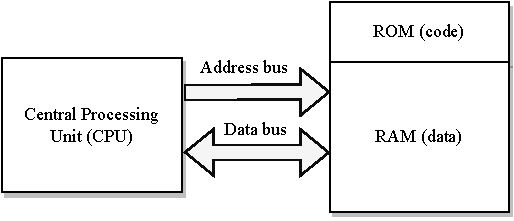
\includegraphics[width=.56\textwidth]{img/diagrams/von_neumann.pdf}
		\caption{Von Neumann architecture}
		\label{Von Neumann architecture}
	\end{figure}
	
	Another potential drawback arises from the fact that data and instructions share the same bus, even though fetching instructions occurs more frequently than data transfers. Consequently, the shared data bus may represent a performance bottleneck within the entire system.
	
	\subsubsection{Harvard Architecture}
	
	As shown in Figure \ref{Harvard architecture}, the Harvard architecture employs \textbf{distinct memory modules for code and data}, requiring twice the number of bus lines compared to the Von Neumann architecture \cite{harvard-architecture-1}. This design is typically preferred in scenarios where the performance benefits outweigh the additional costs, such as in microcontrollers, and \textit{Field Programmable Gate Arrays}, also known as \texttt{FPGA} boards.
	
	\begin{figure}[ht]
		\centering
		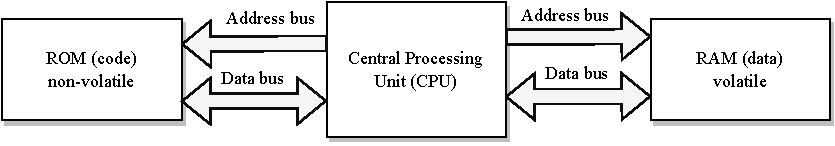
\includegraphics[width=.9\textwidth]{img/diagrams/harvard.pdf}
		\caption{Harvard architecture}
		\label{Harvard architecture}
	\end{figure}
	
	Taking advantage of two separate memory modules, it can effectively mitigate resource conflicts and enhance its performance through parallelism and separate memory caching.
	
	\subsection{Instruction Set Architectures}
	
	Instruction set architectures can also by categorized by how they handle operands in terms of their interaction with memory. As noted previously, each approach may be beneficial for different types of applications.
	
	\subsubsection{Stack Architecture}
	
	The stack architecture, shown in Figure \ref{Stack architecture}, does not rely on the main memory to retrieve operands. Instead, the \texttt{CPU} maintains an internal stack, which serves as storage for operands. An operation is executed in a \textit{last-in-first-out} (\texttt{LIFO}) fashion, where two operands are first popped off the stack, and the operation's result is consequently pushed back onto it \cite{computer-architecture-1}.
	
	\begin{figure}[ht]
		\centering
		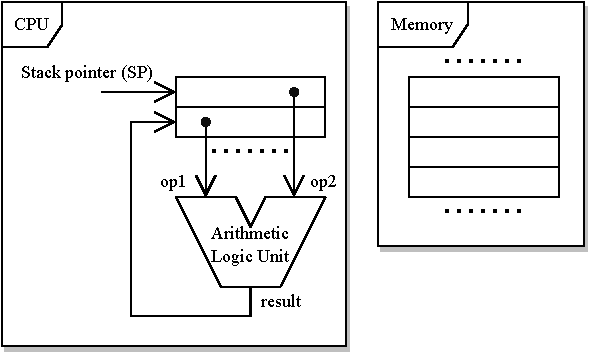
\includegraphics[width=.6\textwidth]{img/diagrams/stack_architecture.pdf}
		\caption{Stack architecture}
		\label{Stack architecture}
	\end{figure}
	
	A distinct advantage of this architecture is that it makes compiler implementation considerably easier compared to other types of architectures. However, the main drawback is the stack itself, which introduces a bottleneck that hinders any potential parallelization. This architectural design is employed, for example, by the Java Virtual Machine.
	
	\subsubsection{Accumulator Architecture}
	
	Similar to the stack architecture, the accumulator architecture, illustrated in Figure \ref{Accumulator architecture}, imposes minimal hardware requirements. It substitutes the stack with a single register called the accumulator, which serves both as an input operand and as storage for the operation's result. Same as the previous architecture, the accumulator represents a potential bottleneck. Furthermore, it leads to high memory traffic, as every two-operand instruction requires the second operand to be retrieved from memory. Some processor architectures are equipped with more than one accumulator. For instance, the MOS Technology 6502 microprocessor utilized in the \break Apple II computer featured not only a primary accumulator but also two index registers that functioned as additional accumulators \cite{computer-architecture-1}.
	
	\begin{figure}[ht]
		\centering
		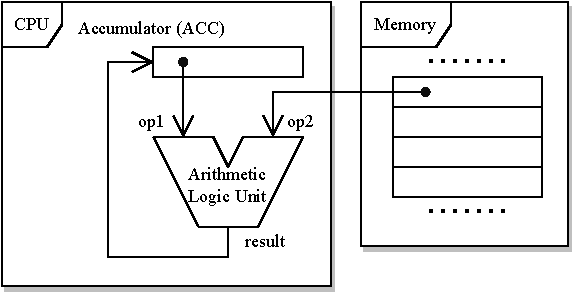
\includegraphics[width=.6\textwidth]{img/diagrams/accumulator_architecture.pdf}
		\caption{Accumulator architecture}
		\label{Accumulator architecture}
	\end{figure}
	
	\subsubsection{Load-Store Architecture} 
	
	Examining Figure \ref{Load-store architecture}, it can be observed that the load-store architecture does not utilize memory during arithmetic-logic operations. Instead, \textbf{it restricts memory access to a specific pair of instructions - the load and store instructions}, which serve as an interface for reading and writing data to memory. As a result, when an operation needs to be executed, the \texttt{CPU} must ensure that all operands are stored in individually addressable memory banks, known as \texttt{CPU} registers, before employing the arithmetic-logic unit, or \texttt{ALU}, to proceed with the operation \cite{computer-architecture-1}.
	
	\begin{figure}[ht]
		\centering
		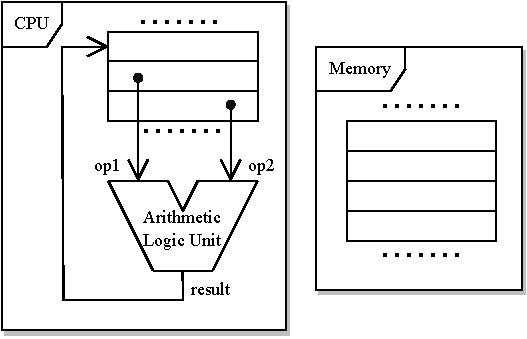
\includegraphics[width=.58\textwidth]{img/diagrams/load_store_architecture.pdf}
		\caption{Load-store architecture}
		\label{Load-store architecture}
	\end{figure}
	
	Figure \ref{Load-store sequence diagram} illustrates the process of retrieving operands from memory, carrying out the necessary operation, and consequently storing the result back in the main memory.
	
	Load-store architectures frequently use fixed-length instructions, providing the potential for more efficient pipelining \footnote{Pipelining is a low-level parallelization technique that involves breaking down the processing of an instruction into multiple stages that can be executed simultaneously.}, which can result in improved \break performance \cite{arm-soc}. However, a notable drawback of this architecture is its strong reliance on a sophisticated compiler, which may not be as straightforward to implement as in the architectures mentioned previously.
	
	\begin{figure}[ht]
		\centering
		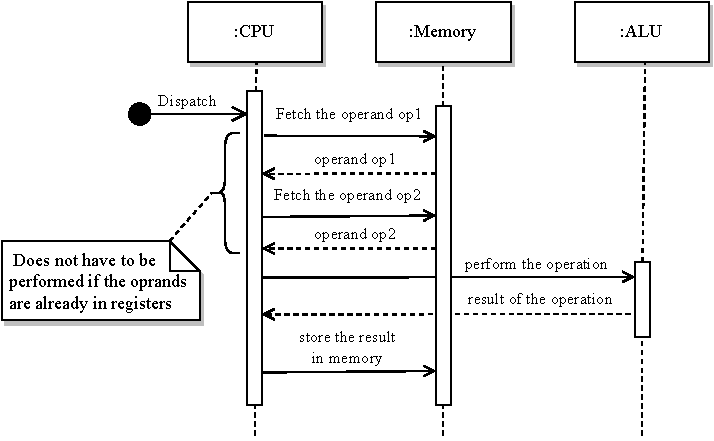
\includegraphics[width=.82\textwidth]{img/diagrams/load_store_sequence_diagram.pdf}
		\caption{Load-store sequence diagram}
		\label{Load-store sequence diagram}
	\end{figure}
	
	\subsection{Instruction Set Classification}
	
	\texttt{RISC}, which stands for \textit{Reduced Instruction Set Computer}, and \texttt{CISC}, or \textit{Complex Instruction Set Computer}, are two prominent \texttt{CPU} architectures that have gained widespread adoption over time. They employ distinct approaches in utilizing their respective instruction sets to align with the hardware implementation \cite{RISC-vs-CISC}.
	
	\subsubsection{Complex Instruction Set Computer}
	
	The \texttt{CISC} architecture places an \textbf{emphasis on the underlying hardware}, leading to the development of complex, usually multi-clock, instructions that can vary in length. This length variation may introduce complications in pipelining, which can have an adverse effect on performance. However, implementing custom instructions tailored to specific hardware specification results in smaller code sizes, as they take a more concrete and less abstract approach to achieve the desired functionality. An example of this type of architecture is the x86-64 Intel processor.
	
	\subsubsection{Reduced Instruction Set Computer}
	
	\texttt{RISC}, on the other hand, \textbf{focuses on the software aspect}, resulting in fewer single-clock instructions of a fixed-size, which facilitate easier pipeline processing. Another significant aspect is that \texttt{RISC} does not perform operations directly on memory. Instead, it adheres to the principle illustrated previously in Figure \ref{Load-store sequence diagram}. As depicted in Figure \ref{Comparison between the RISC and CISC architectures} below, another important consideration in this architecture is that having more general and, perhaps, simpler instructions can potentially increase the size of the final binary. This is due to the fact that, in \texttt{RISC}, achieving a specific function might involve using multiple instructions, whereas the \texttt{CISC} architecture usually accomplishes the same goal with a single instruction. An example of this architecture is the ARM architecture, which is described more in detail in Chapter~\ref{chapter-ARM Architecture}.
	
	\begin{figure}[ht]
		\centering
		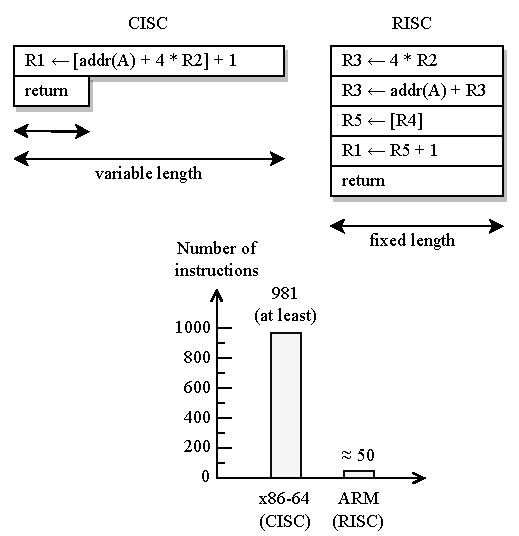
\includegraphics[width=0.70\textwidth]{img/diagrams/risc_vs_cisc.pdf}
		\caption{Comparison between the \texttt{RISC} and \texttt{CISC} architectures \cite{x86-vs-ARM}}
		\label{Comparison between the RISC and CISC architectures}
	\end{figure}
	
	\begin{important}
		There are other types of computer architectures that can be categorized by various aspects. The objective of this chapter was to provide the reader with introductory insights into some of the key factors that define a computer architecture. For more comprehensive information, the reader can refer, for instance, to the book series \textit{Computer Organization and Design: The Hardware/Software Interface} \cite{computer-organization-and-design}.
	\end{important}
	
	\chapter{ARM Architecture} \label{chapter-ARM Architecture}
	
	\section{History}
	
	ARM was officially founded as a company in November 1990 under the name \break Advanced RISC Machines Ltd. It originated as a joint venture involving companies such as Arcon Computers, Apple Computer, and VLSI Technology. Its early indications of future potential became evident with the Nokia 6110 GSM mobile, which experienced a remarkable surge in popularity after its release in 1998. Currently, it is estimated that over 99\% of the world's smartphones are built on ARM \break technology \cite{ARM-history}.
	
	Throughout the 2000s, ARM's sustained success enabled it to evolve beyond smartphones and become \textbf{arguably the most widely used processor architecture}. Nowadays, as illustrated in Figure \ref{Devices leveraging ARM technology}, ARM technology can be found across a broad spectrum of embedded devices, ranging from sensors and low-power microcontrollers to supercomputers and real-time mission-critical systems \cite{ARM-history}.
	
	\begin{figure}[ht]
		\centering
		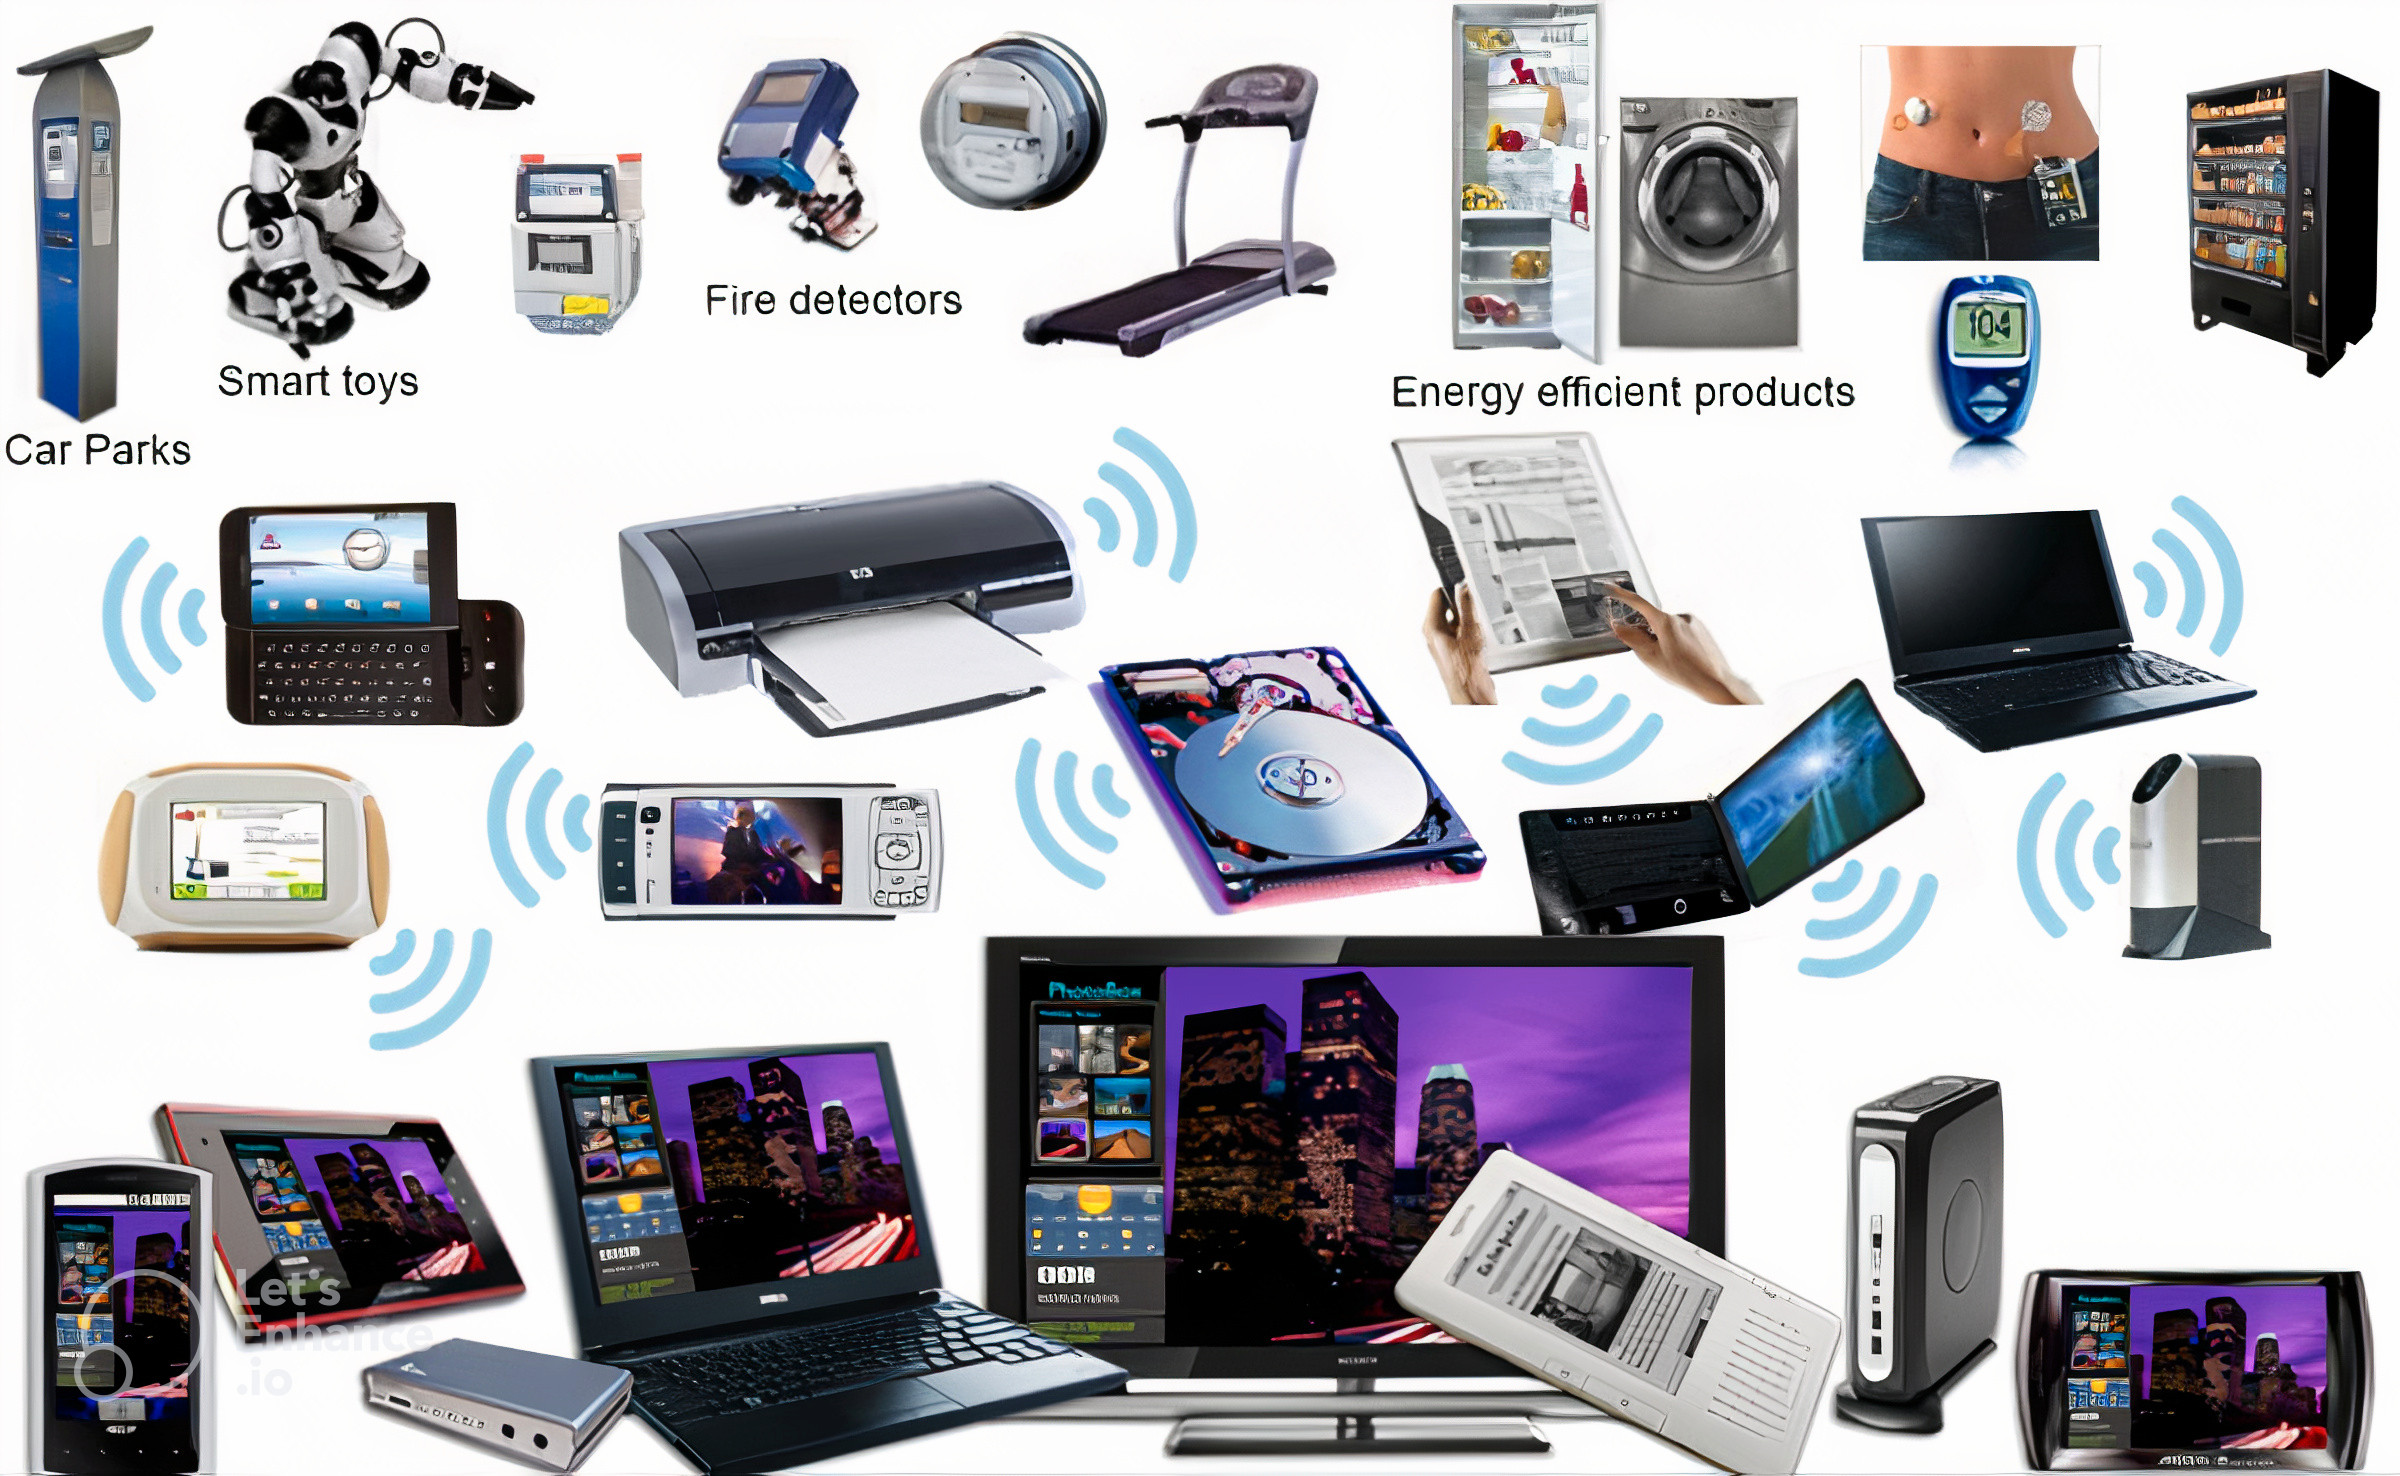
\includegraphics[width=0.65\textwidth]{img/diagrams/arm_powered_products.jpg}
		\caption{Devices leveraging ARM technology}
		\label{Devices leveraging ARM technology}
	\end{figure}
	
	An interesting aspect of ARM is that \textbf{it does not engage in silicon manufacturing}. Instead, it preserves the architecture as intellectual property, outsourcing the implementation to its closely aligned silicon partners, who are part of the so-called \textit{Connected Community}. This ARM surrounding community forms a global network of companies that collaborate by sharing expertise, providing support services, offering design consulting, and supplying tools for creating ARM-powered solutions.
	
	\section{Processor Cores}
	
	\textbf{ARM classifies its processors into three major groups}, which makes it a viable choice for a wide range of applications. Figure \ref{ARM processor roadmap} displays these categories in ascending order based on their capabilities.
	
	\begin{figure}[ht]
		\centering
		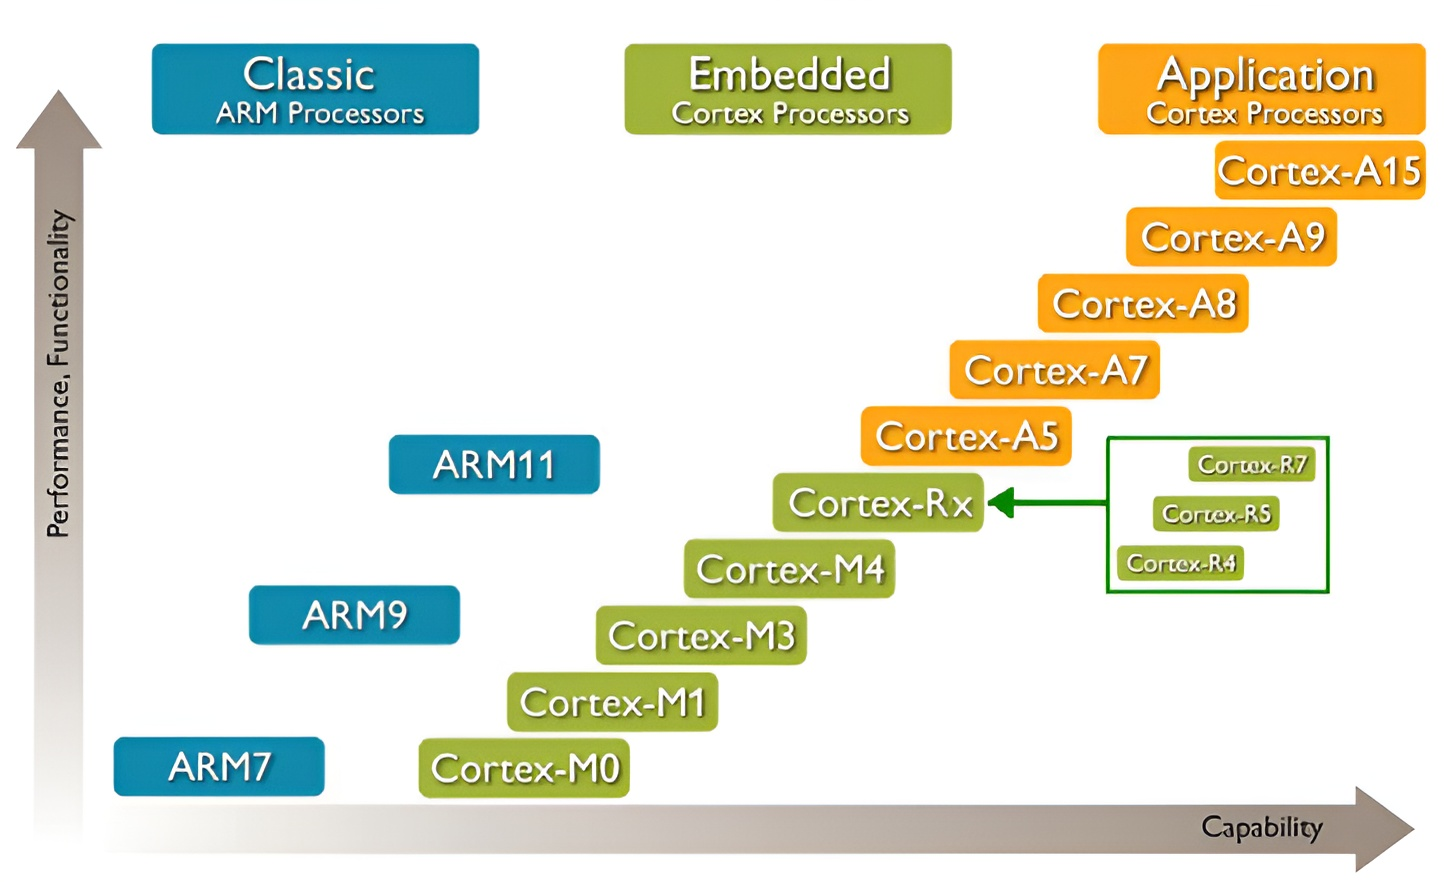
\includegraphics[width=0.8\textwidth]{img/diagrams/arm_processor_roadmap.jpeg}
		\caption{ARM processor roadmap}
		\label{ARM processor roadmap}
	\end{figure}
	
	\subsection{Classic ARM Processors}
	
	The Classic ARM Processors represent the company's \textbf{initial line of processors}. A typical example within this category is the \texttt{ARM7TDMI-S} \texttt{CPU} core, which was widely embraced by the cellphone industry \cite{ARM-mobile}. Over time, ARM has introduced additional Cortex families, each tailored for their intended domain of applications.
	
	\subsection{Embedded Cortex Processors}
	
	Generally speaking, the Cortex-M family is utilized in \textbf{low-cost microcontrollers}, which can be commonly found embedded in Internet of Things, or \texttt{IoT}, devices such as home automation systems, wearables\footnote{Wearable technology refers to any type of smart devices designed to be worn, such as smartwatches, smart glasses, etc.}, or smart locks.
	
	\begin{important}
		Usually, the ARM Cortex-M family simplifies or modifies certain features, resulting in slight deviations from the traditional ARM architecture. These modifications may involve different \texttt{CPU} modes, the exception model, or bank registers, all of which are further discussed in the following sections.
	\end{important}
	
	Another line of processors targeted for the embedded world is the Cortex-R family, known for delivering high performance and throughput while upholding precise timing properties and minimizing interrupt latency. This characteristic makes it a \textbf{suitable core for domains with time-constrained requirements}, including automotive systems, medical devices, aerospace, defense, and real-time systems.
	
	\subsection{Application Cortex Processors}
	
	The Cortex-A line of processors is designed for applications that require a general-purpose platform operating system, which is \textbf{commonly used in laptops and personal computers}. As a result, they integrate an extended instruction set to improve multimedia processing, along with an advanced memory management system to ensure a seamless human-machine interaction experience.
	
	\begin{figure}[ht]
		\centering
		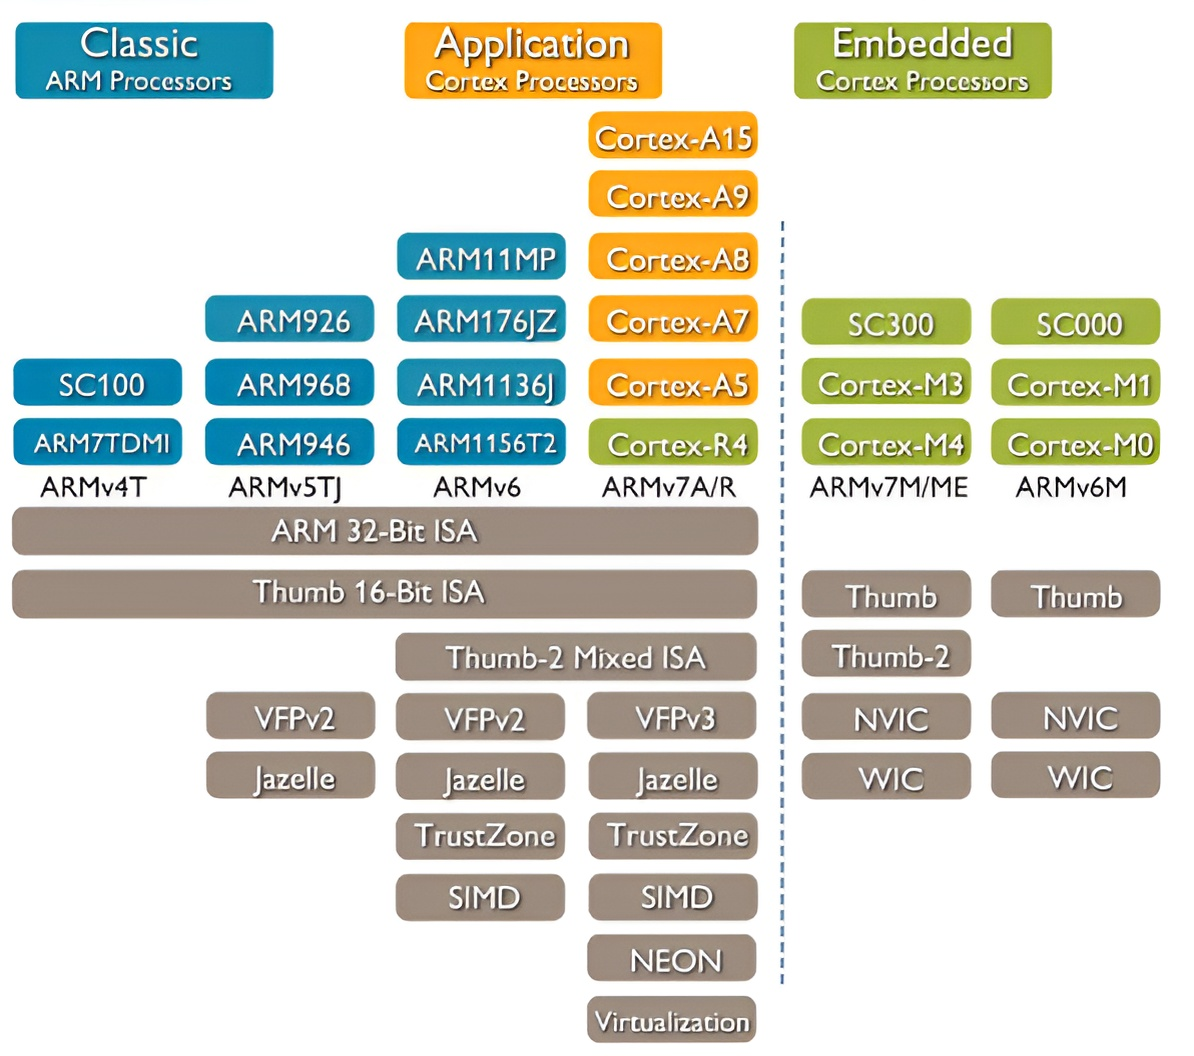
\includegraphics[width=0.8\textwidth]{img/diagrams/arm_processor_roadmap2.jpeg}
		\caption{Features of different ARM processor cores}
		\label{Features of different ARM processor cores}
	\end{figure}
	
	Figure \ref{Features of different ARM processor cores} illustrates the ongoing evolution of capability features across various \texttt{CPU} cores.
	
	\newpage
	
	For instance, it can be observed that ARMv6 incorporates the \textit{Thumb} instruction set version 2, which is runtime interchangeable with the \textit{ARM} instruction set. Additionally, it includes support for floating-point operations version 2, \textit{Jazelle} for execution of \texttt{Java bytecode}, \textit{TrustZone} for secure data storage, and \textit{Single Instruction/Multiple Data} instructions, often referred to as \texttt{SIMD} instructions.
	
	\section{Instruction Set Architecture}
	
	As mentioned in Section \ref{Classification of Computer Architectures}, \textbf{ARM is a load-store \texttt{RISC} architecture} that supports two major sets of fixed-size instructions - the standard 32-bit \textit{ARM} instruction set and the reduced 16-bit \textit{Thumb} instruction set. The following sections delve into some of the key characteristics of the Classic line of ARM processors. For a more comprehensive understanding, the reader is encouraged to refer to the official ARM Architecture Reference Manual \cite{ARM_reference_manual}.
	
	\subsection{Central Processing Unit Modes}
	
	There are a total of \textbf{seven modes in which a modern ARM \texttt{CPU} can operate}, each represented by a unique 5-bit number stored in the \textit{Current Program Status Register}. The \texttt{CPU} can switch to one of these modes either implicitly, such as when an interrupt occurs, or explicitly as intended by the programmer, for example, when switching the current \texttt{CPU} context. All modes except for the \textit{User} mode are privileged, meaning that when the \texttt{CPU} is in the unprivileged mode, the execution of certain instructions might be restricted \footnote{In the context of operating systems, a non-privileged mode is typically used for the execution of user programs, while the kernel operates in a privileged mode.}. Table \ref{List of ARM CPU modes} summarizes all available \texttt{CPU} modes.
	
	\begin{center}
		\begin{longtable}{p{.16\textwidth}p{.70\textwidth}}
			\caption{List of ARM \texttt{CPU} modes}
			\label{List of ARM CPU modes}\\
			\toprule[1.5pt]
			\textbf{\texttt{CPU} mode} & \textbf{Description}\\
			\midrule
			\endfirsthead
			\multicolumn{2}{c}{\tablename{}~\thetable{} \textit{(continued from the previous page)}}\\
			\midrule
			\textbf{Bit position} & \textbf{Description}\\
			\midrule
			\endhead
			\midrule
			\multicolumn{2}{r}{\textit{(table continues on the next page)}}\\
			\endfoot
			\bottomrule[1.5pt]
			\endlastfoot
			%
			\textit{User} & Normal program execution\\
			\textit{FIQ} & Supports a high-speed data transfer or channel process\\
			\textit{IRQ} & Used for general-purpose interrupt handling\\
			\textit{Supervisor} & A protected mode for the operating system\\
			\textit{Abort} & Implements virtual memory and/or memory protection\\
			\textit{Undefined} & Supports software emulation of hardware co-processors\\
			\textit{System} & Runs privileged operating system tasks\\
		\end{longtable}
	\end{center}
	
	\begin{important}
		It is worth noting that Cortex-M utilizes only two \texttt{CPU} modes - \textit{Thread} mode, an unprivileged mode designed for executing application code, and \textit{Handler} mode, a privileged mode intended for handling exceptions.
	\end{important}
	
	\subsection{Exception Model}
	
	When an exception or interrupt occurs, the \texttt{CPU} sets the \textit{Program Counter Register}, or \texttt{PC} for short, to the address associated with that exception, known as the interrupt vector, and switches to the corresponding \texttt{CPU} mode, which can be found in Table \ref{List of ARM CPU exceptions}. The interrupt vector represents a fixed address in \texttt{RAM} where the \texttt{CPU} redirects its execution. Therefore, during the system initialization, these memory locations are typically filled with branch instructions to direct the execution to the corresponding exception handlers.
	
	As illustrated in Figure \ref{Possible locations of the interrupt vector table in RAM}, this address region, also known as the interrupt vector table, or \texttt{IVT}, can be found located either in the lower part or the upper part of the virtual address space, depending on the current setting stored in the \textit{System Control Co-processor}. In practice, the lower part of the address space is usually reserved for user processes, while the kernel is remapped to the upper part, hence the option to relocate the \texttt{IVT} as well \footnote{In the ARM architecture, the lower portion of the address space is typically controlled by \textit{Translation Table 0}, with its address is stored in the \texttt{TTBR0} register. Simultaneously, the kernel section is managed in parallel by \textit{Translation Table 1}, whose address is located in the \texttt{TTBR1} register. From the viewpoint of an operating system, the presence of two distinct page tables provides the advantage of avoiding the need to replicate kernel pages for each individual process created.}.
	
	\begin{figure}[ht]
		\centering
		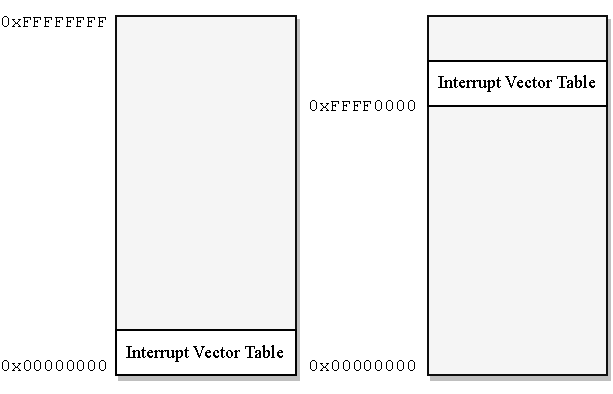
\includegraphics[width=0.7\textwidth]{img/diagrams/ivt_location.pdf}
		\caption{Possible locations of the interrupt vector table in \texttt{RAM}}
		\label{Possible locations of the interrupt vector table in RAM}
	\end{figure}
	
	Table \ref{List of ARM CPU exceptions} provides a list of addresses for individual vectors located in both the lower and upper portions of the address space.
	
	\newpage
	
	\begin{center}
		\begin{longtable}{p{.25\textwidth}p{.14\textwidth}p{.25\textwidth}p{.22\textwidth}}
			\caption{List of ARM \texttt{CPU} exceptions}
			\label{List of ARM CPU exceptions}\\
			\toprule[1.5pt]
			\textbf{Exception} & \textbf{CPU mode} & \textbf{Normal address} & \textbf{High address}\\
			\midrule
			\endfirsthead
			\multicolumn{3}{c}{\tablename{}~\thetable{} \textit{(continued from the previous page)}}\\
			\midrule
			\textbf{Exception} & \textbf{CPU mode} & \textbf{Normal address} & \textbf{High address}\\
			\midrule
			\endhead
			\midrule
			\multicolumn{3}{r}{\textit{(table continues on the next page)}}\\
			\endfoot
			\bottomrule[1.5pt]
			\endlastfoot
			%
			\textit{Reset} & \textit{Supervisor} & \texttt{0x00000000} & \texttt{0xFFFF0000}\\
			\textit{Undefined instruction} & \textit{Undefined} & \texttt{0x00000004} & \texttt{0xFFFF0004}\\
			\textit{Software interrupt} & \textit{Supervisor} & \texttt{0x00000008} & \texttt{0xFFFF0008}\\
			\textit{Prefetch abort} & \textit{Abort} & \texttt{0x0000000C} & \texttt{0xFFFF000C}\\
			\textit{Data abort} & \textit{Abort} & \texttt{0x00000010} & \texttt{0xFFFF0010}\\
			\textit{Interrupt} & \textit{IRQ} & \texttt{0x00000018} & \texttt{0xFFFF0018}\\
			\textit{Fast interrupt} & \textit{FIQ} & \texttt{0x0000001C} & \texttt{0xFFFF001C}\\
		\end{longtable}
	\end{center}
	
	\begin{important}
		Similar to the previously mentioned \texttt{CPU} modes, the Cortex-M family employs a slightly different exception model, specifically tailored for microcontroller applications.
	\end{important}
	
	\subsection{Registers}
	
	ARM offers \textbf{16 general-purpose 32-bit registers} labeled \texttt{r0} through \texttt{r15}, three of which serve special functions, which are listed in Table \ref{List of special function ARM registers}. The programmer is free to use the remaining registers as needed.
	
	However, specific calling conventions were established to ensure a systematic use of these registers. For instance, registers \texttt{r0-r3} are used as argument values passed into a subroutine, while return values are typically stored in registers \texttt{r0-r1}. Further details on calling conventions can be found in Chapter 6 of the ARM's Procedure Call Standard Manual \cite{ARM-calling-conventions}.
	
	\begin{center}
		\begin{longtable}{p{.10\textwidth}p{.15\textwidth}p{.65\textwidth}}
			\caption{List of special function ARM registers}
			\label{List of special function ARM registers}\\
			\toprule[1.5pt]
			\textbf{Index} & \textbf{Mnemonic} & \textbf{Description}\\
			\midrule
			\endfirsthead
			\multicolumn{3}{c}{\tablename{}~\thetable{} \textit{(continued from the previous page)}}\\
			\midrule
			\textbf{Mnemonic} & \textbf{Description}\\
			\midrule
			\endhead
			\midrule
			\multicolumn{3}{r}{\textit{(table continues on the next page)}}\\
			\endfoot
			\bottomrule[1.5pt]
			\endlastfoot
			%
			\texttt{13} & \texttt{SP} & \textit{Stack pointer} - holds the address of the top of the stack \\
			\texttt{14} & \texttt{LR} & \textit{Link register} - holds the return address (when calling a function, it is not pushed onto the stack)\\ 
			\texttt{15} & \texttt{PC} & \textit{Program counter} - holds the address of the instruction to be executed \\
		\end{longtable}
	\end{center}
	
	\subsubsection{Banked Registers} \label{section-banked-registers}
	
	A distinctive feature of ARM is its utilization of so-called \textit{bank} registers. In this concept, \textbf{the majority of \texttt{CPU} modes have their own unique set of registers} that are automatically loaded whenever the current \texttt{CPU} mode changes.
	
	The more bank registers are utilized, the faster the switch into the corresponding \texttt{CPU} mode is, as there is no need to preserve the current state by storing all registers onto the stack. As a result, this concept is extensively employed by the \textit{FIQ} mode for ensuring fast interrupt handling, hence the mode's name.
	
	Figure \ref{Bank registers of different CPU modes} displays distinct bank registers for each \texttt{CPU} mode. Notably, \textit{User}, the unprivileged mode, and \textit{System}, a privileged mode, utilize the same set of underlying registers, which serves as a \say{meeting point} between the kernel and user space when, for instance, running system tasks or handling system calls.
	
	\begin{figure}[ht]
		\centering
		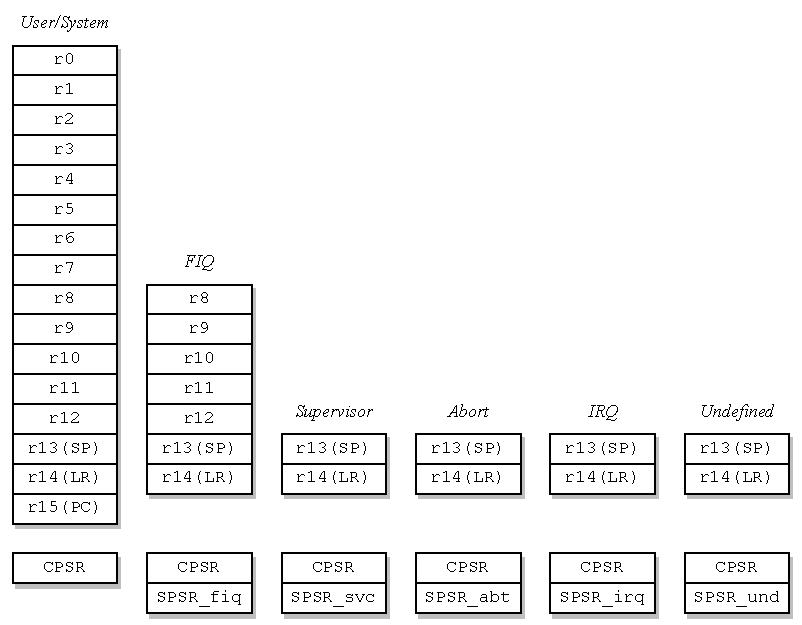
\includegraphics[width=0.98\textwidth]{img/diagrams/bank_registers_2.pdf}
		\caption{Bank registers of different \texttt{CPU} modes}
		\label{Bank registers of different CPU modes}
	\end{figure}
	
	When the \texttt{CPU} is executing 16-bit \textit{Thumb} instructions, only the first 8 registers (\texttt{r0-r7}) can be addressed directly. These registers are sometimes referred to as the \textit{Thumb State Low Registers}.
	
	\newpage
	
	\begin{important}
		As far as Cortex-M is concerned, since there are only two \texttt{CPU} modes, the banking scheme applies only to the \texttt{SP} register.
	\end{important}
	
	\subsubsection{Control Registers}
	
	In general, control registers are \textbf{specialized registers within a processor that are used to manage system configuration}, memory, interrupts, and power. They enable software to interact with and configure hardware features, such as system-wide settings and power-saving mechanisms.
	
	\paragraph{Current Program Status Register}
	
	The \texttt{CPSR} register, which stands for \textit{Current Program Status Register}, \textbf{preserves the current state of the \texttt{CPU}} along with some additional information. To modify the control register, its content must first be transferred into one of the general-purpose registers using the \texttt{MRS} instruction, as its direct modification is not permitted. Subsequently, after the necessary modifications have been made, it can be transferred back from the general-purpose register using the \texttt{MSR} instruction.
	
	This 32-bit register is segmented into four sections, as illustrated in Figure \ref{Current Program Status Register}. The initial letters of the section names (\texttt{F}, \texttt{S}, \texttt{E}, and \texttt{C}) can function as a bit mask when using the \texttt{MRS} or \texttt{MSR} instruction to prevent unintentional modifications of bits that are not meant to be changed.
	
	\begin{figure}[ht]
		\centering
		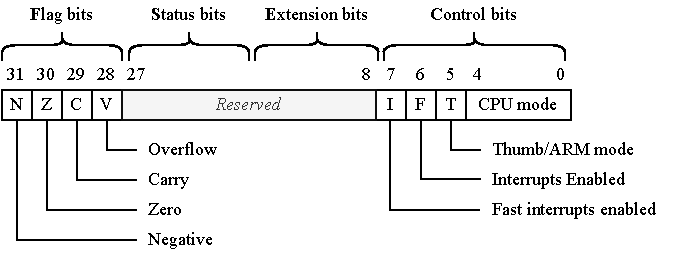
\includegraphics[width=0.85\textwidth]{img/diagrams/cpsr.pdf}
		\caption{Current Program Status Register\protect\footnotemark}
		\label{Current Program Status Register}
	\end{figure}
	
	\footnotetext{The reserved area contains additional information and control bits including the result of \texttt{SIMD} instructions, the status of the Jazelle bit, and endianness, which can also be changed at runtime.}
	
	\paragraph{Saved Program Status Register}
	
	The \textit{Saved Program Status Register}, or \texttt{SPSR}, serves as a \textbf{copy of the \texttt{CPSR} register} utilized during \texttt{CPU} mode switching. When transitioning to a mode that contains an \texttt{SPSR} register, as shown in Figure \ref{Bank registers of different CPU modes}, the contents of the \texttt{CPSR} register of the current mode are copied into the \texttt{SPSR} register of the target mode. 
	
	This process allows a future restoration of the original state when reverting to the original \texttt{CPU} mode.
	
	\subsection{ARM Instructions}
	
	As mentioned previously, \textbf{all instructions in the \textit{ARM} instruction set are 32-bits in length}. As shown in Figure \ref{Condition field of an ARM instruction}, the most significant four bits of each instruction form a condition filed that constrains its execution. The \texttt{CPU} assesses the current state of the flag bits in the \texttt{CPSR} register, and depending on the condition field, the instruction is either skipped or executed. From the programmer's standpoint, this can be accomplished by suffixing the instruction name by the desired condition code, as listed in Table \ref{List of ARM instruction condition codes}.
	
	In contrast to other architectures, the flag bits are not automatically set upon the execution of an instruction. Instead, it is up to the programmer to choose whether to update them by appending an \texttt{'S'} to the instruction name. For instance, the \texttt{ADD} instruction does not update the flags, whereas \texttt{ADDS} does \footnote{This concept does not apply to instructions like \texttt{CMP}, which, as its sole purpose suggests, implicitly sets the status flags.}.
	
	\begin{figure}[ht]
		\centering
		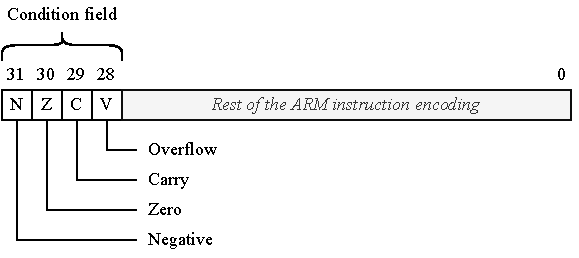
\includegraphics[width=0.74\textwidth]{img/diagrams/condition_field.pdf}
		\caption{Condition field of an ARM instruction}
		\label{Condition field of an ARM instruction}
	\end{figure}
	
	\newpage
	
	\begin{center}
		\begin{longtable}{p{.12\textwidth}p{.27\textwidth}p{.51\textwidth}}
			\caption{List of ARM instruction condition codes}
			\label{List of ARM instruction condition codes}\\
			\toprule[1.5pt]
			\textbf{Code} & \textbf{Flags tested} & \textbf{Meaning}\\
			\midrule
			\endfirsthead
			\multicolumn{3}{c}{\tablename{}~\thetable{} \textit{(continued from the previous page)}}\\
			\midrule
			\textbf{Code} & \textbf{Flags tested} & \textbf{Meaning}\\
			\midrule
			\endhead
			\midrule
			\multicolumn{3}{r}{\textit{(table continues on the next page)}}\\
			\endfoot
			\bottomrule[1.5pt]
			\endlastfoot
			%
			\texttt{EQ} & \texttt{Z==1} & Equal\\
			\texttt{NE} & \texttt{Z==0} & Not equal\\
			\texttt{CS} or \texttt{HS} & \texttt{C==1} & Unsigned higher or same (or carry set)\\
			\texttt{CC} or \texttt{LO} & \texttt{C==0} & Unsigned lower (or carry clear)\\
			\texttt{MI} & \texttt{N==1} & Negative (mnemonic - \say{minus})\\
			\texttt{PL} & \texttt{N==0} & Positive or zero (mnemonic - \say{plus})\\
			\texttt{VS} & \texttt{V==1} & Signed overflow (mnemonic - \say{\texttt{V} set})\\
			\texttt{VC} & \texttt{V==0} & No signed overflow (mnemonic - \say{\texttt{V} clear})\\
			\texttt{HI} & \texttt{(C==1) \&\& (Z==0)} & Unsigned higher\\
			\texttt{LS} & \texttt{(C==0) || (Z==1)} & Unsigned lower or same\\
			\texttt{GE} & \texttt{N==V} & Signed greater than or equal\\
			\texttt{LT} & \texttt{N!=V} & Signed less than\\
			\texttt{GT} & \texttt{(Z==0) \&\& (N==V)} & Signed greater than\\
			\texttt{LE} & \texttt{(Z==1) || (N!=V)} & Signed less than or equal\\
			\texttt{AL} & Not tested & Always executed (suffix is omitted)\\
		\end{longtable}
	\end{center}
	
	In general, \textbf{ARM instructions can be classified into several different categories based on their purposes}, such as \textit{data processing instructions}, \textit{data transfer instructions}, \textit{branch instructions}, or \textit{co-processor instructions}, which are designed for interacting with external \texttt{CPU} co-processors. Detailed ARMv6 instruction encodings can be found, for instance, in the B2 ARM Appendix document \cite{B2_appendix}.
	
	\section{Co-processors}
	
	As showcased in Figure \ref{Context of an ARM co-processor}, a co-processor, as its name implies, \textbf{operates alongside the main \texttt{CPU} to further extend its functionality}. Examples of co-processors may include a floating-point unit or the system control co-processor. Each co-processor is addressed by a unique 4-bit number \footnote{The co-processor \texttt{ID} is encoded in every co-processor instruction.}, resulting in up to 16 different co-processors that can be attached to an ARM \texttt{CPU}.
	
	As listed in Table \ref{List of ARM co-processor instructions}, the \textbf{\texttt{CPU} interacts with co-processors via three designated instructions}, enabling it to offload specific functions to more specialized hardware suitable for the given task, such as when multiplying two floating-point numbers.
	
	\begin{center}
		\begin{longtable}{p{.35\textwidth}p{.50\textwidth}}
			\caption{List of ARM co-processor instructions}
			\label{List of ARM co-processor instructions}\\
			\toprule[1.5pt]
			\textbf{Instruction} & \textbf{Description}\\
			\midrule
			\endfirsthead
			\multicolumn{2}{c}{\tablename{}~\thetable{} \textit{(continued from the previous page)}}\\
			\midrule
			\textbf{Instruction} & \textbf{Description}\\
			\midrule
			\endhead
			\midrule
			\multicolumn{2}{r}{\textit{(table continues on the next page)}}\\
			\endfoot
			\bottomrule[1.5pt]
			\endlastfoot
			%
			\textit{Coprocessor Data Operation}\newline(\texttt{CDP}) & Signals a co-processor to perform an internal operation\\
			\textit{Coprocessor Data Transfer}\newline(\texttt{LDC}, \texttt{STC}) & Loads or stores a subset of co-processor's registers directly to memory\\
			\textit{Coprocessor Register Transfer}\newline(\texttt{MRC}, \texttt{MCR}) & Communicates information directly between the \texttt{CPU} and a co-processor\\
		\end{longtable}
	\end{center}
	
	\begin{figure}[ht]
		\centering
		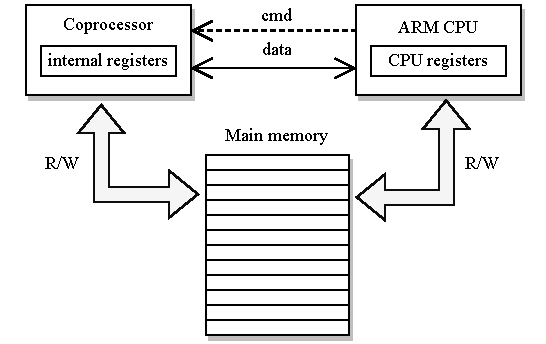
\includegraphics[width=0.78\textwidth]{img/diagrams/coprocessors_3.pdf}
		\caption{Context of an ARM co-processor}
		\label{Context of an ARM co-processor}
	\end{figure}
	
	\subsection{System Control Co-processor}
	
	The system control co-processor, or \texttt{CP15}, incorporates a tree-like structure of additional registers that are utilized for \textbf{configuring various settings within the overall system}. For instance, the users can configure branch prediction, caching, unaligned-memory access, paging, and so on. Moreover, via \texttt{CP15}, users can enable or disable other co-processors and define their \texttt{CPU} mode access rights.
	
	\subsection{Floating-point Unit}
	
	The floating-point unit, also referred to as the \texttt{FPU}, is represented by two distinct co-processors, \texttt{CP10} (single-precision) and \texttt{CP11} (double-precision). As illustrated in Figure \ref{Floating-point registers}, this distinction occurs solely  at an interface level, meaning that they share the same underlining set of registers, which are treated differently based on the leveraged co-processor. The primary purpose of the \texttt{FPU} is to extend the capability of an ARM \texttt{CPU} by \textbf{incorporating floating-point arithmetic instructions}, such as \textit{addition}, \textit{subtraction}, \textit{multiplication}, \textit{division}, and \textit{square root} operations.
	
	\begin{figure}[ht]
		\centering
		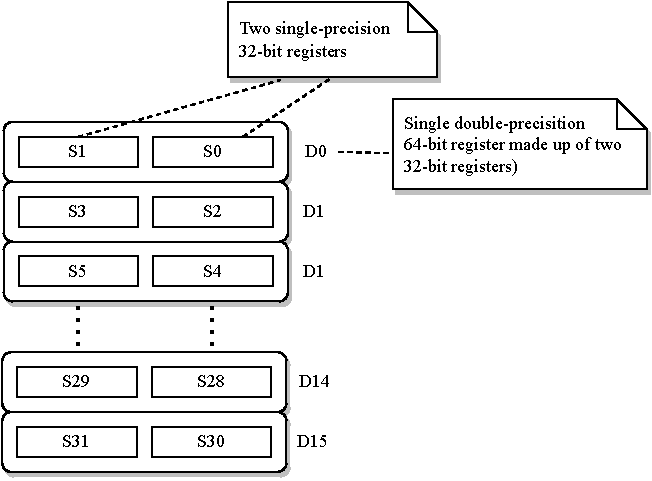
\includegraphics[width=0.8\textwidth]{img/diagrams/fpu_registers.pdf}
		\caption{Floating-point registers}
		\label{Floating-point registers}
	\end{figure}
	
	Additionally, the \texttt{FPU} also provides its own \textit{Status Control Register}, called \texttt{FPSCR}, which contains the current state of flags. Whenever a comparison instruction is executed, it becomes essential to transfer the \texttt{FPU} flags to the \texttt{CPU}, so they can be used to determine the execution of the next instruction \footnote{From the programmer's perspective, this process is typically automated by the compiler, which implicitly inserts a subsequent \texttt{MRC} instruction.}.
	
	Finally, the user can optionally set different rounding modes and exceptions via the \textit{Exception Control Register} named \texttt{FPEXC}. This register is also employed to activate the \texttt{FPU}. As a result, it must be initially enabled on a co-processor level (in \texttt{CP15}) and subsequently in the \texttt{FPEXC} register as well.
	
	\chapter{Raspberry Pi Zero}
	
	\textbf{Raspberry Pi Zero is a system on chip}, or \texttt{SoC}, which is a design that integrates various components into a single chip, such as a central and graphics processing unit, memory interfaces, and input-output devices. As far as Raspberry Pi Zero is concerned, it is equipped with 512 \texttt{MB} of \texttt{RAM}, an \texttt{SD} card holder, which is utilized during the booting process, a Mini \texttt{HDMI} adapter, a micro \texttt{USB} port, and the \texttt{BCM2835} microcontroller, which is powered by the \texttt{ARM1176JZF\_S} processor \cite{ARM1176JZF-S}. Figure \ref{Raspberry Pi Zero board} labels the main visual components of the board.
	
	\begin{figure}[ht]
		\centering
		% 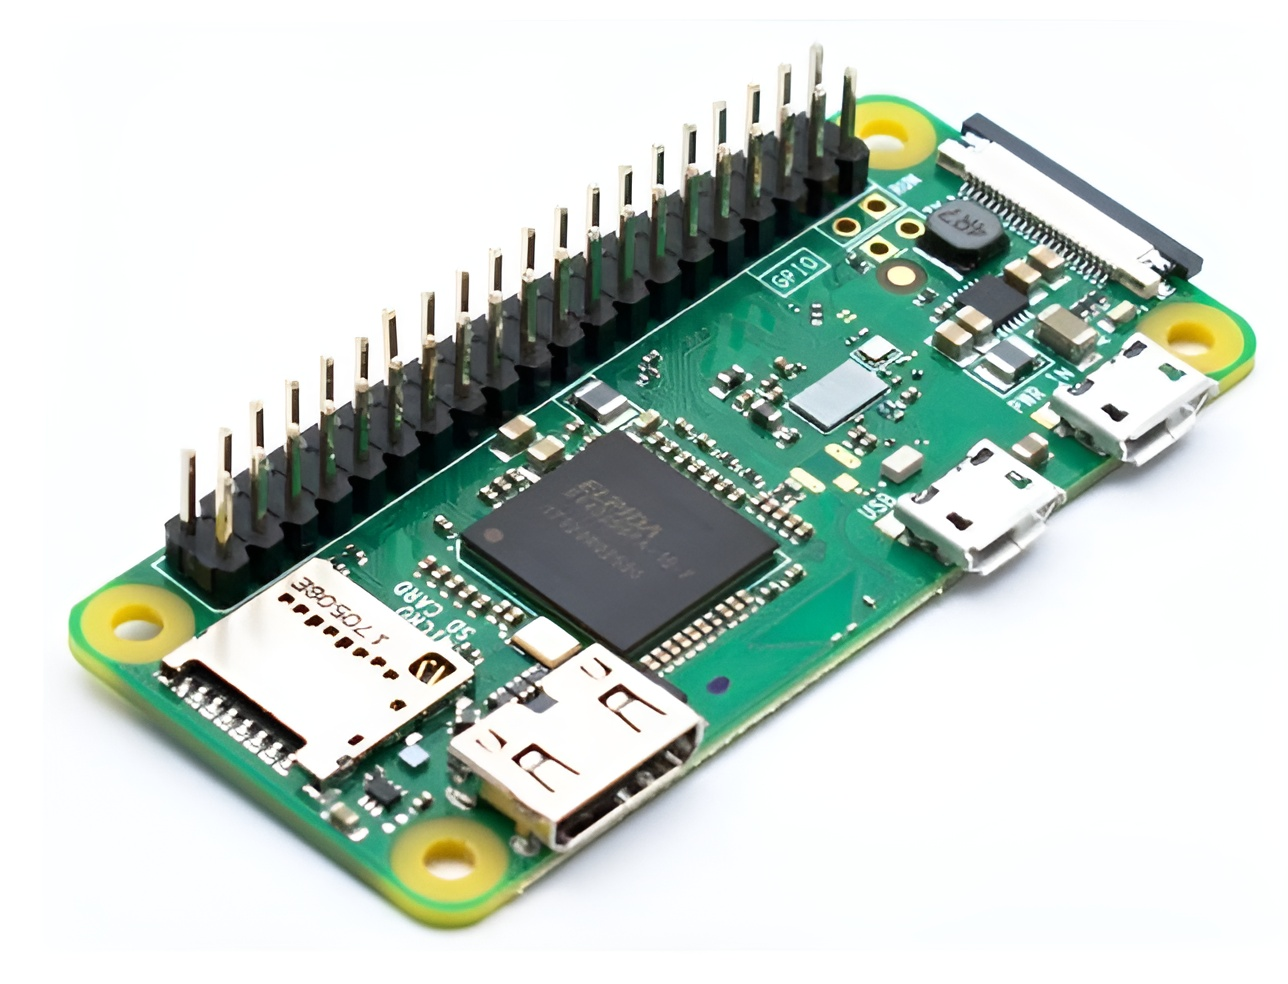
\includegraphics[width=0.4\textwidth]{img/diagrams/rpi_zero.jpeg}
		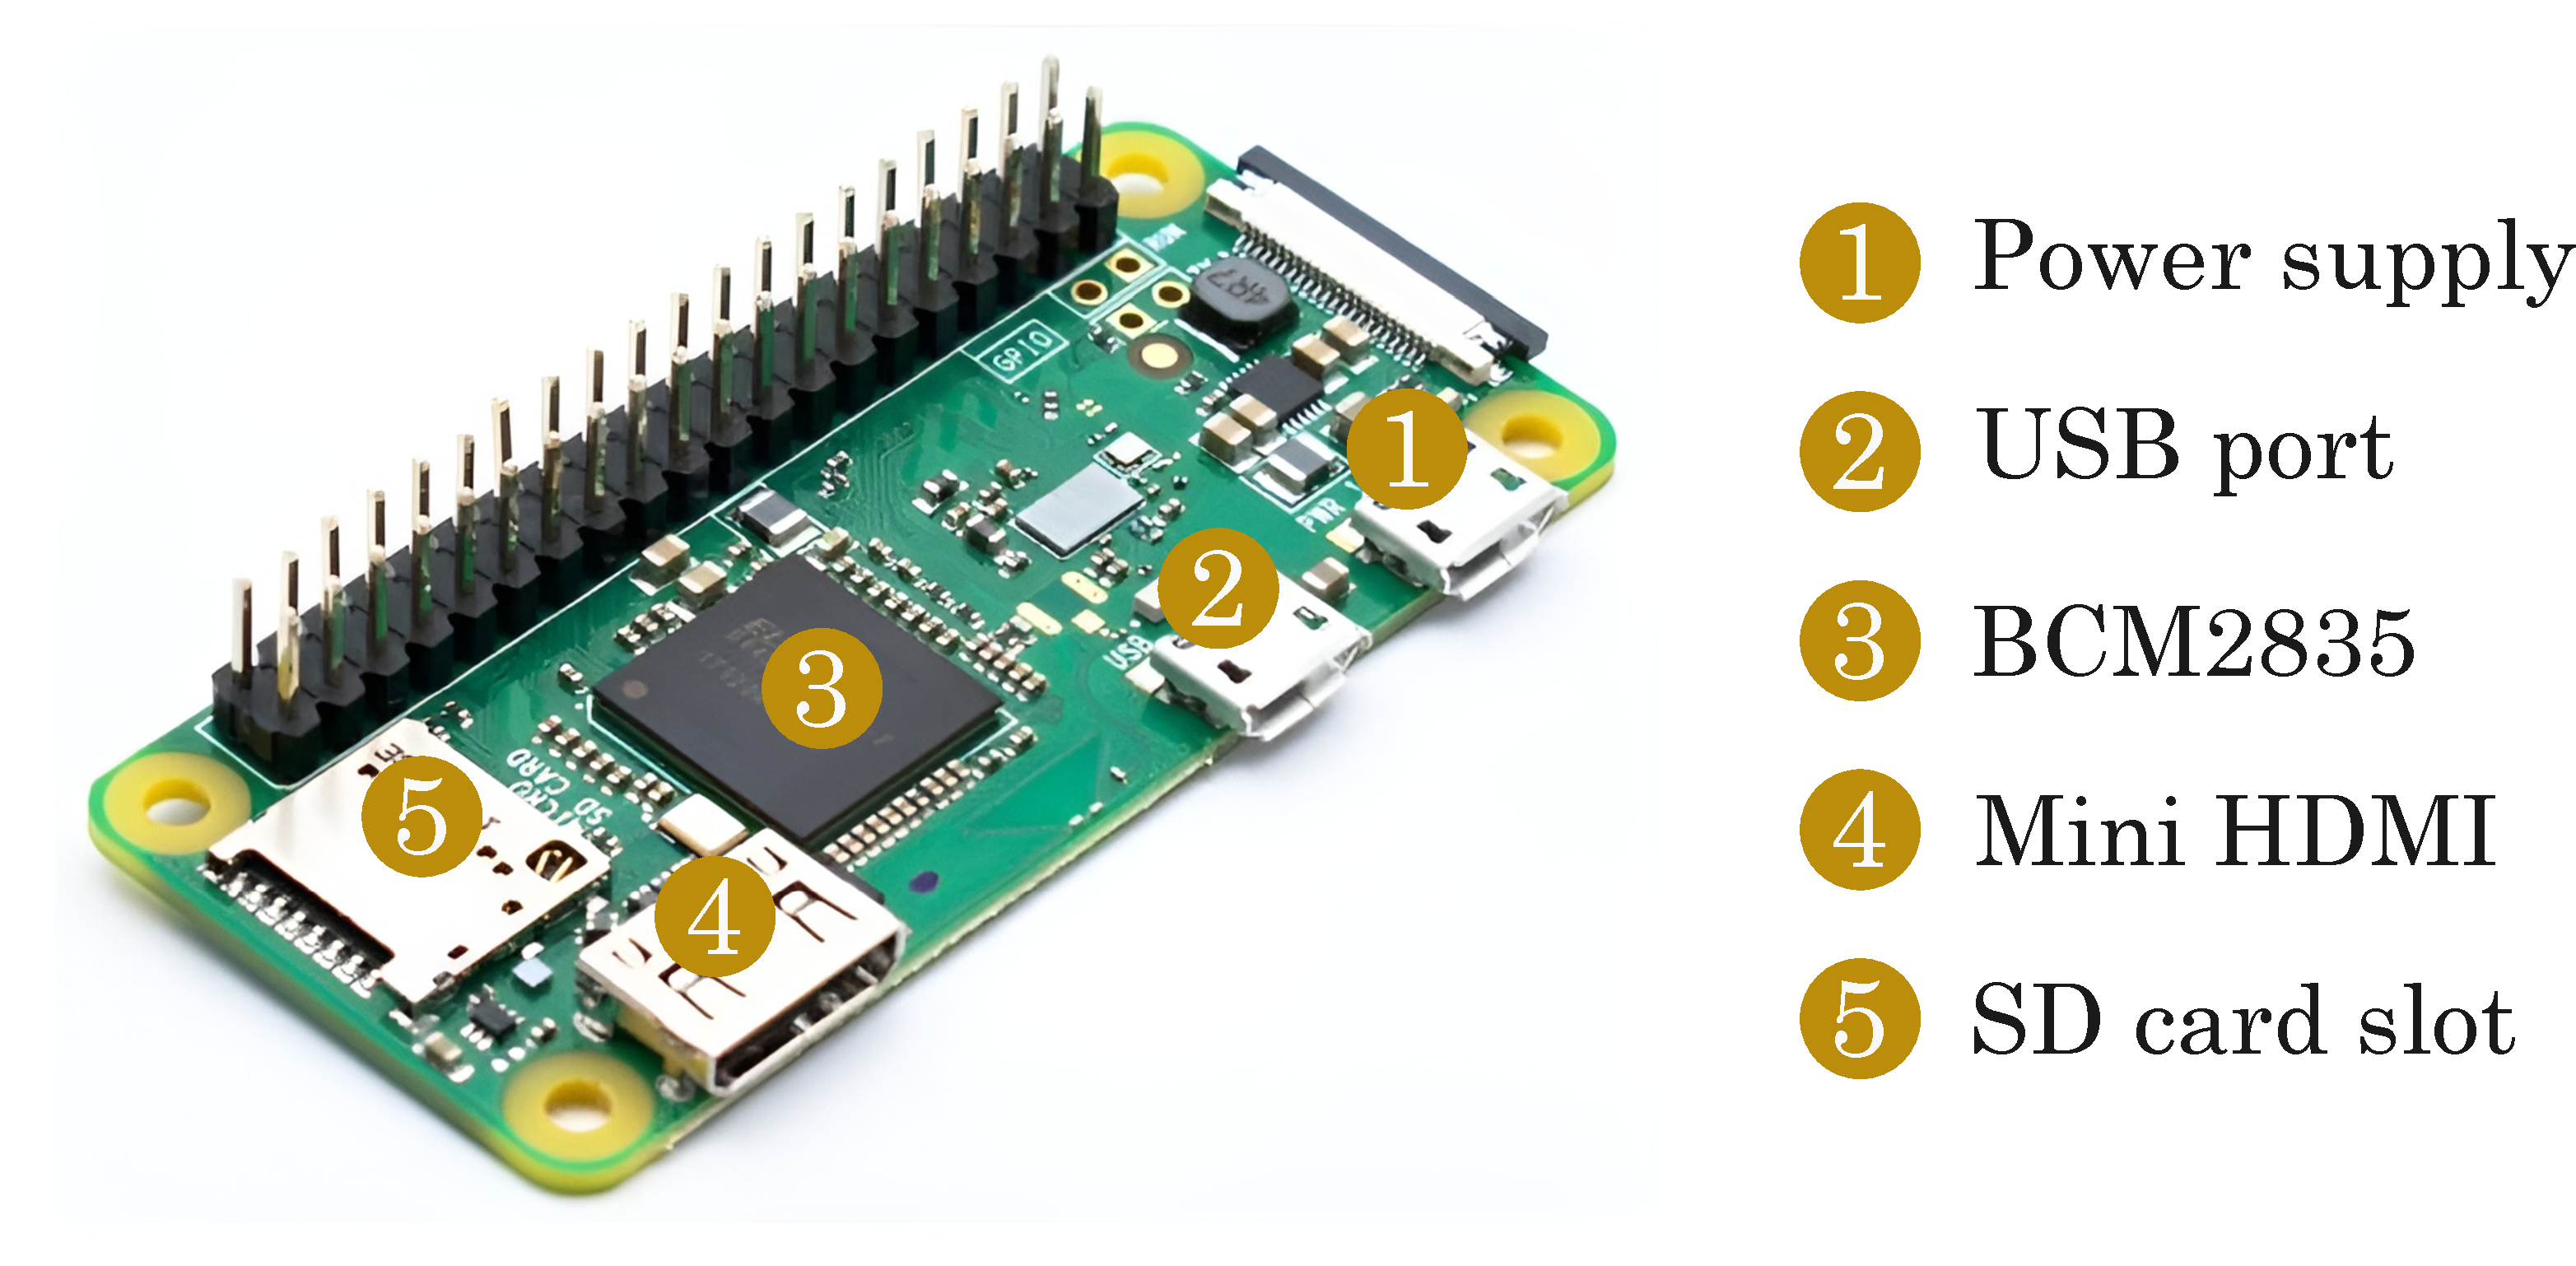
\includegraphics[width=0.65\textwidth]{img/diagrams/rpi_zero.pdf}
		\caption{Raspberry Pi Zero board}
		\label{Raspberry Pi Zero board}
	\end{figure}
	
	In contrast to other Raspberry Pi boards, such as Raspberry Pi 4, the Zero model \textbf{aims to be a compact, cost-effective, and minimalist system}. Nonetheless, it effectively fulfills its role in illustrating fundamental principles shared by more sophisticated boards. This makes it particularly valuable for smaller non-computationally intensive projects or educational purposes. Consequently, it had been chosen as an example for implementing an ARM emulator.
	
	\section{\texttt{ARM1176JZF\_S}}
	
	\texttt{ARM1176JZF\_S} is a \textbf{single-core 800 \texttt{MHz} processor that implements the ARM11 ARM architecture version 6}. It supports both the \textit{ARM} and \textit{Thumb} instruction sets, incorporates Jazelle technology for the direct execution of \texttt{Java} \texttt{bytecodes}, and includes a set of \texttt{SIMD} instructions designed to operate on \texttt{16-bit} or \texttt{8-bit} data values within \texttt{32-bit} registers. Table \ref{Breakdown of the processor's name} provides a breakdown of the individual letters and numbers found in the processor's name.
	
	\begin{center}
		\begin{longtable}{p{.10\textwidth}p{0.8\textwidth}}
			\caption{Breakdown of the processor's name (\texttt{ARM1176JZF\_S})}
			\label{Breakdown of the processor's name}\\
			\toprule[1.5pt]
			\textbf{Section} & \textbf{Meaning}\\
			\midrule
			\endfirsthead
			\multicolumn{2}{c}{\tablename{}~\thetable{} \textit{(continued from the previous page)}}\\
			\midrule
			\textbf{Section} & \textbf{Meaning}\\
			\midrule
			\endhead
			\midrule
			\multicolumn{2}{r}{\textit{(table continues on the next page)}}\\
			\endfoot
			\bottomrule[1.5pt]
			\endlastfoot
			%
			ARM11 & Indicates that the processor belongs to the ARM11 family \\
			76 & Model identifier within the ARM11 family \\
			\texttt{J} & Presence of Jazelle technology (excution of \texttt{Java} \texttt{bytecodes}) \\
			\texttt{Z} & Support for \textit{Thumb-2} technology (mix of \texttt{16/32-bit} instructions)\\
			\texttt{F} & Support for floating-point operations \\
			\texttt{S} & \say{Secure} - presence of security features (e.g. TrustZone)\\
		\end{longtable}
	\end{center}
	
	While the majority of its functionality aligns with the principles described in previous Chapter \ref{chapter-ARM Architecture}, for a more in-depth understanding, the reader can refer to the reference manual \cite{ARM1176JZF-S}.  
	
	\section{Microcontroller \texttt{BCM2835}}
	
	\texttt{BCM2835}, a microcontroller made by the Broadcom company, \textbf{incorporates a range of memory-mapped peripherals that are made accessible to the ARM processor}. These peripherals include timers, an interrupt controller, General-Purpose Input-Output pins (\texttt{GPIO}), a Universal Serial Bus interface (\texttt{USB}), a Direct Memory Access controller (\texttt{DMA}), an \texttt{I\textsuperscript{2}C} interface, a Serial Peripheral Interface (\texttt{SPI}), and the Universal Asynchronous Receiver-Transmitter, also known as the \texttt{UART} interface \footnote{The \texttt{BCM2835} microcontroller also includes a couple of peripherals intended for use by the \texttt{GPU}. However, due to complexity reasons, they were not taken into consideration in this paper.}.
	
	All peripherals, along with their memory-mapped registers, can be found detailed in the \texttt{BCM2835} ARM Peripherals datasheet \cite{BCM2835}. 
	
	\begin{important}
		However, it has been observed to contain a number of misleading pieces of information, primarily related to typing errors. Consequently, a separate document has been generated, explicitly enumerating known errors found across various chapters \cite{BCM2835_datasheet_errata}.
	\end{important}
	
	\newpage
	
	\subsection{Memory-mapped peripherals}
	
	From the programmer's perspective, memory-mapped peripherals are \textbf{devices that can be found located on a predefined known addresses in memory} \footnote{In this context, the term \say{memory} refers to the entire address space rather than the physical memory.}. For instance, according to the datasheet, the \texttt{GPIO} controller can be found located at \texttt{0x20200000}. This concept is present in one form or another in most modern \texttt{CPU}s.
	
	In addition to the ARM's Memory Management Unit, or \texttt{MMU}, the \texttt{BCM2835} microcontroller is equipped with a second coarse-grained \texttt{MMU} responsible for mapping ARM physical addresses to system bus addresses.
	
	\begin{figure}[ht]
		\centering
		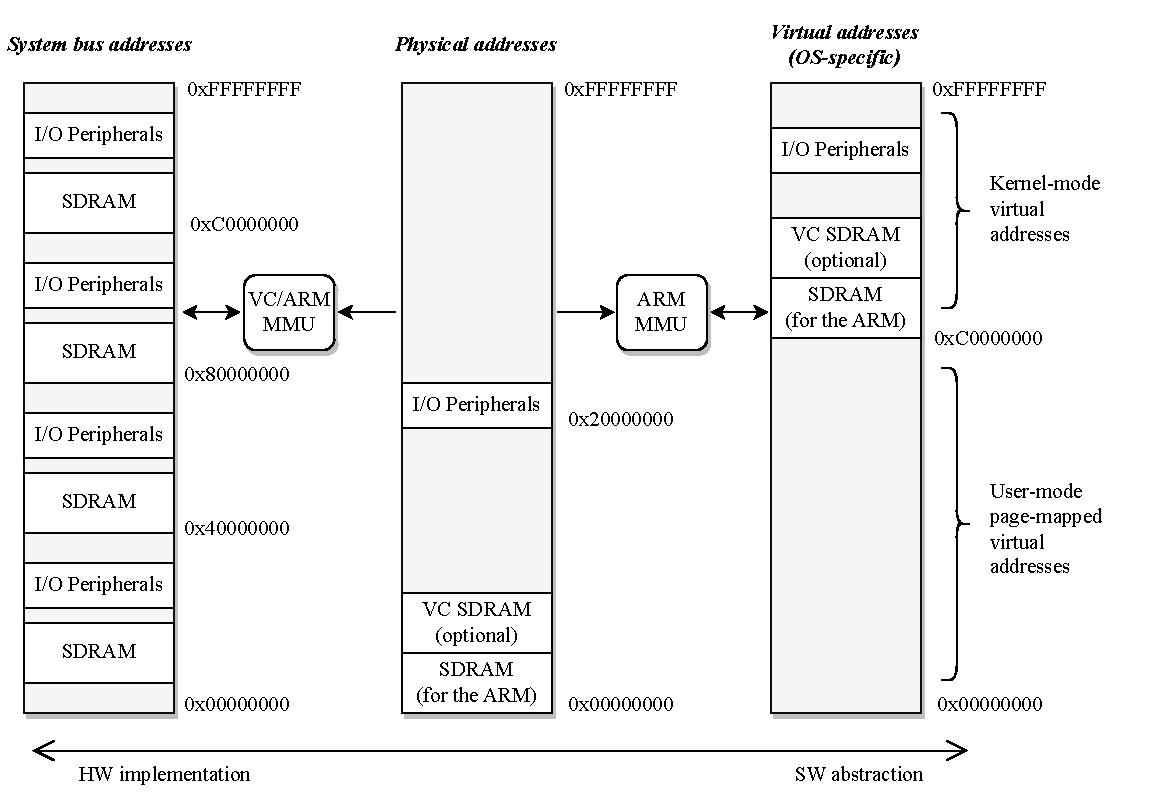
\includegraphics[width=1.0\textwidth]{img/diagrams/mmio.pdf}
		\caption{\texttt{BCM2835} address translation processes\protect\footnotemark}
		\label{BCM2835 address translation processes}
	\end{figure}
	
	\footnotetext{As an example, Figure \ref{BCM2835 address translation processes} illustrates the virtual address space utilized in \texttt{GNU/Linux}.}
	
	As shown in Figure \ref{BCM2835 address translation processes}, if the ARM \texttt{MMU} is employed, the first stage in a memory read-write operation involves translating the virtual address to a physical address based on the page table hierarchy set up by the kernel. Subsequently, once a physical address is obtained, it is mapped to a bus address that corresponds to the particular chip involved in the operation. This mapping occurs due to the fact that memory, such as flash or Synchronous Dynamic Random Access Memory, or \texttt{SDRAM}, may often be  composed of multiple chips, each potentially implementing different caching policies.
	
	\chapter{Raspberry Pi Zero Emulation}
	
	Emulating Raspberry Pi Zero on a different platform, such as x86, can offer several benefits and serve various purposes.
	
	For instance, as noted previously, it can be a powerful \textbf{tool for educational purposes}, allowing students and beginners to learn about the ARM architecture in a visual and user-friendly way. Furthermore, it can be valuable for illustrating concepts like operating system principles and embedded system development \footnote{If modularized, it can also be extended by other external modules, allowing the user to create a fully-customized system.}. The author suggests that \textbf{it could find applications in a continuous-integration development process}, where it might be utilized for executing an initial set of unit and regression tests to identify early bugs before carrying out testing on real hardware, which may not always be readily available. Examples of applicable domains may include medical devices, automotive, and other safety-related systems. Another potential benefit is that it implicitly provides a level of isolation, which \textbf{allows developers to experiment with potentially risky code} without worrying about damaging their board.
	
	All these reasons are further accentuated by ARM's omnipresence, as it is arguably one of the most widely adopted architectures worldwide.
	
	\newpage
	
	\section{Terminology}
	
	The following terms are sometimes used interchangeably. However, they fundamentally differ in the purposes they serve. Therefore, it is essential to explain them in order to establish a common understanding of their respective roles.
	
	\subsection{Simulation}
	
	In general, a simulation is a computer program designed to replicate a specific process or sequence of events, with the goal of gaining a thorough understanding of its behavior, especially in cases where a comprehensive analytical mathematical solution may be unknown. Simulations are typically parameterized, allowing them to be re-run with different input parameters to investigate how different changes in these parameters impact the observed values. They are commonly employed in various scenarios, such as modeling traffic in a city, simulating disease outbreaks, or predicting weather conditions \cite{computer-simulations}.
	
	\subsection{Emulation} \label{subsection-Emulation}
	
	In emulation, each instruction of architecture \textit{A}, an emulated architecture, is replaced with one or more instructions of architecture \textit{B}, the underlying architecture \cite{computer-emulation}. This typically results in an implicit slowdown in performance as it requires more operations to achieve the same functionality. The primary advantage of an emulator is that it enables the execution of a program that is not originally written for the underlying architecture. Some popular examples of emulators include \break DOSBox \cite{DOSBox}, which can be used for playing retro video games on a modern computer, and QEMU \cite{QEMU}, a full-emulation system capable of running various architectures.
	
	\subsection{Virtualization}
	
	Unlike emulation, virtualization allows the execution of a guest application, possibly written for a different operating system, directly on the underlying hardware \cite{computer-virtualization}. As shown in Figure \ref{Emulation vs. virtualization}, this is achieved through a \textit{hypervisor}, installed on top of the host operating system, which manages the execution of multiple distinct host machines that remain \say{invisible} to each other. Examples of such hypervisors include Xen, KVM, and Microsoft's Hyper-V. These days, virtualization plays a vital role in cloud-based solutions, as it enables dynamic allocation of virtual machines that can be utilized for various purposes, such as web servers, load balancers, computing units, and more. There are also other types of virtualization techniques, such as \textit{paravirtualization} or \textit{full virtualization}. In the case of further interest in this topic, the reader is encouraged to seek other sources of information, such as the \textit{Hardware and Software Support for Virtualization} book authored by Edouard Bugnion, \break et al. \cite{computer-virtualization-other}.
	
	Another popular technology that belongs to the emulation/virtualization category is Docker. However, it adopts a slightly different approach by primarily emulating software rather than the underlying hardware.
	
	\begin{figure}[ht]
		\centering
		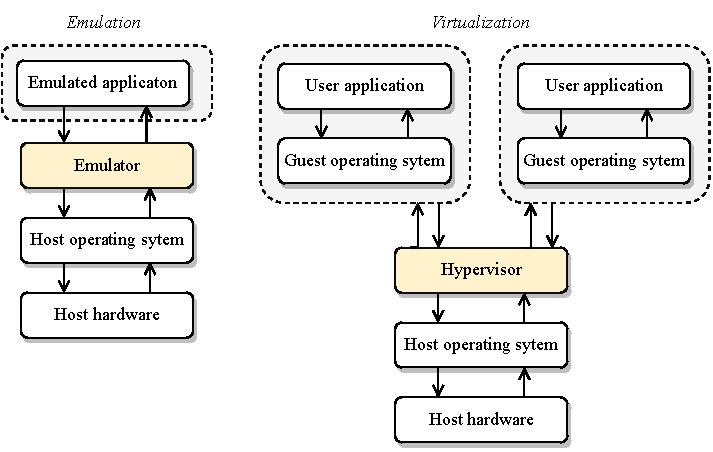
\includegraphics[width=0.85\textwidth]{img/diagrams/emulation_vs_virtualization.pdf}
		\caption{Emulation vs. virtualization}
		\label{Emulation vs. virtualization}
	\end{figure}
	
	\section{Existing Solutions}
	
	There are several available solutions that can serve as ARM emulators. However, it becomes evident that not all of them may be entirely suitable for the comprehensive and configurable emulation of an embedded environment. The following sections provide a review of some existing ARM emulators.
	
	\subsection{CPUlator}
	
	CPUlator is a sophisticated online emulator and debugger that offers \textbf{support not only for ARMv7 but also for MIPS and Nios II architectures} \cite{CPUlator}. It is specifically designed as a tool for learning assembly-language programming and gaining insight into computer organization. As a \textbf{web browser-based application}, it can be accessed from any device, making it an \textbf{excellent starting point for beginners}, as it does not require any installation. This accessibility is particularly advantageous for those who might be deterred by the complexities of installing a custom build of QEMU, for example.
	
	\begin{figure}[ht]
		\centering
		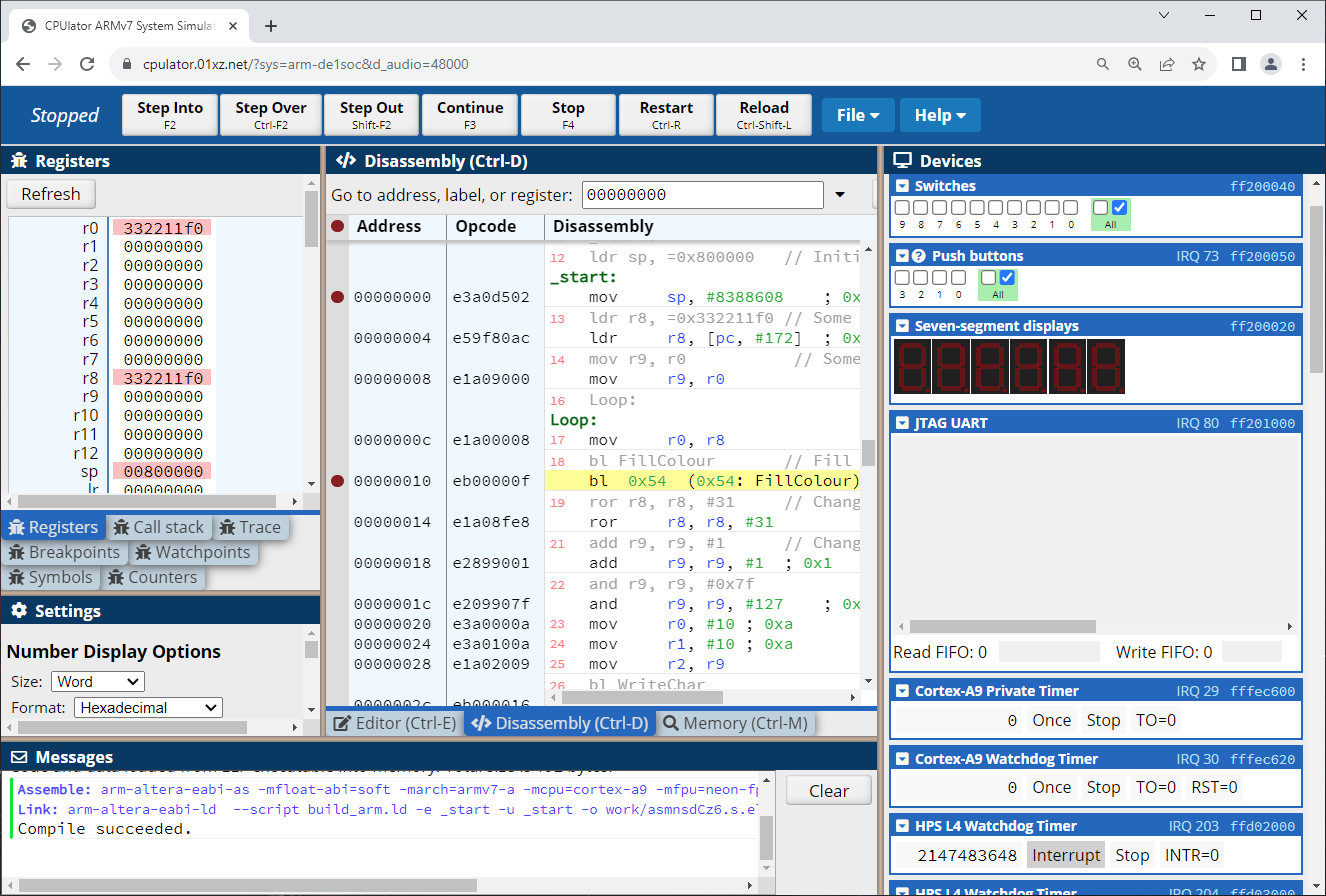
\includegraphics[width=0.9\textwidth]{img/diagrams/cpulator.png}
		\caption{CPUlator}
		\label{CPUlator}
	\end{figure}
	
	\newpage
	
	Its core is written in \texttt{C++} and compiled into WebAssembly, resulting in a user-friendly modern-looking interface that offers various debugging features such as breakpoints, single step, reverse step, step over function, step out of a function, modifying registers, showing the stack call, and more. The overall user interface can be seen in Figure \ref{CPUlator}. An input file \footnote{It supports both the \texttt{C} programming language and \texttt{ARMv7} assembly.} can either be loaded from the user's computer or entirely written and compiled using its built-in editor. In addition to the built-in compiler, it allows the user to directly upload an already built binary file. 
	
	According to its documentation, CPUlator boasts an outstanding emulation speed of 13 mega-instructions per second. As far as ARM is concerned, it features a 4 \texttt{GB} flat memory model with a maximum usable memory of 2042 \texttt{MB}. It also incorporates several input/output devices including a Video Graphics Array, or \texttt{VGA}, buttons, watchdog timers, seven-segment displays, and more. However, the integration of custom external peripherals would be a welcomed feature.
	
	Despite its support for floating-point numbers, CPUlator \textbf{lacks support for a memory-management unit}, making it impossible to leverage the full 4 \texttt{GB} address space. Similarly, it \textbf{restricts the user from switching the default \texttt{CPU} mode}, rendering it unsuitable for demonstrating most of the operating system principles. Nevertheless, it successfully fulfills its intended purpose as an excellent tool for learning the ARM assembly language.
	
	\subsection{ARMSim\#}
	
	Another tool designed primarily for educational purposes is the ARMSim\# emulator, developed at the University of Victoria in Canada \cite{ARMSim}. This \textbf{desktop application, created using the \texttt{.NET} technology}, allows users to observe and debug the execution of ARM assembly programs on a system utilizing the ARM7TDMI \break processor \footnote{As mentioned previously in Chapter \ref{chapter-ARM Architecture}, this processor was widely adopted by the cell phone industry. However, it is no longer licensed by ARM and may be considered outdated.}, which implements the \textbf{ARMv4 architecture}. The user interface can be seen in Figure \ref{ARMSim}. Similar to CPUlator, it supports debugging features such as stepping through the source code and viewing the current contents of both the \texttt{CPU} registers and memory. According to the CPUlator's comparison chart, ARMSim\# is claimed to be capable of executing up to 3 mega-instructions per second \cite{CPUlator}.
	
	\begin{figure}[ht]
		\centering
		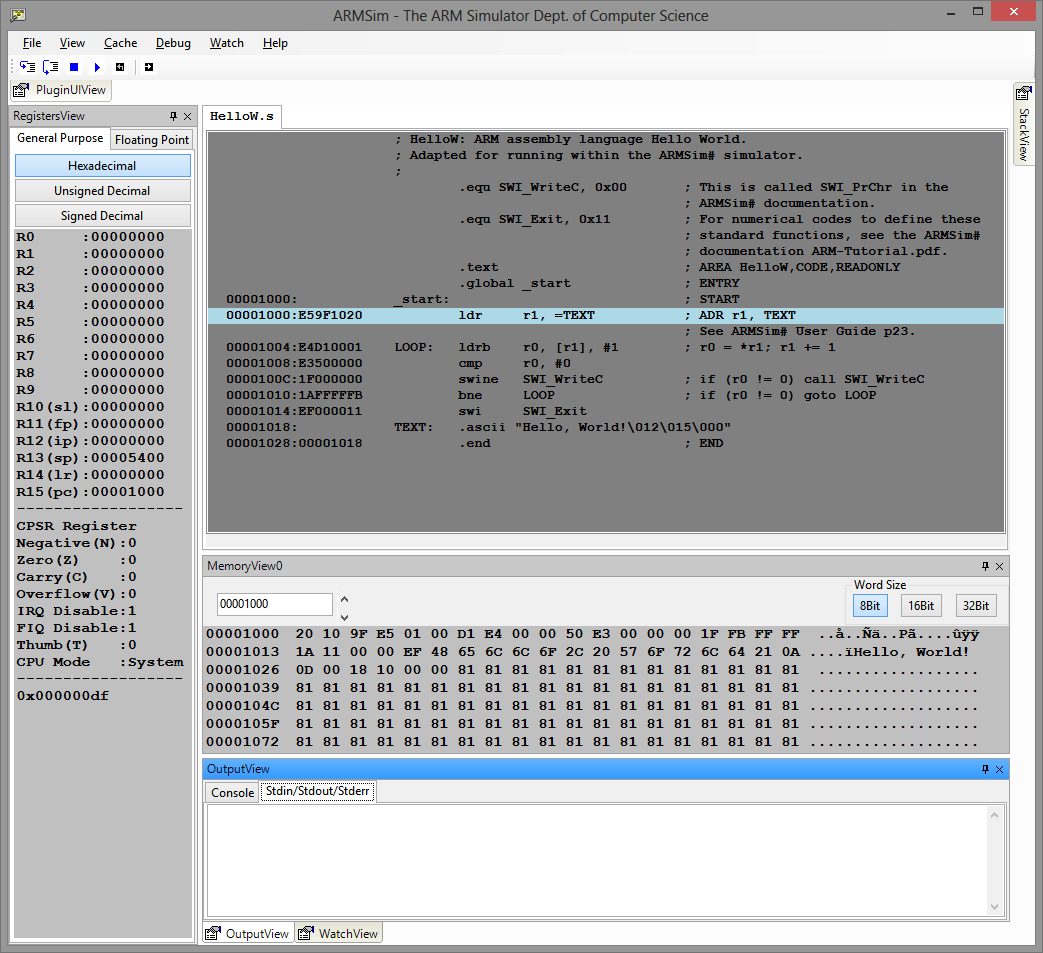
\includegraphics[width=0.9\textwidth]{img/diagrams/armsim.png}
		\caption{ARMSim\#}
		\label{ARMSim}
	\end{figure}
	
	The emulator \textbf{features so-called plugins that further extend its functionality in a modular fashion}. Examples of these plugins may include \textit{SWIInstructions}, which encapsulates a variety of system calls, such as reading and writing to a file, or \textit{EmbestBoard}, which allows the core to interact with external peripherals such as a keyboard, segment display, or a 40x15 display — all of which are also interacted with via system calls.
	
	ARMSim\# also supports vector floating-point instructions; however, similar to CPUlator, it \textbf{lacks support for a memory-management unit}. It can be concluded that while it finds application in learning the ARM assembly language, it does not provide features for advanced system-level programming, like developing an operating system, \textbf{nor does it support the concept of memory-mapped peripherals}, which can be found in the majority of modern embedded devices.
	
	\subsection{QEMU}
	
	QEMU stands out as a powerful \textbf{cross-platform full-emulation system}, written in \texttt{C}, with the capability to emulate operating systems across various architectures, including x86, MIPS, ARM, and PowerPC \cite{QEMU}. While it may not offer the same visual appeal as the previous examples, its versatility surpasses them. QEMU can operate in both graphics mode, if supported by the guest operating system, and terminal-only mode. In terms of debugging, \textbf{it allows the attachment of the \texttt{GNU} debugger}, a tool heavily utilized in Linux-based operating systems.
	
	However, when attempting to emulate the Raspberry Pi Zero environment, \textbf{QEMU does not provide a plug-and-play solution upon installation}. By default, it expects an ARM-based system to boot up from address \texttt{0x00010000}. In contrast, the Raspberry Pi Zero's \textit{first stage bootloader} necessitates the kernel's reset vector to be situated at address \texttt{0x00008000}.
	
	Consequently, users face two options. They can either relocate their kernel to the required address or modify QEMU's source code to change the kernel load address and create a custom build. It is important to mention that the second approach may pose certain challenges for beginners. Conveniently, the entire process of running a custom image built for Raspberry Pi Zero is detailed in the KIV/OS - dodatek A document \cite{KIV-OS-dotatek-A}.
	
	While QEMU does support most of the features that the previous emulators lack, its versatility may also come with certain disadvantages when emulating the Raspberry Pi Zero environment. Specifically, there are reported \textbf{issues related to the system timer}, hindering the implementation of a preemptive scheduler in the custom operating system. Furthermore, it lacks a straightforward solution for attaching external hardware peripherals. In the case of Raspberry Pi, it can be inferred that QEMU might not be the optimal choice for emulating such an embedded environment, given its primary focus on emulating more general-purpose operating systems.
	
	\section{General Requirements} \label{General Requirements}
	
	Reviewing existing solutions renders a set of general requirements for an ideal emulator designed to emulate the Raspberry Pi Zero environment.
	
	\paragraph{Preciseness}
	
	It is evident that the emulator should identically mimic a real Raspberry Pi Zero board. This is arguably the most crucial requirement to fulfill, as failing to do so could result in  unexpected behavior. Ideally, if the user compiles and runs their application inside the emulator, they should be presented the with same output as if it was executing on real hardware. However, this may sometimes be challenging to achieve, especially considering time constraints mentioned previously in \break Section \ref{subsection-Emulation}.
	
	\paragraph{Effectiveness}
	
	In terms of performance, a slowdown in emulation speed is nearly inevitable. Nevertheless, the emulator should leverage modern technologies to mitigate these effects. Consequently, the use of certain programming languages like Python might be ruled out, as they could adversely impact overall performance, which is discussed further in Section \ref{Programming Language}. Moreover, the emulator should strive to consume only a reasonable amount of the system's resources.
	
	\paragraph{User-friendliness}
	
	The final emulator should introduce users to embedded development principles through a visual and user-friendly interface \footnote{In practice, this can be measured, for instance, through surveys.}. They should have the capability to perform all the previously mentioned actions, such as setting breakpoints and viewing the contents memory and registers, without the necessity of connecting an external debugger. This is particularly crucial for beginners, as they should have access to these features effortlessly upon installation. Another essential requirement is that users should not be restricted to the use of the emulator on a single platform, such as Windows.
	
	\paragraph{Extensibility}
	
	In the embedded world, microcontrollers are frequently programmed to communicate with external devices, including motors, displays, sensors, or even other microcontrollers. Therefore, the emulator should facilitate the integration of external devices that can be developed independently of the emulator itself, thereby enabling other developers to contribute to the project. This functionality would empower users to configure a real-world scenario tailored to their specific application.
	
	%------------------------------------------------------------
	% ------ 2nd part
	%------------------------------------------------------------
	
	\chapter{Design of a Raspberry Pi Zero Emulator} \label{Design of a Raspberry Pi Zero Emulator}
	When designing a complex software system, it is important to take into consideration deciding factors such as the intended usage environment, interaction methods, system dependencies, preferred technologies, or different components constructing the final application. Addressing these questions early on enhances the likelihood of its successful completion as well as its long-term maintainability.
	
	This chapter outlines the key design decisions made within the implementation process of the \textbf{ZeroMate emulator}, which is the chosen name for the project \footnote{It combines the word \emph{Zero}, as in Raspberry Pi Zero, and \emph{Mate}, which in this case is used as a synonym for a friend or \say{buddy}.}.
	
	\section{Input} \label{Input}
	
	The emulator necessitates a single input file in the \texttt{ELF} format, simplifying the Raspberry Pi's booting process. In this process, the \textit{stage 1 bootloader}, residing in \texttt{ROM}, reads the contents of the \texttt{SD} card and then initiates and delegates control to the \texttt{GPU}, which subsequently resets the \texttt{CPU} and loads the kernel into \texttt{RAM}.
	
	This file is further referred to as the \textbf{kernel} since the emulator was designed within the context of operating systems development. Nevertheless, the input file can fundamentally represent any application intended for execution on Raspberry Pi Zero. Figure \ref{building ELF} illustrates the general process of building an \texttt{ELF} file, which contains all essential data and information required for code emulation.
	
	\subsection{Executable and Linkage Format}
	
	\texttt{ELF} stands for \emph{Executable and Linkage Format} \cite{ELF}, and it is one of the most commonly used formats for executable files, especially on Unix-like systems. There are a number of other representations used in embedded development. For instance, the \emph{Motorola S-Record format}, or \texttt{SREC} for short, is often used for programming non-volatile types of memory, such as flash or \texttt{EEPROM}. The structure of an \texttt{SREC} record is visualized in Figure \ref{srec}.
	
	In terms of this project, the key advantage of \texttt{ELF} over \texttt{SREC} is that \texttt{ELF} is \textbf{used for both linkage and execution}. Therefore, if the kernel is compiled with debug symbols turned on, the symbol table stored in the final \texttt{ELF} file can be used during the parsing process, which is discussed in Section \ref{ELF Loader}, to provide the user with function names as they were used in the source code, which should improve the readability of the final disassembly. \texttt{SREC}, on the other hand, is \textbf{only used for execution}. Therefore, it can be viewed as highly compressed as it comprises only the necessary information for uploading firmware onto a microcontroller, which is commonly referred to as flashing. 
	
	It can be concluded that \texttt{ELF} provides more information that can be useful when reconstructing the original source code. Hence, it is used as the supported format for the input files. It is worth mentioning that this choice does not have as much impact on the core functionality as it does on visual aspects, which is discussed more in detail in Section \ref{User Interface}.
	
	\begin{figure}[ht]
		\centering
		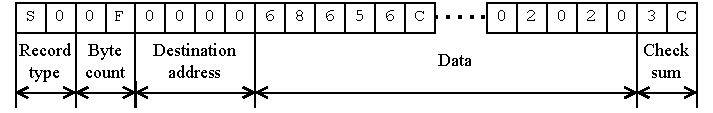
\includegraphics[width=.95\textwidth]{img/diagrams/srec.pdf}
		\caption{Single \texttt{SREC} record (16-bit addressing)}
		\label{srec}
	\end{figure}
	
	\begin{figure}[ht]
		\centering
		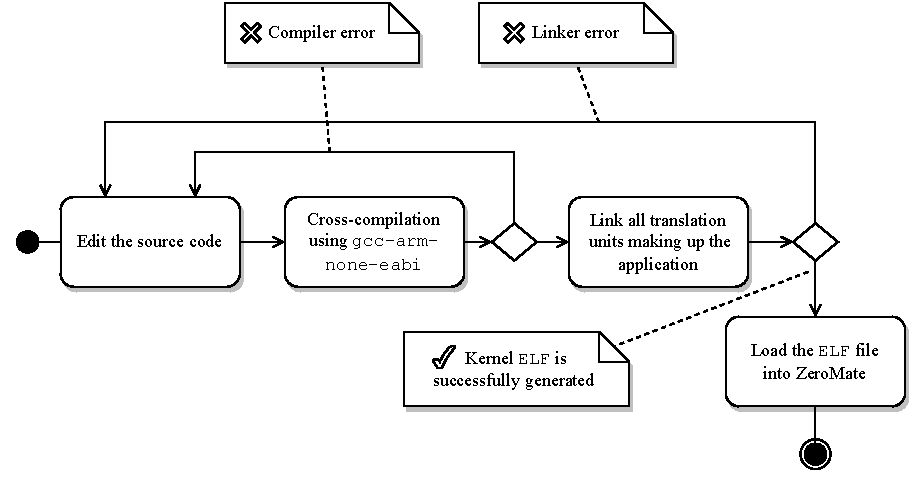
\includegraphics[width=1.0\textwidth]{img/diagrams/kernel_build_activity_diagram.pdf}
		\caption{Process of building an \texttt{ELF} file (input for the emulator)\protect\footnotemark}
		\label{building ELF}
	\end{figure}
	
	\footnotetext{Cross-compiling is a process where the source code targets a different platform than the one it is compiled on.}
	
	\newpage
	
	\section{User's Interaction}
	
	As shown in the deployment diagram in Figure \ref{Deployment diagram of the ZeroMate emulator}, the emulator was \textbf{designed to run as a native desktop application on Windows, Linux, and MacOS operating systems}. It places a strong emphasis on visualization, serving as a debugging tool to assist with troubleshooting embedded applications targeting Raspberry Pi Zero.
	
	The primary interaction with the system, from the user's perspective, is visualized in Figure \ref{Primary use-cases of the ZeroMate emulator}, where the user is provided with an interface that allows them to load an input file as well as to control the state of the emulation.
	
	\begin{figure}[ht]
		\centering
		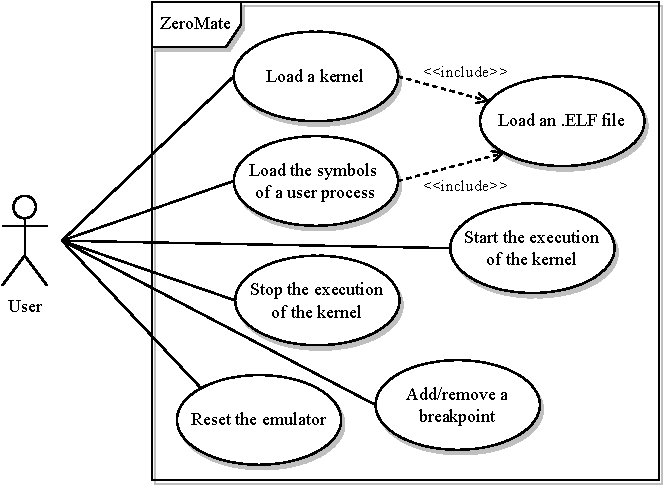
\includegraphics[width=.8\textwidth]{img/diagrams/use_case_diagram.pdf}
		\caption{Primary use-cases of the ZeroMate emulator}
		\label{Primary use-cases of the ZeroMate emulator}
	\end{figure}
	
	\begin{figure}[ht]
		\centering
		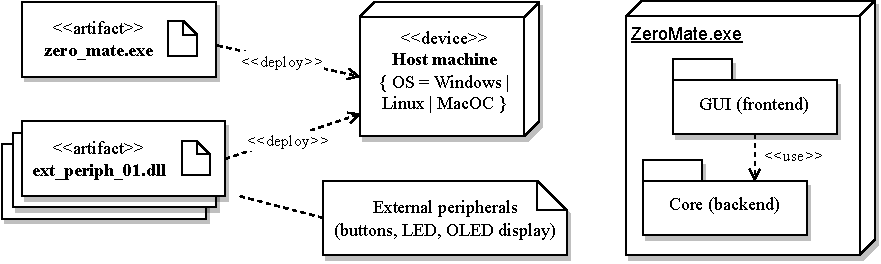
\includegraphics[width=1.0\textwidth]{img/diagrams/deployment_diagram.pdf}
		\caption{Deployment diagram of the ZeroMate emulator}
		\label{Deployment diagram of the ZeroMate emulator}
	\end{figure}
	
	\newpage
	
	The main application is designed as a \textbf{two-tier architecture}. In this arrangement, the top layer, which is the \texttt{GUI}, serves the dual purpose of visualizing data and acting as the primary user interface. The following chapters delve into the architectural structure of the core part of the emulator.
	
	\section{Core Components}
	
	There are a number of different components working alongside to achieve a thorough emulation of a given kernel. Among these components, the \texttt{ARM1176JZF\_S} component, which represents the \texttt{CPU} itself, may arguably stand out as the most complex one due to its encapsulation of various sub-components, including the \texttt{CPU} context, \texttt{ALU}, \texttt{MMU}, \texttt{ISA} decoder, and more. The role of every component will be examined further in the following sections.
	
	\begin{figure}[ht]
		\centering
		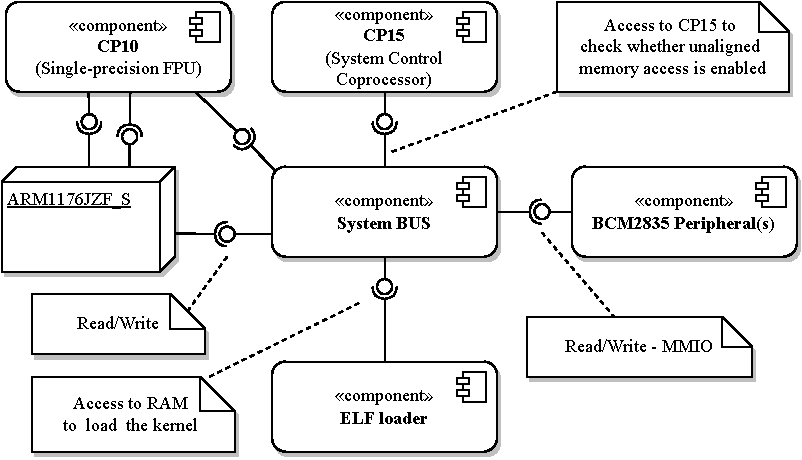
\includegraphics[width=1.0\textwidth]{img/diagrams/core_component_diagram.pdf}
		\caption{Core components of the ZeroMate emulator}
		\label{Components of the core of the ZeroMate emulator}
	\end{figure}
	
	Figure \ref{Components of the core of the ZeroMate emulator} illustrates the fundamental interactions among the core components. It can be observed that the majority of the components communicate with one another via the system bus \footnote{What ZeroMate denotes as the system bus is typically regarded as the primary \texttt{CPU} bus.}. For example, when the \texttt{CPU} executes a load/store instruction, it propagates the target address to the system bus, and the system bus then forwards the request to the corresponding peripheral associated with that address.
	
	\newpage
	
	\subsection{System Bus} \label{System Bus}
	
	As mentioned previously, the system bus serves as an \textbf{intermediate unified interface} for accessing the \texttt{RAM} or any of the \texttt{BCM2835} memory-mapped peripherals \cite{BCM2835}. The primary functions this interface provides can be seen in Listing \ref{System bus interface for I/O operations}. Each peripheral that is meant to be mapped into the address space must implement the same interface, so the bus can forward the read/write request independently of the peripheral's implementation (see Section \ref{Peripherals}). All actions associated with the request itself are then handled internally within the target peripheral.
	
	\begin{figure}[ht]
		\centering
		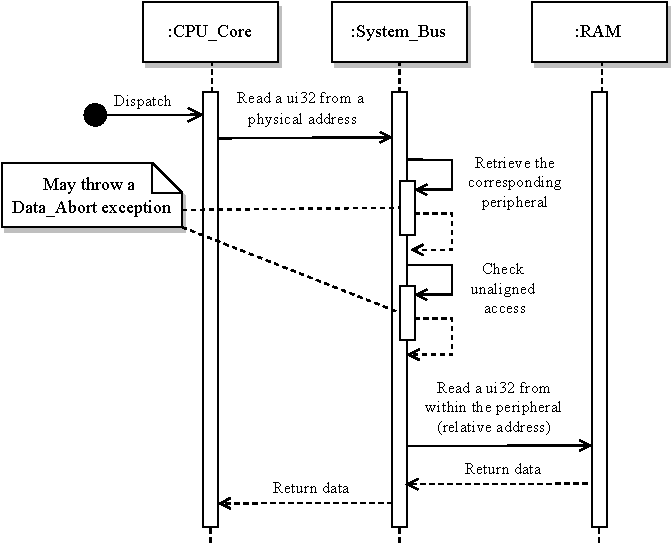
\includegraphics[width=.9\textwidth]{img/diagrams/bus_sequence_diagram.pdf}
		\caption{Example of a read/write data request issued by the \texttt{CPU}}
		\label{Example of a read/write data request issued by the CPU}
	\end{figure}
	
	As shown in Figure \ref{Example of a read/write data request issued by the CPU}, there are two internal steps the system bus carries out before proceeding with the request. First, it needs to determine what peripheral should the request be forwarded to. Secondly, it checks whether unaligned memory access is taking place or not.
	
	\begin{important}
		In reality, the main system bus does not manage peripherals the same way it does in ZeroMate. It only serves as a medium for connecting different types of memory-mapped devices. Nevertheless, from an architectural point of view, it is a reasonable place for implementing common validity checks as it plays the role of a single point of access to all memory-mapped peripherals.
	\end{important}
	
	\newpage
	
	Additionally, the system bus ensures that the peripheral receives an \textbf{address relative to its location in the address space} \footnote{The relative address is calculated as the address contained in the \texttt{R/W} request issued by the \texttt{CPU} minus the address of the peripheral on the system bus.}. In other words, it does not have any knowledge about its location on the bus, which is desired, as it decreases coupling and increases cohesion between the two components \cite{Coplien}.  
	
\begin{code}{C++}{System bus interface for \texttt{I/O} operations \label{System bus interface for I/O operations}}
class CBus final {
	public:
		template<typename Type>
		void Write(std::uint32_t addr, Type value);
		
		template<typename Type>
		[[nodiscard]] Type Read(std::uint32_t addr);
};
\end{code}
	
	\begin{important}
		It can be argued that permitting the reading or writing of a general data type may diverge from real hardware specifications, as the system bus is typically of a fixed size, e.g. 32 bits. This simplification was made for convenience reasons when accessing predefined data structures in the \texttt{RAM}, such as the page table(s).
	\end{important}
	
	\subsubsection{Managing Peripherals} \label{Managing Peripherals}
	
	The system bus component maintains a collection of references to all memory-mapped input-output devices, further referred to as \texttt{MMIOs}. Whenever a peripheral needs to be attached to the bus, it is inserted into the appropriate position within the collection, which is visualized in Figure \ref{Collection of memory-mapped peripherals}. This ensures that the entire collection remains sorted in ascending order based on the starting addresses of the peripherals. This property enables the use of a binary search algorithm, resulting in faster lookup times, particularly in $\mathcal{O}(\log n)$ time complexity \cite{binary-search}, which is crucial for improving the overall speed of the emulation.
	
	According to statistics, on average, \textbf{load-store instructions account for more than 50\% of all instructions in an x86 application} \cite{x86}. Although this research applies to a different architecture, it is reasonable to conclude that optimizing peripheral access efficiency might be crucial for emulation speed.
	
	When connecting a peripheral, the bus must also ensure that there is no overlap between two peripherals and that they all fit within the address space, which, on a \texttt{32-bit} architecture, spans out to \texttt{4GB}.
	
	\begin{figure}[ht]
		\centering
		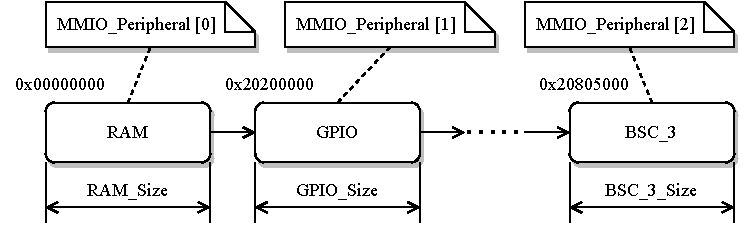
\includegraphics[width=.9\textwidth]{img/diagrams/bus_peripherals.pdf}
		\caption{Collection of memory-mapped peripherals}
		\label{Collection of memory-mapped peripherals}
	\end{figure}
	
	\subsubsection{Unaligned Memory Access}
	
	Unaligned memory access occurs when the \textbf{\texttt{CPU} attempts to read or write data from an address that is not divisible by the word size}. For example, reading 4 bytes from address \texttt{0x00000011} triggers unaligned access as the address is not \texttt{word}-aligned \footnote{A \texttt{word} is a fixed-size number of bits that the \texttt{CPU} can process as a single unit. In the case of \texttt{ARM1176JZF\_S}, one \texttt{word} equivocates to 4 bytes.}. Nevertheless, this behavior can optionally be disabled, for example, for compatibility reasons, in the \textit{System Control Co-processor} (\texttt{CP15}) using the sequence of ARM instructions shown in Listing \ref{Enabling unaligned access in CP15}.
	
\begin{code}{C++}{Enabling unaligned access in \texttt{CP15} \label{Enabling unaligned access in CP15}}
mrc p15, #0, r0, c1, c0, #0  ;@ Copy ctrl reg of CP15 to R0
orr r0,  #0x400000           ;@ Set bit 22 in R0
mcr p15, #0, r0, c1, c0, #0  ;@ Update CP15
\end{code}
	
	\newpage
	
	\subsection{Executable and Linkage Format File Loader} \label{ELF Loader}
	
	The main purpose of this module is to \textbf{parse an input \texttt{ELF}} file and copy the \texttt{.text} section, which contains source code instructions, \texttt{word} by \texttt{word}, into \texttt{RAM}, as specified by the linker script. Additionally, it performs code disassembly, which is a process of reconstructing the source code from machine code. This allows the user to observe individual instructions in a more user-friendly way as they are executed.
	
	For visualization purposes, the component also features the capability to parse an \texttt{ELF} file without copying its data into memory, which can be useful for viewing user processes that are compiled separately from the kernel itself. During this process, the \textbf{\texttt{ELF} loader also demangles all symbols} found in the input file \footnote{Demangling is a process of transforming \texttt{C/C++} \texttt{ABI} identifiers into the original \texttt{C/C++} source~\cite{demangling}.}, thereby presenting the user with function names that have not undergone modification by the compiler for its internal purposes. An example illustrating symbol demangling is demonstrated in Listing \ref{Example of symbol demangling}.
	
\begin{code}{C++}{Example of symbol demangling \label{Example of symbol demangling}}
Demangle("_ZNSt6vectorIiSaIiEE9push_backERKi") = 
"std::vector<int,std::allocator<int>>::push_back(int const&)"
\end{code}
	
	Figures \ref{Loading an input ELF file (kernel)} and \ref{Internal logic of the ELF Loader component} illustrate the steps and components involved in loading and parsing an input \texttt{ELF} file.
	
	\begin{figure}[ht]
		\centering
		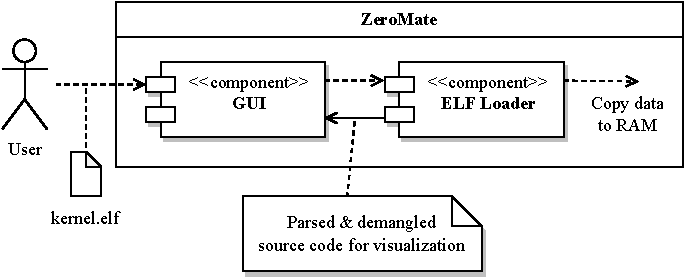
\includegraphics[width=.9\textwidth]{img/diagrams/elf_diagram_2.pdf}
		\caption{Loading an input \texttt{ELF} file (kernel)}
		\label{Loading an input ELF file (kernel)}
	\end{figure}
	
	\newpage
	
	\begin{figure}[ht]
		\centering
		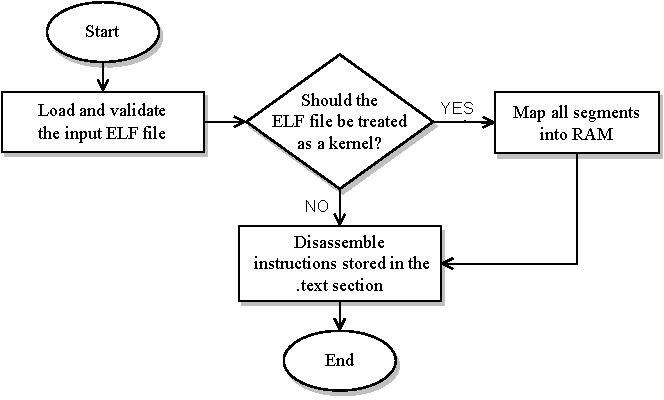
\includegraphics[width=.9\textwidth]{img/diagrams/elf_diagram.pdf}
		\caption{Internal logic of the \texttt{ELF} Loader component}
		\label{Internal logic of the ELF Loader component}
	\end{figure}
	
	It is important to emphasize that ZeroMate does not perform the tasks of parsing an \texttt{ELF} file and demangling symbols all by itself. Instead, it utilizes two external open-source libraries, \textit{ELFIO} \cite{elifio} and \textit{Demumble} \cite{demumble}, to accomplish these functions.
	
	\subsection{\texttt{BCM2835} Peripherals} \label{Peripherals}
	
	\textbf{ZeroMate distinguishes between two types of peripherals} - those directly integrated within the microcontroller, such as \texttt{RAM}, \texttt{ARM} timer, or the interrupt controller, and those referred to as external peripherals, which are externally connected to another internal peripheral, the \texttt{GPIO} pins, forming a cascading set of connected peripherals. Examples of external peripherals may include buttons, switches, \texttt{LED}s, displays, or keyboards. The following sections focus on the internal peripherals of Raspberry Pi Zero.
	
	\newpage
	
	\begin{figure}[ht]
		\centering
		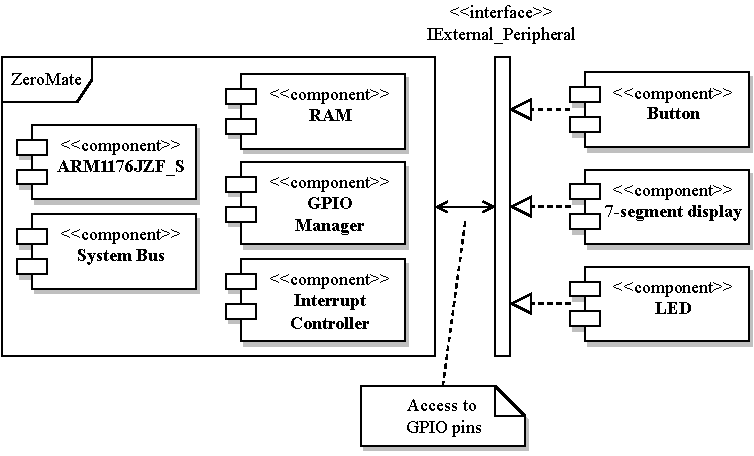
\includegraphics[width=.9\textwidth]{img/diagrams/peripherals.pdf}
		\caption{Internal vs External peripherals}
		\label{Internal vs External peripherals}
	\end{figure}
	
	In Section \ref{System Bus}, it is explained that the system bus manages a collection of references to all peripherals that are mapped into the address space. Using a general interface, the bus does not need to be concerned about how each peripheral functions internally. In a proxy-like fashion, it simply forwards a \texttt{R/W} request initiated by the \texttt{CPU} to the corresponding peripheral. 
	
	Every \texttt{BCM2835} peripheral encapsulates a set of registers, whose functions are detailed in the \texttt{BCM2835} manual \footnote{As mentioned previously, the \texttt{BCM2835} manual is known to contain several typographical errors. As a result, the community surrounding it published a list of these errors along with their respective corrections \cite{BCM2835_datasheet_errata}.} \cite{BCM2835}. By reading from or writing to these registers, the internal state of the peripheral can be modified, which is specific for each peripheral.
	
	\begin{figure}[ht]
		\centering
		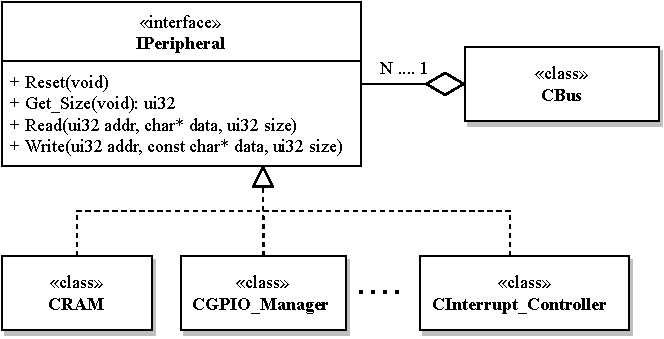
\includegraphics[width=.82\textwidth]{img/diagrams/peripheral_interface.pdf}
		\caption{Hierarchy of internal peripherals}
		\label{Hierarchy of internal peripherals}
	\end{figure}
	
	The \texttt{Get\_Size()} method shown in Figure \ref{Hierarchy of internal peripherals} is used primarily for detecting bus collisions when mapping peripherals into the address space, which was mentioned previously in Section \ref{Managing Peripherals}.
	
	\begin{figure}[ht]
		\centering
		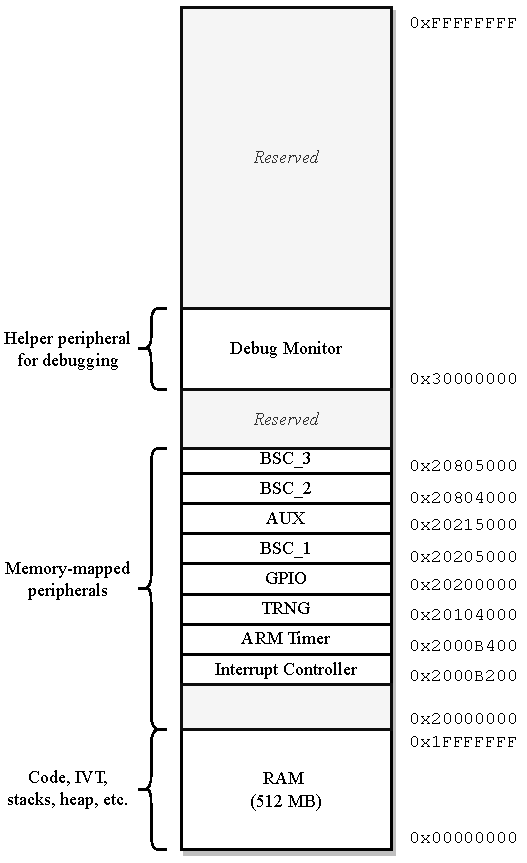
\includegraphics[width=0.72\textwidth]{img/diagrams/address_space.pdf}
		\caption{\texttt{BCM2835} physical memory layout emulated by ZeroMate}
		\label{BCM2835 memory layout emulated by ZeroMate}
	\end{figure}
	
	It can be noticed that \textbf{ZeroMate does not account for all \texttt{BCM2835} peripherals} since emulating every single one in its entirety would pose a significant complexity. Consequently, ZeroMate focuses its emulation efforts on the most frequently utilized peripherals, such as the \texttt{ARM} timer, \texttt{GPIO}, interrupt controller, and others.
	
	Nonetheless, the system's overall design is structured to allow for a smooth integration of additional peripherals in the future if needed. The following sections explain the fundamental emulation principles of each of the peripherals listed in Figure \ref{BCM2835 memory layout emulated by ZeroMate}.
	
	\subsubsection{Memory-mapped Registers} \label{Memory-mapped Registers}
	
	As mentioned previously, each \texttt{BCM2835} peripheral encapsulates a set of registers, through which the user can interact with the peripheral. From an implementation perspective, these registers can be represented as a fixed-size array of \texttt{32-bit} integers, which are addressed relative to the peripheral's base address.
	
	\begin{figure}[ht]
		\centering
		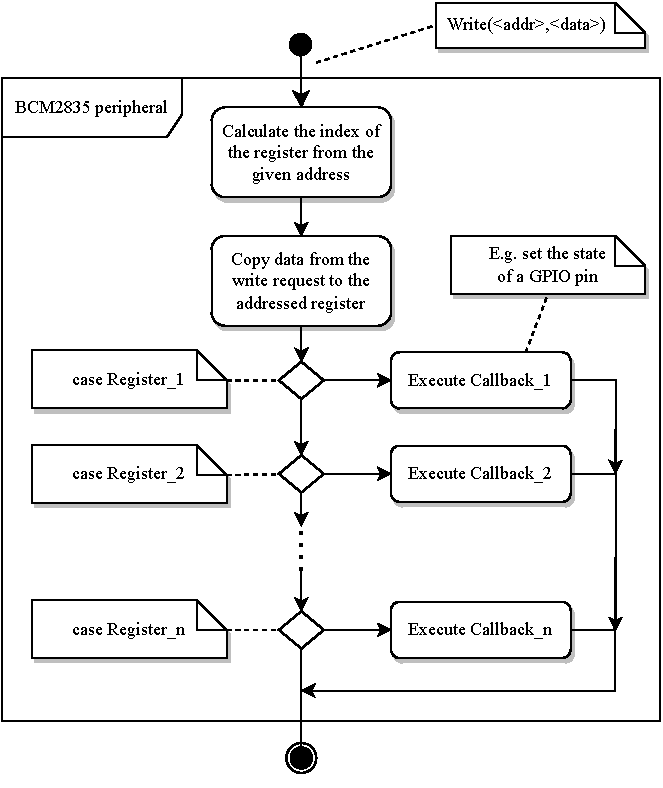
\includegraphics[width=.74\textwidth]{img/diagrams/memory_mapped_regs.pdf}
		\caption{Writing to a peripheral's register\protect\footnotemark}
		\label{Writing to a peripheral's register}
	\end{figure}
	
	\footnotetext{Reading works in a similar way. Optionally, there might be additional prior actions taken before a value is read from a peripheral's register, such as inserting a random number into the \texttt{data} register when utilizing \texttt{TRGN}, which is described in Section \ref{trng}.}
	
	Whenever a read/write request is sent through the bus, the peripheral identifies the addressed register, and the execution is then dispatched to the corresponding callback function, which carries out the necessary actions associated with that specific register. Generally, this approach, which is shown in Figure \ref{Writing to a peripheral's register}, can be applied to the vast majority of memory-mapped peripherals. 
	
	\subsubsection{System Clock Listener} \label{System Clock Listener}
	
	Optionally, each peripheral can implement the \texttt{ISystem\_Clock\_Listener} interface, which allows it to register with the \texttt{CPU} as a system clock listener. This concept is visualized in Figure \ref{ISystem_Clock_Listener interface}. Whenever an instruction is executed, the \texttt{CPU} notifies all of the system clock listeners of how many \texttt{CPU} cycles it took to execute the instruction, allowing them to update themselves accordingly. Further information on how ZeroMate emulates the execution time of individual ARM instructions can be found in Section \ref{Central Processing Unit Core}.
	
	Examples of such listeners may include the \texttt{ARM} Timer or the \texttt{AUX} and \texttt{BSC} peripherals, which encapsulate time-based hardware communication functions. These peripherals are described in Sections \ref{ARM Timer}, \ref{AUX}, and  \ref{BSC}, respectively.
	
	\begin{figure}[ht]
		\centering
		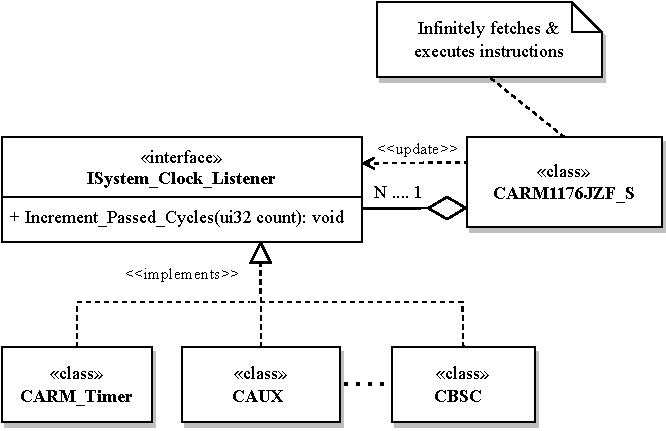
\includegraphics[width=0.86\textwidth]{img/diagrams/system_clock_listener.pdf}
		\caption{\texttt{ISystem\_Clock\_Listener} interface}
		\label{ISystem_Clock_Listener interface}
	\end{figure}
	
	It is important to mention that \textbf{updating a system clock listener is, from the emulated \texttt{CPU}'s perspective, a blocking operation}. Therefore, the peripheral's callback function should avoid any unnecessary actions that might further prevent the \texttt{CPU} from executing the next instruction. Alternatively, updating system clock listeners could be performed asynchronously within a separate thread. However, this approach would introduce additional concurrency-related challenges that would require thorough consideration.
	
	\newpage
	
	\subsubsection{Random Access Memory}
	
	From an oversimplified perspective, a computer consists of two essential components; the \texttt{CPU} and memory. One key parameter used to classify various types of memory is their ability to retain data even after the power supply is shut down. Raspberry Pi Zero is equipped with an \texttt{SD} card slot, which houses non-volatile \footnote{Non-volatile memory is capable of persisting data even after the supply voltage is turned off.} memory for storing the kernel image. However, from ZeroMate's point of view, this type of memory is implicitly provided by the host machine.
	
	The board is also featured with \texttt{512MB} of \texttt{RAM}, which functions as volatile memory for executing the kernel code. It accommodates runtime-critical sections such as the stacks \footnote{As described in Section \ref{section-banked-registers}, ARM uses a different set of registers for each \texttt{CPU} mode.}, heap, page tables, or the interrupt vector table, often referred to as the \texttt{IVT}. 
	
	The implementation of \texttt{RAM} is straightforward since it can be represented as an array of \texttt{bytes} as shown in Figure \ref{RAM implementation as a continuous piece of memory} below. However, the downside of this approach is that it immediately takes up \texttt{512 MB} of the host's \texttt{RAM}, which may become an issue on older computers with limited resources.
	
	\begin{figure}[ht]
		\centering
		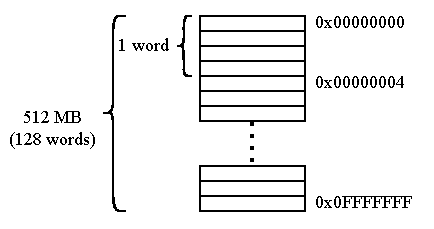
\includegraphics[width=.7\textwidth]{img/diagrams/ram.pdf}
		\caption{\texttt{RAM} implementation as a continuous piece of memory}
		\label{RAM implementation as a continuous piece of memory}
	\end{figure}
	
	A more effective approach would involve dynamically allocating fragmented pieces of memory as they are being addressed by the \texttt{CPU}. However, the author would argue that such an implementation would be algorithmically more complex, which could lead to distracting errors when implementing memory-related instruction, especially in the early stages of development. As a result, it was classified as a \textit{nice-to-have} feature that would be worth addressing in the future once the emulator has been thoroughly \texttt{QA}-tested.
	
	\newpage
	
	\subsubsection{Debug Monitor} \label{section-Debug-Monitor}
	
	The debug monitor plays the role of a memory-mapped output device for displaying \texttt{8-bit} character-based information.
	
	\begin{important}
		This component is not included in Raspberry Pi Zero itself; its presence serves solely for debugging purposes during the development of ZeroMate.
	\end{important}
	
	The ZeroMate project also includes a basic driver for the debug monitor that the user can seamlessly integrate into their build system. As showcased in Listing \ref{Demonstration of the use of the debug monitor}, this allows them to use \textbf{\say{print-like} functions} they might be familiar with from high-level programming languages, which may result in easier troubleshooting and resolving errors.
	
\begin{code}{C++}{Demonstration of the use of the debug monitor \label{Demonstration of the use of the debug monitor}}
#include "monitor.h"

int main() {
	bool flag = false;
	unsigned int my_var = 155;
	
	sMonitor << "Hello World\n";
	sMonitor << "myVar = " << my_var << '\n';
	sMonitor << "flag = " << flag << '\n';
	
	return 0;
}
\end{code}
	
	\begin{figure}[ht]
		\centering
		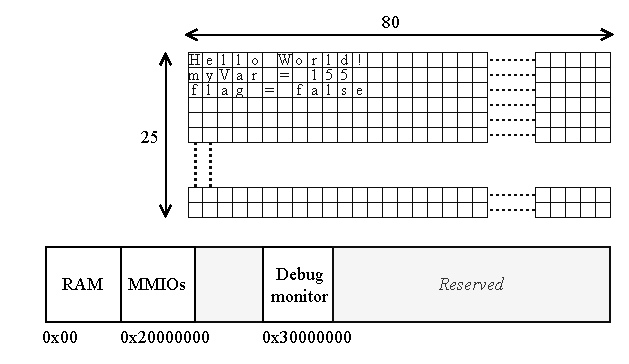
\includegraphics[width=0.96\textwidth]{img/diagrams/debug_monitor.pdf}
		\caption{Memory-mapped debug monitor}
		\label{Memory-mapped debug monitor}
	\end{figure}
	
	To attain the same capabilities in practice, the user would need to utilize a form of serial communication, such as \texttt{UART}, through which they could transmit characters to an external device \footnote{While there are alternative methods to achieve the same functionality, this approach is among the most common ones.}. This is commonly achieved by running software like \textit{PuTTY} \cite{putty} on the user's computer.
	
	As shown in Figure \ref{Memory-mapped debug monitor}, the debug monitor is mapped to an unoccupied address \texttt{0x30000000}. It is structured as a flat memory region, which is managed by the driver the user code interacts with. Inspired by the standard terminal text mode, the size of the monitor was chosen to be \texttt{80x25 8-bit} characters \footnote{From an implementation point of view, it could vary in size as long as it does not overlap with other memory regions.}.
	
	\subsubsection{True Random Number Generator} \label{trng}
	The \texttt{TRGN} peripheral is an integrated \texttt{32-bit} hardware random number generator. Although it is not documented in the official \texttt{BCM2835} manual \cite{BCM2835}, its existence can be confirmed, for instance, by examining the implementation in the GNU/Linux kernel \cite{trng}.
	
	For simplification purposes, ZeroMate primarily focuses on providing random numbers while omitting more advanced features such as configuring the generator's speed, generating interrupts, or the warm-up count. The warm-up count refers to the process of generating and immediately discarding a set of random numbers before the initialization is completed \footnote{The initial values are \say{less random}.}.
	
	From the user's code perspective, the process of \textbf{retrieving a random number consists of two steps}, which are displayed in Figure \ref{Reading random numbers using the TRNG peripheral}.
	
	\begin{figure}[ht]
		\centering
		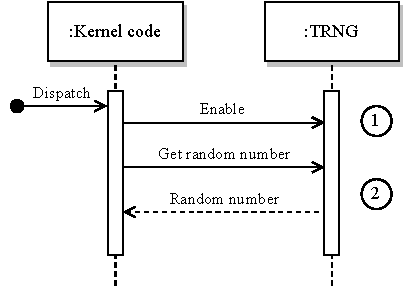
\includegraphics[width=.6\textwidth]{img/diagrams/trng.pdf}
		\caption{Reading random numbers from the \texttt{TRNG} peripheral}
		\label{Reading random numbers using the TRNG peripheral}
	\end{figure}
	
	\newpage
	
	\paragraph{Enabling \texttt{TRNG}}
	
	The \texttt{TRNG} peripheral is enabled by setting bit 0 of the \textbf{control register} to \texttt{1}. If implemented, this action would also trigger the processing of \say{warming up}, which was mentioned previously.
	
	\paragraph{Reading random numbers}
	
	First, the user should check the availability of random numbers in the \texttt{TRNG}'s queue by examining the most significant 8 bits of the \textbf{status register}. If this number is 0, they should wait until the generator accumulates a sufficient amount of entropy to generate a random number. When data is ready, reading from the \textbf{data register} will retrieve a random number from the queue.
	
	\begin{important}
		ZeroMate can almost instantly generate a random number using a pseudo-random number generator. As a result, when reading the most significant 8 bits of the status register, the user will consistently receive the value 1, meaning they can read random numbers without delay, which could potentially be another area for future improvements.
	\end{important}
	
	\textbf{Utilizing a pseudo-random number generator}, such as an \textit{LCG} \cite{lcs} or \textit{Mersenne-Twister}, \textbf{can greatly improve the performance of the emulation}. Depending on the implementation, accessing a true random number generator via the host operating system may have a detrimental impact on overall speed, as it may continually gather entropy from user inputs, like key presses or cursor movements. This can potentially lead to a blocking operation if there is currently insufficient entropy available.
	
	\subsubsection{\texttt{ARM} Timer} \label{ARM Timer}
	
	One of the most frequently used functions of the \texttt{ARM} timer is to periodically trigger interrupts, whether it is for toggling an \texttt{LED}, generating a \texttt{PWM} signal, or switching the current \texttt{CPU} context, which is an integral part of any preemptive \texttt{OS} scheduler.
	
	As shown in Figure \ref{Context of the ARM timer component}, there are two data/control paths through which the timer can be interacted with. The first path, when the timer is treated as a memory-mapped peripheral, serves the purpose of reading from and writing to its internal registers in order to configure its desired functionality. This may involve steps such as setting up the prescaler, enabling interrupts, or defining the initial threshold value. The other path is used implicitly by the \texttt{CPU} to notify the peripheral about how many \texttt{CPU} cycles it took to execute the last instruction. The \texttt{ARM} timer then leverages the prescaler to divide the input frequency, as the main \texttt{CPU} frequency may not always be suitable for the given task.
	
	\newpage
	
	\begin{important}
		As far as ZeroMate is concerned, all time-related functionalities, such as the \texttt{ARM} timer, \texttt{UART}, or \texttt{I\textsuperscript{2}C}, are for synchronization purposes, inherently derived from the emulated \texttt{CPU}'s clock.
	\end{important}
	
	\begin{figure}[ht]
		\centering
		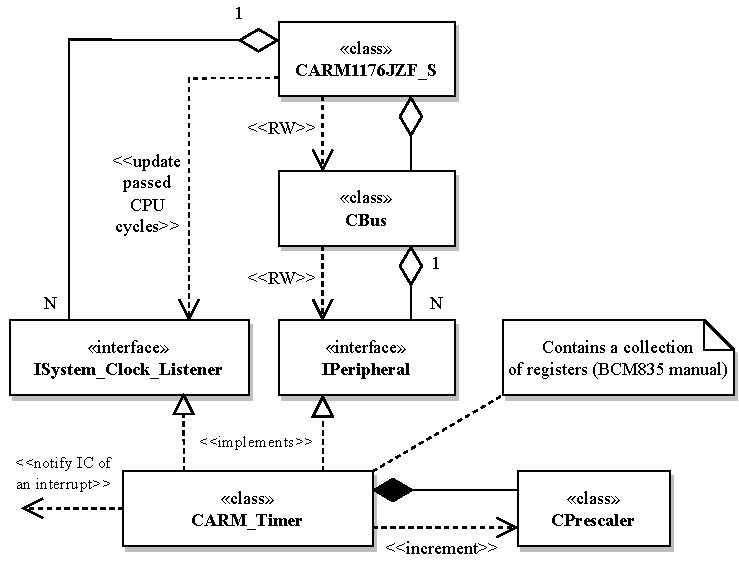
\includegraphics[width=1.0\textwidth]{img/diagrams/arm_timer.pdf}
		\caption{Context of the \texttt{ARM} timer component}
		\label{Context of the ARM timer component}
	\end{figure}
	
	As stated previously, the purpose of the prescaler is to divide the \texttt{CPU}'s frequency by a factor of 1, 16, or 256, which ultimately affects the timer's period - how rapidly the \textbf{value register} counts down to zero. Additionally, the timer's period can be adjusted by modifying the value in the \textbf{load register}, which serves to re-initialize the value register whenever it reaches zero. If enabled, with each such event, the timer will trigger an interrupt. This concept is visualized in Figure \ref{Content of the value register of the ARM timer over time}.
	
	\begin{figure}[ht]
		\centering
		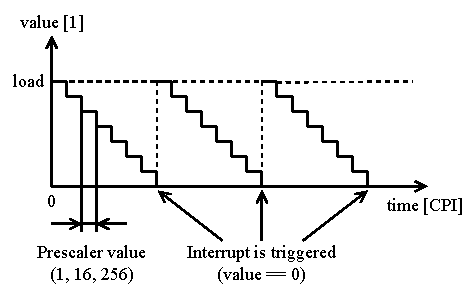
\includegraphics[width=.8\textwidth]{img/diagrams/arm_timer_2.pdf}
		\caption{Content of the value register of the \texttt{ARM} timer over time}
		\label{Content of the value register of the ARM timer over time}
	\end{figure}
	
	\newpage
	
	\subsubsection{General Purpose Input/Output}
	
	The \texttt{GPIO} manager is a peripheral that manages the \textbf{54 general-purpose input-output pins} that are available to the programmer. These \texttt{GPIO} pins also function as a connecting interface for all external devices, which is shown in Figure \ref{Internal vs External peripherals}. Each pin can be represented as a separate class encapsulating its current state, which consists of the pin's function, a list of enabled interrupts, an indication of any pending interrupts, and its current state.
	
	\begin{figure}[ht]
		\centering
		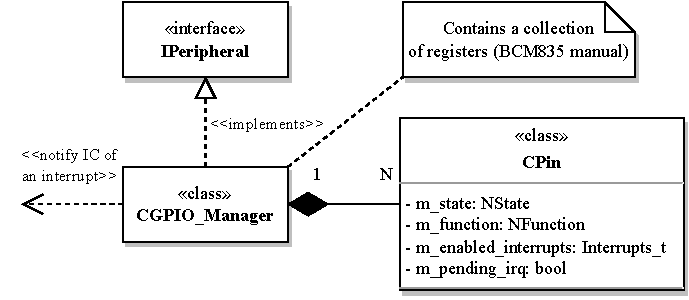
\includegraphics[width=0.95\textwidth]{img/diagrams/gpio_manager.pdf}
		\caption{Structure of the \texttt{GPIO} manager\protect\footnotemark}
		\label{Structure of the GPIO manager}
	\end{figure}
	
	\footnotetext{The \texttt{CPin} class also exposes a set of public functions (getters/setters) that allow the caller to access its private data members.}
	
	All \texttt{GPIO} pin functions, as well as interrupt types, can be found explained in the \texttt{BCM2835} manual \cite{BCM2835}.
	
	The pin's function restricts the way the pin can be interacted with. For instance, when the user tries to read from an output pin, they will be prompted with a warning message indicating that their action is inconsistent with the current pin configuration.
	
	\begin{important}
		ZeroMate does not provide support for analog pins. Therefore, all \texttt{GPIO} pins mentioned in this document are regarded as digital pins, with only two possible states - \texttt{HIGH} and \texttt{LOW}. To accommodate analog signals, the \texttt{GPIO} controller would need to be extended by an additional piece of information indicating whether a pin is digital or analog to  either hold a \texttt{bool} or \texttt{signed integer} value respectively \footnote{In reality, the \texttt{GPIO} controller routes analog pins to the \texttt{ADC}, or \textit{Analogue to Digital Converter}, which is another internal peripheral of Raspberry Pi Zero.}.
	\end{important}
	
	\paragraph{Emulation of latches}
	
	\textbf{Some of the \texttt{GPIO} registers work, on a hardware level, as latches}, which may not be as intuitive from a software emulation point of view. An example of this principle would be the \texttt{GPSETx} and \texttt{GPCLRx} registers, which respectively set an output pin to a logical one and zero. These registers are stateless, meaning they do not retain their previous state internally. As shown in Listing \ref{SW emulation of a HW latch register}, one approach to emulate such behavior is to reset the register to its default value after a write operation has been performed.
	
\begin{code}{C++}{\texttt{SW} emulation of a \texttt{HW} latch register \label{SW emulation of a HW latch register}}
void Set_Pin_High(std::uint32_t& gpset0)
{
	// Iterate over all bits of gpset0.
	// If gpset0[i]==1, then set the 
	// corresponding pin to HIGH.
	
	gpset0 = 0; // SW latch emulation
}
\end{code}
	
	\paragraph{Detecting Interrupts}
	
	Whenever the state of a pin changes, a series of checks is performed to determine whether an interrupt has occurred. One of the most commonly used types of interrupts is triggered by a change in the logical value of a specific pin, either transitioning from \texttt{HIGH} to \texttt{LOW} or vice versa. The types of interrupt to be detected for each pin can be specified in the corresponding registers. When an interrupt is detected, it is reported to the interrupt controller, which can then initiate further actions, which is captured in Figure \ref{Structure of the GPIO manager}.
	
	\newpage
	
	\subsubsection{Interrupt Controller}
	
	As shown in Figure \ref{Context of the interrupt controller}, the interrupt controller serves as the primary interface for managing all peripherals that can generate interrupts. Through the interrupt controller, users can enable or disable various interrupt sources, including \texttt{GPIO} pins, the \texttt{ARM} timer, and the \texttt{UART} peripheral. \textbf{When an interrupt is signaled to the interrupt controller, it checks whether the source is enabled; otherwise, the event is discarded}. From the \texttt{CPU}'s point of view, after an instruction has been executed, it checks with the interrupt controller to ascertain the existence of any pending interrupts. If the interrupt controller has a record of a pending interrupt, and global interrupts are enabled, the \texttt{CPU} proceeds to throw an \texttt{IRQ} exception.
	
	\begin{figure}[ht]
		\centering
		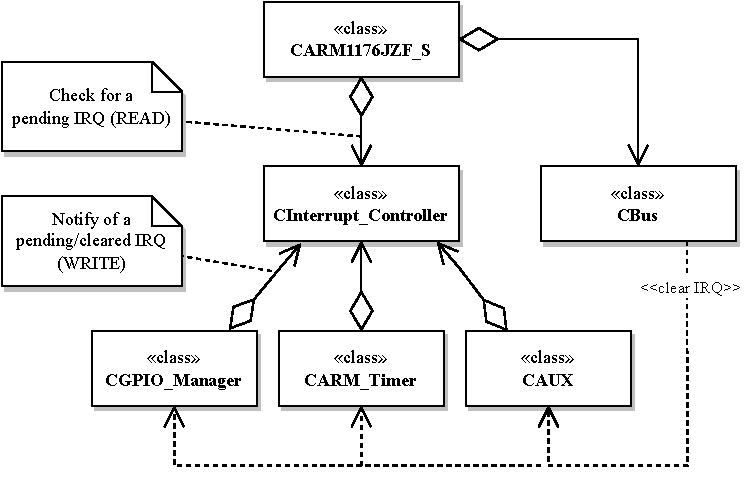
\includegraphics[width=0.95\textwidth]{img/diagrams/interrupt_controller.pdf}
		\caption{Context of the interrupt controller}
		\label{Context of the interrupt controller}
	\end{figure}
	
	In terms of design, the interrupt controller encapsulates an associative storage that pairs each \texttt{IRQ} source \footnote{The reader can find a list of all available \texttt{IRQ} sources in the \texttt{BCM2835} datasheet \cite{BCM2835}.} with its associated metadata, indicating whether it is enabled and if there is a pending interrupt. From the \texttt{CPU}'s perspective, this storage, which is shown in Figure \ref{Encapsulated information about IRQ sources}, is read-only, as its sole purpose is to check for any pending interrupts. The contents of this storage are modified by the peripherals themselves, either when they generate an interrupt or clear a pending interrupt.
	
	\begin{important}
		As noted in Chapter \ref{chapter-ARM Architecture}, an ARM processor also features so-called fast interrupts, or \texttt{FIQ} for short. However, ZeroMate does not offer support for it as it primarily focuses on fundamental principles rather than more advanced features.
	\end{important}
	
	\newpage
	
	\begin{figure}[ht]
		\centering
		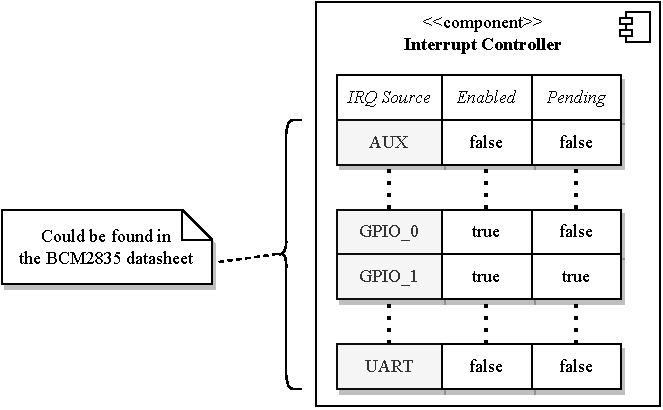
\includegraphics[width=0.87\textwidth]{img/diagrams/irq_sources.pdf}
		\caption{Encapsulated information about \texttt{IRQ} sources}
		\label{Encapsulated information about IRQ sources}
	\end{figure}
	
	It is worth mentioning that the interrupt controller of the \texttt{BCM2835} microcontroller distinguishes between two types of interrupt sources - \textit{Basic \texttt{IRQ}}, which are ARM-specific, and \textit{\texttt{IRQ}}, which are shared between the \texttt{GPU} and the \texttt{CPU}. Both types can be found listed in the \texttt{BCM2835} datasheet \cite{BCM2835}. Nevertheless, from a design perspective, the underlying principles remain the same.
	
	\subsubsection{Auxiliaries} \label{AUX}
	
	\textbf{The auxiliary peripheral comprises three distinct peripherals} - \texttt{Mini\_UART}, \texttt{SPI\_0}, and \texttt{SPI\_1}. Among these, only \texttt{Mini\_UART} is currently supported by ZeroMate.
	
	There are two primary registers shared among all auxiliary peripherals - the \texttt{enable} register, responsible for activating the respective peripheral, and the \texttt{IRQ} register, which signals pending interrupts. The remaining registers are specific to each peripheral, as depicted in Figure \ref{Registers of the AUX peripheral}.
	
	\begin{figure}[ht]
		\centering
		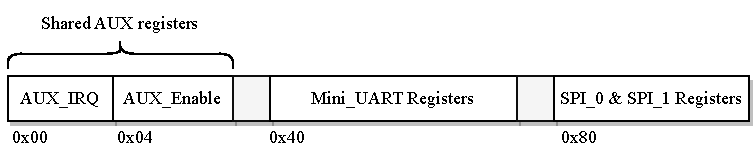
\includegraphics[width=0.95\textwidth]{img/diagrams/aux_reg.pdf}
		\caption{Registers of the \texttt{AUX} peripheral}
		\label{Registers of the AUX peripheral}
	\end{figure}
	
	Whenever a read/write request is received, using the technique described in Section \ref{Memory-mapped Registers}, the \texttt{AUX} class can efficiently redirect the execution to the relevant auxiliary peripheral, which will subsequently handle the request internally.
	
	\newpage
	
	\begin{figure}[ht]
		\centering
		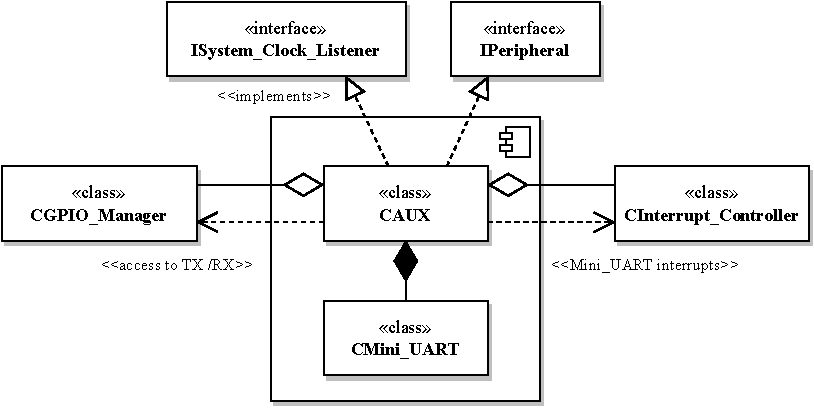
\includegraphics[width=0.98\textwidth]{img/diagrams/aux_peripheral.pdf}
		\caption{Structure of the \texttt{AUX} peripheral}
		\label{Structure of the AUX peripheral}
	\end{figure}
	
	Figure \ref{Structure of the AUX peripheral} shows the internal structure and dependencies of the \texttt{AUX} peripheral. It can be noticed that it implements the \texttt{ISystem\_Clock\_Listener} interface, whose purpose is described in Section \ref{System Clock Listener}, which allows it to synchronize with the rest of the system.
	
	\paragraph{\texttt{Mini\_UART}}
	
	\texttt{UART}, which stands for \textit{Universal Asynchronous Receiver-Transmitter}, inherently operates as asynchronous communication, which means there is no explicit synchronization between the two devices. Since these devices may have different clock speeds, they must adjust their frequencies to establish a common speed known as the \textbf{baudrate}, which expresses how many bits can be received/transmitted per second.
	
	\begin{figure}[ht]
		\centering
		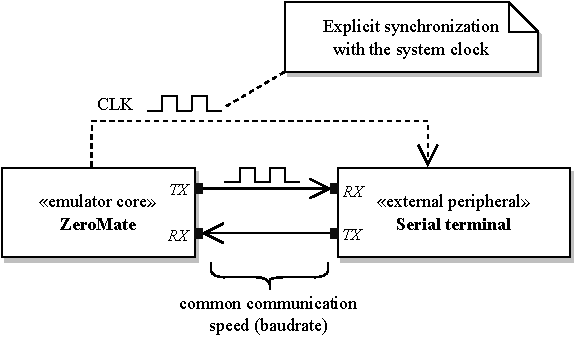
\includegraphics[width=0.8\textwidth]{img/diagrams/mini_uart_2.pdf}
		\caption{\texttt{UART} communication with an external peripheral}
		\label{UART communication with an external peripheral}
	\end{figure}
	
	The \texttt{BCM2835} microcontroller does not incorporate a full version of \texttt{UART}. Instead, it supports a simplified version known as \texttt{Mini\_UART}, which omits some of the extended features. As a result, the user is only able to modify the baudrate and the number of data bits transferred within a single frame, which can be either seven or eight. The remaining parameters, such as parity and the number of stop bits, are fixed according to the datasheet \cite{BCM2835}.
	
	\begin{important}
		In ZeroMate, all external peripherals are provided read-only access to the system clock, enabling them to synchronize themselves if required. This approach, depicted in Figure \ref{UART communication with an external peripheral}, contradicts the fundamental principles of asynchronous communication since it introduces a form of synchronization. However, this design choice was made to enhance the emulation's reliability while still enabling users to utilize \texttt{Mini\_UART} as if they were interacting with real hardware.
	\end{important}
	
	The implementation of \texttt{Mini\_UART} communication can be accomplished through a state machine driven by a pre-divided system clock, as shown in Figure \ref{Mini_UART state machine}. When a predefined number of \texttt{CPU} cycles have passed, the state machine updates itself to transmit and receive the next bit of the current data frame, which can be seen in Figure \ref{Example of a Mini_UART data frame with 8 bits of data} \footnote{Transmitting a single bit can be done by setting the corresponding \texttt{TX} pin to the desired value. Further details on what \texttt{GPIO} pins are designated for \texttt{Mini\_UART} can be found in the datasheet \cite{BCM2835}.}.
	
	\begin{figure}[ht]
		\centering
		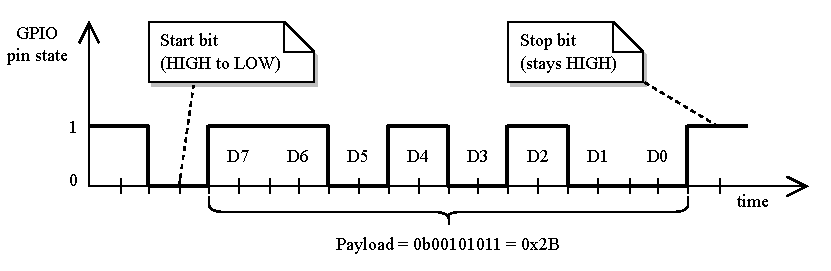
\includegraphics[width=1.0\textwidth]{img/diagrams/mini_uart.pdf}
		\caption{Example of a \texttt{Mini\_UART} data frame with 8 bits of data}
		\label{Example of a Mini_UART data frame with 8 bits of data}
	\end{figure}
	
	Receiving data can be implemented in a similar manner. Instead of setting the value of the \texttt{TX} pin, the state machine reads the value of the \texttt{RX} pin, which has been set previously by an external peripheral.
	
	\newpage
	
	\begin{figure}[ht]
		\centering
		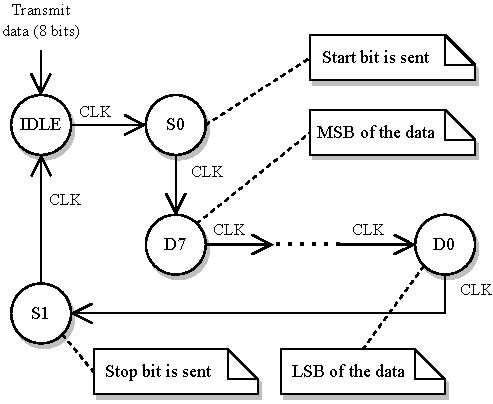
\includegraphics[width=0.6\textwidth]{img/diagrams/mini_uart_state_machine.pdf}
		\caption{\texttt{Mini\_UART} state machine (transmitting 8 bits)}
		\label{Mini_UART state machine}
	\end{figure}
	
	\subsubsection{Broadcom Serial Controller} \label{BSC}
	
	The Broadcom serial controller, often abbreviated as \texttt{BSC}, is a peripheral device that allows the user to communicate with external devices, usually sensors, using the \texttt{I\textsuperscript{2}C} protocol, which is a synchronous serial communication standard. \texttt{I\textsuperscript{2}C} utilizes two \texttt{GPIO} pins - \texttt{SDA} for data transmission and \texttt{SCL} for synchronization. Raspberry Pi Zero is equipped with three of these devices that can be found mapped to their respective addresses in Figure \ref{BCM2835 memory layout emulated by ZeroMate}.
	
	From a design point of view, the emulation of an \texttt{I\textsuperscript{2}C} bus is nearly identical to \texttt{UART}, with the primary distinctions being the frame structure and the synchronous transmission of individual bits using an additional \texttt{GPIO} pin instead of the emulated \texttt{CPU} clock.
	
	\begin{important}
		While there are various configurations of the \texttt{I\textsuperscript{2}C} communication protocol \footnote{They vary in voltage levels for representing logical 1 and 0, as well as in how they define the start and stop bits using the \texttt{SDA} and \texttt{SCL} signals.}, ZeroMate exclusively supports only one, which is presented in Figure \ref{Structure of an I2C frame}. As stated previously, ZeroMate emphasizes the emulation of fundamental principles, rather than attempting to implement every conceivable configuration, which would only add unnecessary complexity without delivering any added value.
	\end{important}
	
	\newpage
	
	\begin{figure}[ht]
		\centering
		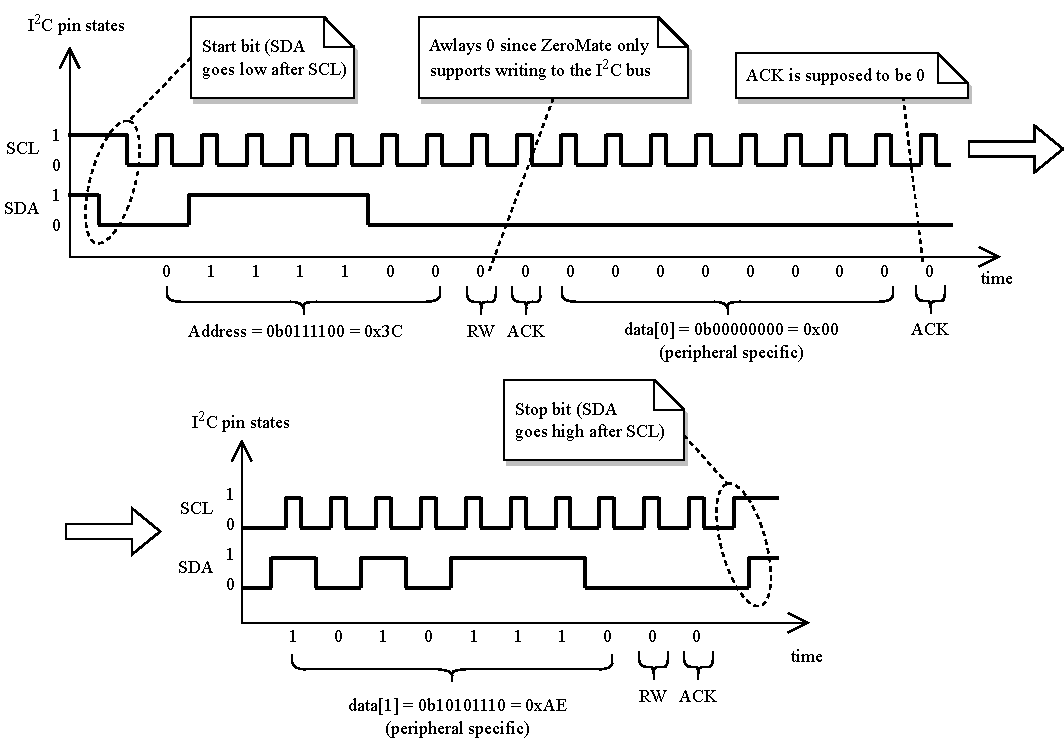
\includegraphics[width=1.0\textwidth]{img/diagrams/bsc.pdf}
		\caption{Structure of an \texttt{I\textsuperscript{2}C} frame}
		\label{Structure of an I2C frame}
	\end{figure}
	
	The ZeroMate emulator comes with several standalone external peripherals that employ the same communication interface. Users can connect these peripherals to the system based on their preferences using a configuration file, which is further discussed in Section \ref{External Peripherals}.
	
	\subsection{\texttt{ARM1176JZF\_S}}
	
	\textbf{All the previously mentioned peripherals are not self-sufficient in operation}; they require external control. This is where \texttt{ARM1176JZF\_S}, which serves as the central processing unit in the \texttt{BCM2835} microcontroller, comes into play, as it executes individual \texttt{32-bit} \texttt{ARM} instructions that may utilize these peripherals in various ways.
	
	In terms of architecture, the \texttt{ARM1176JZF\_S} component is divided into several tightly integrated building blocks, as shown in Figure \ref{Internal components of the ARM1176JZF_S processor}, to maintain a structured and organized design. The subsequent sections detail how each of these sub-peripherals contributes to the overall emulation of the \texttt{ARM1176JZF\_S} processor.
	
	\newpage
	
	\begin{figure}[ht]
		\centering
		\includegraphics[width=1.0\textwidth]{img/diagrams/arm1176jzf_s.pdf}
		\caption{Internal components of the \texttt{ARM1176JZF\_S} processor}
		\label{Internal components of the ARM1176JZF_S processor}
	\end{figure}
	
	\subsubsection{Central Processing Unit Context}
	
	\textbf{The \texttt{CPU} context functions as an encapsulation of the current state of the \texttt{CPU}}, including details such as the current contents of the registers and the active \texttt{CPU} mode. It is designed to provide an interface for accessing registers, enabling transitions between different modes, and offering other utility functions that abstract the underlying low-level logic, such as reading the state of individual bits of the \textit{Current Program Status Register}, which are shown in Figure \ref{Current Program Status Register}. From a design standpoint, its relationship with the \texttt{CPU} core is captured in Figure \ref{Relationship between the CPU context and the CPU core}.
	
	\begin{figure}[ht]
		\centering
		\includegraphics[width=0.8\textwidth]{img/diagrams/cpu_context.pdf}
		\caption{Relationship between the \texttt{CPU} context and the \texttt{CPU} core}
		\label{Relationship between the CPU context and the CPU core}
	\end{figure}
	
	\paragraph{Bank Registers}
	
	One of the presented challenges involves implementing so-called \textit{bank} registers, where, as mentioned in Section \ref{section-banked-registers}, each \texttt{CPU} mode possesses its distinct subset of registers that are automatically loaded when the mode changes. Additional information regarding this topic is available in Section A2.3 of the official ARM Architecture Reference Manual \cite{ARM_reference_manual}. 
	
	As illustrated in Listing \ref{Retrieving a CPU register}, one approach to address this challenge involves creating a lookup table for all bank registers within each \texttt{CPU} mode, effectively replacing the ones used in the \textit{User/System} mode, which are otherwise used by default.
	
	%\begin{figure}[ht]
	%\centering
	%\includegraphics[width=0.9\textwidth]{img/diagrams/bank_registers.pdf}
	%\caption{Bank registers lookup table}
	%\label{Bank registers lookup table}
	%\end{figure}
	
\begin{code}{c++}{Retrieving a \texttt{CPU} register \label{Retrieving a CPU register}} 
uint32_t& Get_Register(uint32_t idx, NCPU_Mode mode) 
{
	// Check if a banked register should be returned
	if (m_banked_regs.at(mode).contains(idx))
		return m_banked_regs[mode][idx];
	
	// A non-banked register is being addressed
	return m_banked_regs[NCPU_Mode::System][idx];
}
\end{code}
	
	\paragraph{Control Registers}
	
	The \textit{Current Program Status Register} and the \textit{Saved Program Status Registers}, commonly known as the \texttt{CPSR} and \texttt{SPSR} registers, are implemented in a similar way, with each \texttt{CPU} mode having its designated pair of these registers.
	
	\subsubsection{Instruction Set Architecture Decoder}
	
	\textbf{The primary role of the instruction set architecture decoder, abbreviated as the \texttt{ISA} decoder, is to analyze a \texttt{32-bit} value and ascertain the type of the ARM instruction it represents}, so it could be treated and decoded accordingly. This task must be executed with the utmost efficiency, as it is repetitively performed for each instruction the \texttt{CPU} executes.
	
	In the case of the emulated \texttt{CPU}, the \texttt{ISA} decoder functions as a \say{black box} offering a single-function interface, as demonstrated in Listing \ref{Interface of the ISA decoder} below.
	
\begin{code}{C++}{Interface of the \texttt{ISA} decoder\label{Interface of the ISA decoder}}
// Returns the type of a given 32-bit ARM instruction
[[nodiscard]] static CInstruction::NType 
Get_Instruction_Type(uint32_t instruction) noexcept;
\end{code}
	
	The typical and sole use-case of this interface is further illustrated in the sequence diagram shown in Figure \ref{Use of the ISA decoder by the CPU}. In this diagram, the \texttt{CPU} fetches the next instruction from \texttt{RAM} and employs the \texttt{ISA} decoder to determine its type, enabling it to proceed with the execution.
	
	\newpage
	
	\begin{figure}[ht]
		\centering
		\includegraphics[width=1.0\textwidth]{img/diagrams/isa_decoder.pdf}
		\caption{Use of the \texttt{ISA} decoder by the \texttt{CPU}}
		\label{Use of the ISA decoder by the CPU}
	\end{figure}
	
	Internally, the \texttt{ISA} decoder maintains a look-up table of instructions masks that are sequentially applied to the given \texttt{32-bit} value until the operation's result matches the expected value associated with the current mask. Each mask serves the purpose of zeroing out the variable bits specific to the instruction, leaving only the known bits in place, the expected value, which is then used to unambiguously determine the type of instruction.
	
	\begin{figure}[ht]
		\centering
		\includegraphics[width=0.75\textwidth]{img/diagrams/isa_decoder_2.pdf}
		\caption{Algorithm for decoding \texttt{ARM} instructions}
		\label{Algorithm for decoding ARM instructions}
	\end{figure}
	
	\newpage
	
	Figure \ref{Algorithm for decoding ARM instructions} shows the algorithm for decoding \texttt{ARM} instructions, which, in the worst-case scenario, operates with time complexity of $\mathcal{O}(n)$, where $n$ represents the size of the look-up table. \textbf{To ensure unambiguous decoding, it is essential to test the bit masks in a specific order, starting with the most restrictive one and proceeding to the least restrictive one, based on the number of bits set within each mask}. Otherwise, there might be a risk of incorrectly identifying the instruction type, inevitably leading to unexpected behavior.
	
	Once an instruction has been classified, the \texttt{32-bit} value can be encapsulated within its corresponding class representation, providing an interface to access the specific fields relevant to that instruction. The contents of the look-up table can be constructed using resources such as the B2 Appendix authored by Andrew Sloss and Chris Wright, which provides ARM instruction encodings \cite{B2_appendix}. 
	
	\subsubsection{Exceptions} \label{Exceptions}
	
	Exceptions can originate from various components within the ZeroMate emulator. These exceptions may arise from factors such as the absence of an addressed page, unaligned memory access, or the execution of a privileged instruction in the unprivileged \texttt{CPU} mode. ZeroMate handles ARM \texttt{CPU} exceptions as runtime errors on the host machine. As a result, the emulated \texttt{CPU} core must be prepared for the possibility that the currently executing instruction may abruptly trigger an exception that must be properly handled. Figure \ref{Hierarchy of the CPU exceptions} shows the hierarchy of \texttt{CPU} exceptions, where each class may include additional information pertaining to the exception, such as a descriptive message, the address at which it occurred, or the address of the vector associated with that specific exception, which is shown in Table \ref{List of ARM CPU exceptions}.
	
	\begin{figure}[ht]
		\centering
		\includegraphics[width=0.9\textwidth]{img/diagrams/exceptions.pdf}
		\caption{Hierarchy of the \texttt{CPU} exceptions}
		\label{Hierarchy of the CPU exceptions}
	\end{figure}
	
	\newpage
	
	\subsubsection{Arithmetic-Logic Unit}
	
	As the name suggests, the arithmetic-logic unit, also known as the \texttt{ALU}, is \textbf{responsible for carrying out arithmetic and logical operations}, such as \textit{addition}, \textit{subtraction}, \textit{comparison}, etc. 
	
	From a design standpoint, the \texttt{ALU} can be envisioned as a set of collaborative functions concealed behind a single function interface, which is made accessible to the central processing unit as shown in Figure \ref{Architectural structure of the ALU}.
	
	\begin{figure}[ht]
		\centering
		\includegraphics[width=0.75\textwidth]{img/diagrams/alu.pdf}
		\caption{Architectural structure of the \texttt{ALU}}
		\label{Architectural structure of the ALU}
	\end{figure}
	
	As illustrated in Figure \ref{Architectural structure of the ALU} above, when the \texttt{ALU} is employed, the \texttt{CPU} must provide the current state of its flags as well as the data processing instruction currently in execution, which is then internally analyzed by the \texttt{ALU} to determine the specific type of operation to be carried out.
	
	\paragraph{\texttt{MAC} Unit}
	
	The \texttt{ARM1176JZF\_S} also incorporates a module referred to as \texttt{MAC}, specifically designed for performing a variety of \textbf{multiplication operations}. These operations can involve the multiplication of either signed or unsigned \texttt{32-bi}t integers, signed or unsigned \texttt{64-bit} integers, or multiplication with addition, where a third value is added to the result of a multiplication. All instruction encodings can be found in the B2 Appendix document \cite{B2_appendix}. From an implementation perspective, it can be integrated in a manner similar to the \texttt{ALU}.
	
	\subsubsection{Memory Management Unit}
	
	If enabled, the memory management unit, often referred to as the \texttt{MMU}, comes into play just before the \texttt{CPU} sends a read/write request to the system bus. As shown in Figure \ref{BCM2835 address translation processes}, \textbf{its primary function is to convert a \texttt{32-bit} virtual address into a corresponding \texttt{32-bit} physical address} based on the information stored in the corresponding page table, allowing the user to reorganize the address space to their needs. Furthermore, it performs a series of checks, the failure of which could result in a \texttt{MMU} abort \footnote{Users of the x86 architecture might already be acquainted with the concept of a \textit{page fault}, which, in this context, can be thought of in a similar way.}.
	
	\begin{enumerate}
		\item In the initial step, the \texttt{MMU} retrieves the page associated with the address from the first-level page table to ascertain its type. This type indicates whether it references a nested second-level page table or a physical frame. In the latter case, the \texttt{MMU} also confirms the page's presence in \texttt{RAM}, as it might have been swapped out, for example, to a file.
		
		\item When addressing a physical frame, the \texttt{MMU} checks access privileges of the target frame based on the current mode of the \texttt{CPU} in order to ensure that no security policy is being violated.
	\end{enumerate}
	
	If all checks have successfully passed, the \texttt{MMU} proceeds to convert the virtual address into a corresponding physical address. More detailed information about how the \texttt{MMU} operates can be found in Chapter 6 of the \texttt{ARM1176JZF\_S} Technical Reference Manual \cite{ARM1176JZF-S}.
	
	\begin{important}
		The ZeroMate emulator lacks support for nested page tables, which inevitably introduces certain limitations in the emulation. As a result, it utilizes a first-level page table that spans over the entire address space.
	\end{important}
	
	\begin{figure}[ht]
		\centering
		\includegraphics[width=1.0\textwidth]{img/diagrams/mmu.pdf}
		\caption{Utilization of the \texttt{MMU} when processing a \texttt{RW} request}
		\label{Utilization of the MMU when processing a RW request}
	\end{figure}
	
	Placing an emphasis on the Memory Management Unit, Figure \ref{Utilization of the MMU when processing a RW request} illustrates the essential steps to be taken when executing a read/write instruction. Whenever the address of page table 0 changes in the \texttt{TTBR\_0} register, the \texttt{MMU} retrieves the entire page table from \texttt{RAM} and stores it within its private data structure. This approach eliminates the need to repeatedly read it with each memory access, which would otherwise negatively impact the overall performance of the emulation. Once a physical address is obtained, the \texttt{CPU} can then proceed with the request.
	
	\paragraph{Implementation}
	
	As shown in Figure \ref{Structure of the first-level page table}, the implementation of a first-level page table can be tacked as an array of 4096 classes called \texttt{CPage}\footnote{Assuming the page granularity is \texttt{1MB}, covering the entire \texttt{4GB} address space requires 4096 page table entries.}. These classes serve as an abstraction for accessing individual fields of individual pages, where each page is represented as a \texttt{32-bit} value.
	
	\begin{figure}[ht]
		\centering
		\includegraphics[width=1.0\textwidth]{img/diagrams/page_table.pdf}
		\caption{Structure of the first-level page table}
		\label{Structure of the first-level page table}
	\end{figure}
	
	\paragraph{Translation Lookaside Buffer}
	
	Once a virtual address undergoes the process of translation, it is stored, along with its corresponding physical address, in a look-up table \footnote{It can be implemented, for instance, as an \texttt{std::unordered\_map<uint32\_t, uint32\_t>}}. In a real system, this table is known as the \textit{Translation Lookaside Buffer}, or \texttt{TLB} for short. The next time the same address is used, it does not have to go through the translation process again, which enhances performance. When a request is made to invalidate the \texttt{TLB} through the \textit{System Control Co-processor}, ZeroMate clears this associative data structure to prevent invalid addressing across various virtual address spaces.
	
	\newpage
	
	\subsubsection{Central Processing Unit Core} \label{Central Processing Unit Core}
	
	The central processing unit utilizes the functionality of all previously mentioned components. In terms of design, it is composed of multiple private member functions that are invoked based on the type of instruction currently being executed. These functions can be seen as microprograms, as they handle the specific operations associated with the current instruction.
	
	\begin{figure}[ht]
		\centering
		\includegraphics[width=1.0\textwidth]{img/diagrams/cpu_core.pdf}
		\caption{Execution loop of the emulated \texttt{CPU}\protect\footnotemark}
		\label{Execution loop of the emulated CPU}
	\end{figure}
	
	\footnotetext{The timestamp points serve as markers for performance measurement, which is further discussed in Chapter \ref{chapter-Performance-Evaluation}.}
	
	As shown in Figure \ref{Execution loop of the emulated CPU}, the microprograms are called within an infinite loop known as the execution loop, which fetches the next instruction from \texttt{RAM}, decodes it using the \texttt{ISA} decoder, and directs the execution to the appropriate microprogram responsible for carrying out the necessary steps to execute it. These steps may include tasks such as reading data from the stack, modifying register contents, utilizing the arithmetic-logic unit, and more.
	
	\begin{important}
		It is worth noting that a real system is significantly more complex than how ZeroMate implements it. However, the author would contend that any form of emulation involves trade-offs that result in the omission of certain details.
	\end{important}
	
	\paragraph{Catching Exceptions}
	
	As described in Section \ref{Exceptions}, the \texttt{CPU} must handle any exceptions that may arise during the execution of the current instruction. When an exception occurs, the \texttt{CPU} switches to the corresponding mode, saves the return address in the link register, as if it was invoking a function call, and sets the address of the next instruction to the value stored at the corresponding offset in the interrupt vector table.
	
	\paragraph{Updating \texttt{CPU} clock listeners}
	
	As discussed in Section \ref{System Clock Listener}, prior to moving on to the next instruction, the \texttt{CPU} informs all peripherals subscribed as system clock listeners about the number of \texttt{CPU} cycles required to execute the last instruction.
	
	\begin{important}
		While it is true that each instruction may require a varying number of \texttt{CPU} cycles for execution, in the current implementation, ZeroMate empirically averages this number to 8, which presents a potential area for future improvement. Users should be aware that the emulation speed does not match the speed of real hardware, and as a result, they may need to adjust timings in their firmware accordingly.
	\end{important}
	
	
	\subsection{Co-processors}
	
	As illustrated in Figure \ref{Component diagram of the CPU and its co-processors}, \textbf{ZeroMate takes into account two co-processors}, the design and functionality of which are described in the following two sections. Although their capabilities may be somewhat limited compared to what a real system offers, they serve the purpose of demonstrating the fundamental principles of interactions that can also be applied in practice.
	
	\begin{figure}[ht]
		\centering
		\includegraphics[width=0.9\textwidth]{img/diagrams/coprocessors.pdf}
		\caption{Component diagram of the \texttt{CPU} and its co-processors}
		\label{Component diagram of the CPU and its co-processors}
	\end{figure}
	
	\newpage
	
	As shown in Table \ref{List of ARM co-processor instructions}, the \texttt{CPU} communicates with individual co-processors through three types of instructions - \textit{data transfer}, \textit{register transfer}, and \textit{data operation}. When the emulated \texttt{CPU} detects a co-processor instruction, it does not perform any further analysis but promptly delegates it to the appropriate co-processor, determined by the \texttt{ID} encoded within the instruction itself. The co-processor then internally performs decoding and execution of the instruction using a technique similar to that used by the emulated \texttt{CPU}.
	
	Although the ZeroMate emulator currently accommodates only two co-processors, its overall design allows for a seamless integration of additional co-processors in the future, should the need arise. As shown in Figure \ref{Co-processor hierarchy}, the \texttt{CPU} maintains a collection of available co-processors, all of which implement the same interface, through which they are controlled by the \texttt{CPU}.
	
	\begin{figure}[ht]
		\centering
		\includegraphics[width=0.9\textwidth]{img/diagrams/coprocessors_2.pdf}
		\caption{Co-processor hierarchy}
		\label{Co-processor hierarchy}
	\end{figure}
	
	\subsubsection{Co-processor 15}
	
	As stated previously, the \textit{System Control Co-processor} comprises a tree-like hierarchy of \texttt{32-bit} registers that are used to enable a variety of additional features. These features include caching policy, branch prediction, unaligned memory access, setting up access to other co-processors, and so on \footnote{The list of all registers along with their functions can be found detailed in Chapter 3 of the \texttt{ARM1176JZF\_S} Technical Reference Manual \cite{ARM1176JZF-S}.}. As far as ZeroMate is concerned, its emulation efforts are directed primarily towards the registers listed in Table \ref{List of emulated CP15 registers}.
	
	\newpage
	
	\begin{center}
		\begin{longtable}{p{.12\textwidth}p{.12\textwidth}p{.10\textwidth}p{.52\textwidth}}
			\caption{List of emulated \texttt{CP15} registers}
			\label{List of emulated CP15 registers}\\
			\toprule[1.5pt]
			\textbf{Primary register} & \textbf{Secondary register} & \textbf{Index} & \textbf{Description}\\
			\midrule
			\endfirsthead
			\multicolumn{4}{c}{\tablename{}~\thetable{} \textit{(continued from the previous page)}}\\
			\midrule
			\textbf{Primary register} & \textbf{Secondary register} & \textbf{Index} & \textbf{Description}\\
			\midrule
			\endhead
			\midrule
			\multicolumn{4}{r}{\textit{(table continues on the next page)}}\\
			\endfoot
			\bottomrule[1.5pt]
			\endlastfoot
			%
			\texttt{C1} & \texttt{C0} & \texttt{0} & Control Register (see Table \ref{List of emulated flags of the CP15 control register})\\
			&  & \texttt{2} & Co-processor Access Control Register\\
			\midrule
			\texttt{C2} & \texttt{C0} & \texttt{0} & Translation Table Base Register 0 (\texttt{TTBR\_0})\\
			&  & \texttt{1} &Translation Table Base Register 1 (\texttt{TTBR\_1})\\
			&  & \texttt{2} & Translation Table Base Control\\
			\midrule
			\texttt{C8} & \texttt{C7} & \texttt{0} & Invalidate unified \texttt{TLB} unlocked entries\\
		\end{longtable}
	\end{center}
	
	Other frequently used \texttt{CP15} registers are implemented solely for the purpose of completeness, even though modifying them has no effect. If a user's firmware attempts to write to an unimplemented register, a warning message will be displayed, indicating this specific functionality is beyond the emulator's current capabilities.
	
	\begin{center}
		\begin{longtable}{p{.16\textwidth}p{.70\textwidth}}
			\caption{List of emulated flags of the \texttt{CP15} control register}
			\label{List of emulated flags of the CP15 control register}\\
			\toprule[1.5pt]
			\textbf{Bit position} & \textbf{Description}\\
			\midrule
			\endfirsthead
			\multicolumn{2}{c}{\tablename{}~\thetable{} \textit{(continued from the previous page)}}\\
			\midrule
			\textbf{Bit position} & \textbf{Description}\\
			\midrule
			\endhead
			\midrule
			\multicolumn{2}{r}{\textit{(table continues on the next page)}}\\
			\endfoot
			\bottomrule[1.5pt]
			\endlastfoot
			%
			\texttt{0} & Enables the \texttt{MMU}\\ 
			\texttt{13} & Determines the location of exception vectors\\ & (\texttt{0x00000000} vs \texttt{0xFFFF0000})\\ 
			\texttt{22} & Enables unaligned data access operations\\ 
		\end{longtable}
	\end{center}
	
	\newpage
	
	From an emulation perspective, \texttt{CP15} serves as an organized repository of information that is queried from within other components of the application, so they can, if required, adjust their designated actions accordingly. This hierarchical structure is visualized in Figure \ref{Design of the co-processor 15 register hierarchy}.
	
	\begin{figure}[ht]
		\centering
		\includegraphics[width=0.9\textwidth]{img/diagrams/cp15.pdf}
		\caption{Design of the co-processor 15 register hierarchy (uses primary register \texttt{C1} as an example)}
		\label{Design of the co-processor 15 register hierarchy}
	\end{figure}
	
	\subsubsection{Co-processor 10} \label{section-Co-processor-10}
	
	\textbf{Co-processor 10 allows users to work with single-precision (\texttt{32-bit}) floating-point numbers}. The design of this co-processor closely resembles that of the \texttt{CPU}, as illustrated in Figure \ref{Execution loop of the emulated CPU}. In this design, each instruction is first decoded and consequently executed within a private member function, which can be considered a microprogram.
	
	\begin{important}
		While ZeroMate supports most common vector floating-point instructions of version 2 (\texttt{VFPv2} \footnote{All \texttt{VFP} instruction can be found listed in Chapter C3 of the ARM Architecture Reference Manual \cite{ARM_reference_manual}.}), including \textit{addition}, \textit{subtraction}, \textit{multiplication}, \textit{division}, and \textit{square root}, it simplifies its implementation by omitting support for various rounding modes and floating-point exceptions. 
	\end{important}
	
	In terms of design, the floating-point unit, commonly denoted as the \texttt{FPU}, consists of an array of 32 internal registers, each 32 bits in size. Despite representing floating-point numbers, their underlining data type remains \texttt{uint32\_t}, enabling seamless data exchange between the \texttt{CPU} and the \texttt{FPU}.
	
	However, it is essential to emphasize that all operations must be executed as floating-point operations. As a result, the \texttt{32-bit} number can be encapsulated within a class that overrides its math operators, effectively hiding implementation details from the caller. Whenever an operation needs to be carried out, the register internally performs the following steps.
	
	\begin{enumerate}
		\item For all operands, convert the raw \texttt{32-bit} value into a \texttt{float} using the \texttt{IEEE 754} floating-point representation \cite{IEEE754}. This conversion can be accomplished through the helper member function shown in Listing \ref{Conversion between uint32_t and float}.
		\item Carry out the floating-point operation.
		\item Store the result back as a \texttt{uint32\_t} using the same technique demonstrated in Listing \ref{Conversion between uint32_t and float}.
	\end{enumerate}
	
\begin{code}{c++}{Conversion between \texttt{uint32\_t} and \texttt{float}\label{Conversion between uint32_t and float}}
template<typename Type>
[[nodiscard]] Type Get_Value_As() const
{
	return std::bit_cast<Type>(m_value); // since C++20
}
\end{code}
	
	\newpage
	
	\section{External Peripherals} \label{External 
		Peripherals}
	
	All the modules described previously form the core of the emulator, which is compiled as a standalone application. Furthermore, the \textbf{ZeroMate emulator offers a public single-header interface that enables the implementation of third-party external peripherals}, which can be compiled independently of the toolchain used for the core itself. In other words, users can choose their preferred programming language for developing an external peripheral, with the condition that they implement the interface and compile it as a shared library \footnote{The format of a shared library is \texttt{.dll} on Windows and \texttt{.so} on Linux, respectively.}. This concept is illustrated in Figure \ref{External peripheral interface}.
	
	Using a configuration file, these external peripherals can be then loaded by the core at runtime, enabling the user to create a custom circuit of external peripherals. Compiling as a shared library offers the advantage of creating multiple instances of the same peripheral. For instance, the user can employ multiple instances of \texttt{led.dll} to assemble a traffic light system, which can then be controlled by their custom firmware.
	
	\begin{figure}[ht]
		\centering
		\includegraphics[width=1.0\textwidth]{img/diagrams/external_peripherals.pdf}
		\caption{External peripheral interface}
		\label{External peripheral interface}
	\end{figure}
	
	\subsection{External Peripheral Interface}
	
	Upon construction, \textbf{every external peripheral is given access to the \texttt{GPIO}} pins, as it is their primary way of interaction with the core of the emulator. The interface also mandates that they implement a \texttt{Get\_GPIO\_Subscription} function, responsible for  returning a set of \texttt{GPIO} pins they wish to subscribe to \footnote{ZeroMate has support for connecting multiple external peripherals to the same \texttt{GPIO} pins, effectively creating a parallel connection.}. 
	
	Whenever the state of a \texttt{GPIO} changes, the emulator iterates over all external peripherals, examining their \texttt{GPIO} subscriptions, and duly informing them of the change. Additionally, they receive information about the number of \texttt{CPU} cycles it took to execute the last instruction, the same way internal peripherals do, effectively serving as an emulated replacement for an independent system clock.
	
	\begin{important}
		Certain external peripherals, such as a serial terminal, come with their own system clock. However, in ZeroMate, all timing functions are derived from the emulated \texttt{CPU} frequency.
	\end{important}
	
	Optionally, \textbf{they are provided access to the logging system}, which proves to be invaluable for debugging or providing insights into their current state. External peripherals are not obliged to implement a graphical user interface; nevertheless, they are implicitly provided with a context that they can utilize to render themselves within each frame.
	
	\subsection{Configuration}
	
	Upon startup, ZeroMate attempts to read a single configuration file in the \texttt{JSON} format that details the connections of external peripherals. Table \ref{Information stored in peripherals.json} outlines the obligatory fields that must be provided for every peripheral. ZeroMate handles the construction and management of all external peripherals within its dedicated address space on the host machine.
	
	\begin{center}
		\begin{longtable}{p{.16\textwidth}p{.35\textwidth}p{.35\textwidth}}
			\caption{Information stored in \texttt{peripherals.json}}
			\label{Information stored in peripherals.json}\\
			\toprule[1.5pt]
			\textbf{Field} & \textbf{Example} & \textbf{Description}\\
			\midrule
			\endfirsthead
			\multicolumn{2}{c}{\tablename{}~\thetable{} \textit{(continued from the previous page)}}\\
			\midrule
			\textbf{Bit position} & \textbf{Description}\\
			\midrule
			\endhead
			\midrule
			\multicolumn{2}{r}{\textit{(table continues on the next page)}}\\
			\endfoot
			\bottomrule[1.5pt]
			\endlastfoot
			%
			\texttt{name} & \texttt{"7-segment Display"} & Unique name associated with the peripheral\\ 
			\texttt{connection} & \texttt{[ 2, 3, 4 ]} & Set of \texttt{GPIO} pins the peripheral is connected to\\ 
			\texttt{lib\_dir} & \texttt{"peripherals"} & Directory where the shared library is held\\
			\texttt{lib\_name} & \texttt{"seven\_seg\_display"} & Name of the shared library\\
		\end{longtable}
	\end{center}
	
	\newpage
	
	Figure \ref{Illustration of connection of two parallel 7-segment displays} provides a visual representation of a custom connection that connects two 7-segment displays in parallel, having them simultaneously display the same piece of information.
	
	\begin{figure}[ht]
		\centering
		\includegraphics[width=0.75\textwidth]{img/diagrams/connection.pdf}
		\caption{Illustration of connection of two parallel 7-segment displays}
		\label{Illustration of connection of two parallel 7-segment displays}
	\end{figure}
	
	\subsection{Examples of External Peripherals}
	
	ZeroMate comes pre-packaged with several external peripherals, many of which mirror those found on the \texttt{DPP-01} board \cite{KIV-DPP-01}, which was designed for educational purposes within the KIV/OS class taught at the University of West Bohemia. Table \ref{List of emulated external DPP-01 peripherals} enumerates the external peripherals developed alongside the emulator.
	
	\begin{center}
		\begin{longtable}{p{.30\textwidth}p{.56\textwidth}}
			\caption{List of emulated external \texttt{DPP-01} peripherals}
			\label{List of emulated external DPP-01 peripherals}\\
			\toprule[1.5pt]
			\textbf{Peripheral} & \textbf{Additional information}\\
			\midrule
			\endfirsthead
			\multicolumn{2}{c}{\tablename{}~\thetable{} \textit{(continued from the previous page)}}\\
			\midrule
			\textbf{Peripheral} & \textbf{Additional information}\\
			\midrule
			\endhead
			\midrule
			\multicolumn{2}{r}{\textit{(table continues on the next page)}}\\
			\endfoot
			\bottomrule[1.5pt]
			\endlastfoot
			%
			\texttt{button.dll} & -\\
			\texttt{dip\_switch.dll} & -\\
			\texttt{led.dll} & Features multiple color support\\
			\texttt{7\_seg\_display.dll} & 7-segment display controlled via a shift register\\
			\texttt{ssd1306\_oled.dll} & \texttt{OLED} display controlled via the \texttt{I\textsuperscript{2}C} protocol\\
			\midrule
			\texttt{serial\_terminal.dll} & Used for the \texttt{UART} communication\\
			\texttt{logic\_analyzer.dll} & Visualization of \texttt{GPIO} pins' state over time\\
		\end{longtable}
	\end{center}
	
	\newpage
	
	\subsubsection{Serial Terminal}
	
	The serial terminal serves as the \textbf{counterpart in full-duplex \texttt{UART} communication}, enabling the user to communicate externally with the firmware running in the emulator. In practice, this is exemplified by programs such as \textit{PuTTY} \cite{putty}, which establish communication with the development board through the host's operating system. From a design perspective, it employs the same algorithmic techniques as those described in Section \ref{AUX}.
	
	\subsubsection{Logic Analyzer}
	
	The logic analyzer works as a \textbf{read-only observer of the current state of the \texttt{GPIO} pins} it is connected to. It graphically represents their state over time, allowing the user to visually debug individual frames of various low-level communication protocols, such the previously mentioned \texttt{UART} or \texttt{I\textsuperscript{2}C}.
	
	Depending on the specific use-case, the logic analyzer can either periodically sample the state of the \texttt{GPIO} pins \footnote{The frequency is derived from the emulated \texttt{CPU} clock.} or it can sample them whenever there is a change in the state of any of the monitored pins, which can prove to be valuable when observing synchronous types of communications.
	
	\section{Logging System} 
	
	\textbf{The ZeroMate project implements a custom logging system}, which can be utilized both within the emulator's core and the external peripherals. From a design perspective, the logging system component serves as a central access point, acting as a proxy to forward log messages to individual endpoint loggers. This design, which is visualized in Figure \ref{Utilization of the logging system throughout the project}, enables the implementation of multiple loggers for various purposes, such as logging to a file, console, or graphical user interface.
	
	\begin{figure}[ht]
		\centering
		\includegraphics[width=1.0\textwidth]{img/diagrams/logging_system.pdf}
		\caption{Utilization of the logging system throughout the project}
		\label{Utilization of the logging system throughout the project}
	\end{figure}
	
	\newpage
	
	The logging system is compiled separately as a shared library, making it usable across all project targets. When it receives a message, it applies a uniform formatting and forwards it to all endpoint loggers. 
	
	The \texttt{ILogger} interface, shown in Figure \ref{Hierarchy of endpoint loggers utilized by the logging system}, requires that all endpoint loggers implement the \textit{Debug}, \textit{Info}, \textit{Warning}, and \textit{Error} callback functions, which are commonly found in the majority of logging systems. Moreover, each endpoint logger can have a different logging level \footnote{For instance, when the logging level is set to \textit{Warning}, the loger will only accept messages classified as \textit{Warning} or \textit{Error}.}, allowing them to filter out messages that do not meet their specific criteria.
	
	\begin{figure}[ht]
		\centering
		\includegraphics[width=0.85\textwidth]{img/diagrams/logging_system_2.pdf}
		\caption{Hierarchy of endpoint loggers utilized by the logging system}
		\label{Hierarchy of endpoint loggers utilized by the logging system}
	\end{figure}
	
	\section{User Interface} \label{User Interface}
	
	\textbf{ZeroMate places a strong emphasis on the visual aspects of emulation}, aiming to assist the user in debugging and troubleshooting potential bugs or issues. It serves as a frontier interface, through which the user can interact with the emulator and view the current system's state. It consists of a set of hierarchically structured windows, each displaying information about distinct aspects of the emulator's core.
	
	Figure \ref{Structure of GUI windows} shows the architectural structure of all \texttt{GUI} windows, with each window being periodically rendered within each frame.
	
	\newpage
	
	\begin{figure}[ht]
		\centering
		\includegraphics[width=0.85\textwidth]{img/diagrams/gui_windows.pdf}
		\caption{Structure of \texttt{GUI} windows}
		\label{Structure of GUI windows}
	\end{figure}
	
	From Figure \ref{Structure of GUI windows}, it can be observed that every class windows has access to the part of the emulator's core whose state is supposed to visualize. This imposes a one-direction dependency, allowing the core to be potentially used with different \texttt{GUI} libraries in the future, should the needed arise.
	
	In general, all windows can be categorized into three main types - \textit{component windows}, \textit{utility windows}, and the \textit{primary source code window}. The component windows are designed to display the current state of specific components, such as the \texttt{CPU} context, \texttt{RAM}, \texttt{CPU} registers, co-processors, and others. Utility windows aim to enhance the user experience. This category includes windows like the logging window, the top bar menu, and the control window, which enable users to control the state of execution. Lastly, the primary source code window is arguably of utmost importance, as it presents the disassembled source code organized into different functions. It provides the user with information about the current line of execution and it allows them to set breakpoints at their desired locations. 
	
	\newpage
	
	\begin{important}
		Further design and implementation details regarding both the core and \texttt{GUI} components can be found in the documentation generated from the source code. This documentation is accessible online through \texttt{GitHub Pages} \cite{ZeroMate-docs}. Several screenshots of the final emulator, including external peripherals, can be viewed in Figures \ref{External peripherals (1)}, \ref{External peripherals (2)}, and \ref{ZeroMate emulator}, which are included in the attachments.
	\end{important}
	
	\chapter{Development Process}
	
	The development process aimed to establish an environment and employ techniques for both creating and testing a Raspberry Pi Zero emulator that aligns with the design concepts outlined in Chapter \ref{Design of a Raspberry Pi Zero Emulator}.
	
	\section{Programming Language} \label{Programming Language}
	
	As emphasized earlier in Section \ref{General Requirements}, selecting the appropriate programming language is crucial since the emulator's speed is a critical factor. As a result, the use of languages such as \texttt{Java} \footnote{In the case of \texttt{Java}, it does not run directly on the \texttt{CPU}; instead, its execution is carried out through the \texttt{Java Virtual Machine}, often abbreviated as \texttt{JVM}.} or \texttt{Python} \footnote{\texttt{Python} is an interpreted programming language, meaning it is not compiled down to machine code. It relies on its runtime interpreter to carry out the execution, which similar to \texttt{Java}, may adversely impact its performance.} may not be suitable for this project, as they introduce an additional layer of runtime abstraction, which typically results in slower execution.
	
	For these reasons, \textbf{\texttt{C++}, with its modern standards, stands out as a strong candidate, as it offers high-level abstraction, commonly found in most modern programming languages, while maintaining low-level efficiency}. One disadvantaged of choosing \texttt{C++} is that it does not come with a package manager, which may render handling third-party dependencies more challenging. Nevertheless, the author believes that its speed and portability outweighs its potential disadvantages.
	
	To mitigate common pitfalls in \texttt{C++}, the source code is written following the guidelines outlined in the \textit{\texttt{C++} Best Practices} book, authored by Jason Turner \cite{C++-Best-Practices}.
	
	\section{Project Setup}
	
	\textbf{The entire project is maintained on \texttt{GitHub}} \cite{ZeroMate}, which is the world's largest hosting platform for open source projects. It serves as the primary platform for reporting issues, suggesting new features, and accepting public contributions. 
	
	The overall structure of the ZeroMate project is detailed in Figure \ref{ZeroMate project structure} in the attachments.
	
	\subsection{Third-party Libraries}
	
	Using \texttt{Git} \texttt{submodules}, upon cloning the project, \textbf{all third-party dependencies are automatically fetched from \texttt{GitHub}}, eliminating the need for their manual installation. In partictular, ZeroMate takes advantage of the cross-platform libraries listed in Tables \ref{List of third-party backend dependencies}, \ref{List of third-party frontend dependencies}, \ref{List of third-party testing dependencies}, and \ref{List of third-party documentation dependencies}.
	
	\begin{center}
		\begin{longtable}{p{.15\textwidth}p{.70\textwidth}}
			\caption{List of third-party backend dependencies}
			\label{List of third-party backend dependencies}\\
			\toprule[1.5pt]
			\textbf{Library} & \textbf{Description/purpose}\\
			\midrule
			\endfirsthead
			\multicolumn{2}{c}{\tablename{}~\thetable{} \textit{(continued from the previous page)}}\\
			\midrule
			\textbf{Library} & \textbf{Description/purpose}\\
			\midrule
			\endhead
			\midrule
			\multicolumn{2}{r}{\textit{(table continues on the next page)}}\\
			\endfoot
			\bottomrule[1.5pt]
			\endlastfoot
			%
			\href{https://github.com/capstone-engine/capstone/tree/88d7b19a6cbff470b81bb7eb3cb49e592d549624}{\texttt{capstone}} & Disassembly framework for binary analysis\\
			
			\href{https://github.com/nico/demumble/tree/df938e45c2b0e064fb5323d88b692d03b451d271}{\texttt{demumble}} & Demangling compiler symbols (based on \texttt{LLVM})\\
			
			\href{https://github.com/martin-olivier/dylib/tree/eb3acadbd7759444757ae2b72bed77a4fd755454}{\texttt{dylib}} & Loading dynamic libraries (Windows, Linux, and MacOS)\\
			
			\href{https://github.com/serge1/ELFIO/tree/d251da09a07dff40af0b63b8f6c8ae71d2d1938d}{\texttt{elfio}} & Parsing \texttt{ELF} files \\
			
			\href{https://github.com/fmtlib/fmt/tree/3a69529e8b80432d284e45c228bc4341b2178414}{\texttt{fmt}} & Modern text formatting library \\
			
			\href{https://github.com/nlohmann/json/tree/c71ecde505ebf236048a731c81ae8ecaf2b260a8}{\texttt{json}} & Parsing \texttt{JSON} files\\
			
			\href{https://github.com/Neargye/magic_enum/tree/95c71dab42acb62bf5d4a781e8f29982f7f3046e}{\texttt{magic\_enum}} & Static reflection for \texttt{C++} enumerations\\
		\end{longtable}
	\end{center}
	
	\begin{center}
		\begin{longtable}{p{.30\textwidth}p{.55\textwidth}}
			\caption{List of third-party frontend dependencies}
			\label{List of third-party frontend dependencies}\\
			\toprule[1.5pt]
			\textbf{Library} & \textbf{Description/purpose}\\
			\midrule
			\endfirsthead
			\multicolumn{2}{c}{\tablename{}~\thetable{} \textit{(continued from the previous page)}}\\
			\midrule
			\textbf{Library} & \textbf{Description/purpose}\\
			\midrule
			\endhead
			\midrule
			\multicolumn{2}{r}{\textit{(table continues on the next page)}}\\
			\endfoot
			\bottomrule[1.5pt]
			\endlastfoot
			%
			\href{https://github.com/juliettef/IconFontCppHeaders/tree/fdeaa7dacef4507cccce0fb1df75b0f7546e15d4}{\texttt{IconFontCppHeaders}} & Set of header files and classes for using icons\\
			
			\href{https://github.com/Perlmint/glew-cmake/tree/f266584c9adb71f6e2541b8f90aa4d6c88ef8ec0}{\texttt{glew}} & OpenGL extension library \\
			
			\href{https://github.com/glfw/glfw/tree/9a87635686c7fcb63ca63149c5b179b85a53a725}{\texttt{glfw}} & \texttt{API} for creating windows \\
			
			\href{https://github.com/nothings/stb/tree/5736b15f7ea0ffb08dd38af21067c314d6a3aae9}{\texttt{stb}} & Window icon handling \\
			
			\midrule
			
			\href{https://github.com/ocornut/imgui/tree/ef07ddf087c879baff8c0cac0ff1f40b7f0f060c}{\texttt{imgui}} & Immediate mode \texttt{GUI} library for \texttt{C++} \\
			
			\href{https://github.com/AirGuanZ/imgui-filebrowser/tree/fbafb0888225de15a2abad2d8bb71ef7441697d1}{\texttt{imgui-filebrowser}} & File browser implementation for imgui \\
			
			\href{https://github.com/ocornut/imgui_club/tree/ea49dd3c6803088d50b496e3fe981501543b7cbc}{\texttt{imgui\_club}} & Hex editor \& memory viewer for imgui \\
			
			\href{https://github.com/epezent/implot/tree/cc5e1daa5c7f2335a9460ae79c829011dc5cef2d}{\texttt{implot}} & Immediate mode plotting library \\
		\end{longtable}
	\end{center}
	
	Regarding the graphical user interface, another considered approach was to utilize frameworks and libraries like \texttt{Qt}, \texttt{GTK}, or \texttt{wxWidgets}.
	
	However, the author believes that for rapid prototyping and experimentation with graphical user interfaces, an immediate mode library such as \texttt{imgui} proves to be more flexible.
	
	\begin{important}
		When selecting a third-party library, it was crucial to ensure that it has cross-platform support, ensuring that the emulator would not be confined to a single operating system.
	\end{important}
	
	\begin{center}
		\begin{longtable}{p{.30\textwidth}p{.55\textwidth}}
			\caption{List of third-party testing dependencies}
			\label{List of third-party testing dependencies}\\
			\toprule[1.5pt]
			\textbf{Library} & \textbf{Description/purpose}\\
			\midrule
			\endfirsthead
			\multicolumn{2}{c}{\tablename{}~\thetable{} \textit{(continued from the previous page)}}\\
			\midrule
			\textbf{Library} & \textbf{Description/purpose}\\
			\midrule
			\endhead
			\midrule
			\multicolumn{2}{r}{\textit{(table continues on the next page)}}\\
			\endfoot
			\bottomrule[1.5pt]
			\endlastfoot
			%
			\href{https://github.com/google/googletest/tree/750d67d809700ae8fca6d610f7b41b71aa161808}{\texttt{googletest}} & \texttt{C++} testing and mocking framework\\
		\end{longtable}
	\end{center}
	
	\begin{center}
		\begin{longtable}{p{.30\textwidth}p{.55\textwidth}}
			\caption{List of third-party documentation dependencies}
			\label{List of third-party documentation dependencies}\\
			\toprule[1.5pt]
			\textbf{Library} & \textbf{Description/purpose}\\
			\midrule
			\endfirsthead
			\multicolumn{2}{c}{\tablename{}~\thetable{} \textit{(continued from the previous page)}}\\
			\midrule
			\textbf{Library} & \textbf{Description/purpose}\\
			\midrule
			\endhead
			\midrule
			\multicolumn{2}{r}{\textit{(table continues on the next page)}}\\
			\endfoot
			\bottomrule[1.5pt]
			\endlastfoot
			%
			\href{https://github.com/jothepro/doxygen-awesome-css/tree/245c7c94c20eac22730ef89035967f78b77bf405}{\texttt{doxygen-awesome-css}} & \texttt{CSS} theme for Doxygen \texttt{HTML}-documentation\\
		\end{longtable}
	\end{center}
	
	\subsection{Build System}
	
	\textbf{ZeroMate employs \texttt{CMake} as its primary build system} \cite{CMake}, allowing it to be developed in various modern integrated development environments, or \texttt{IDE}s, such as CLion, VSCode, and Microsoft Visual Studio.
	
	Moreover, it comes with a \texttt{CMakePresets.json} file, which can be utilized to preconfigure \texttt{CMake} for different generators and compilers \footnote{This file includes configurations for generators such as \texttt{Unix Makefiles}, \texttt{Ninja}, and \texttt{Visual Studio 17 2022}, along with compilers like \texttt{gcc}, \texttt{clang}, and \texttt{cl}.}. \texttt{CMake} also handles the building and linking of all third-party dependencies, ensuring a smooth project setup.
	
	\subsection{Continuous Integration} \label{section-Continuous-Integration}
	
	Using \texttt{GitHub Actions}, \textbf{ZeroMate leverages its custom set of \texttt{CI} pipeline configurations} that are automatically triggered whenever a change is integrated into the project. The primary goal is to automatically verify that the project successfully builds and runs on all three major operating systems. The result of a pipeline run is automatically reported and reflected in the top-level \texttt{README.md} file, providing users with an overview of the current state of the project.
	
	\subsection{Testing}
	
	Following a successful build of the project, the next step of \textbf{each pipeline involves running a set of regression tests} to confirm that they all still pass. Additionally, the pipeline automatically uploads the result to the Codecov website, presenting users with a detailed overview of the overall project code coverage \cite{Codecov}.
	
	\subsection{Documentation}
	
	ZeroMate also features a dedicated pipeline configuration to \textbf{automatically generate a Doxygen documentation} directly from the source code, which is then automatically uploaded to \texttt{GitHub Pages} \cite{ZeroMate-docs}. Not only does it allow users to browse through individual functions, classes, and namespaces, but it also provides insight into various dependencies through automatically generated class diagrams.
	
	\section{Branching Strategy} \label{section-Branching-Strategy}
	
	The ZeroMate development follows the branching strategy illustrated in Figure \ref{Branching strategy of the ZeroMate project}. In this approach, individual features, such as the implementation of different components, are developed in their designated \textit{feature branches}. These branches are consistently merged into the \textit{development branch}, which, when stable enough, is then merged into the \textit{main branch}. Once a reasonable number of features have been incorporated into the main branch, a new release is published.
	
	\begin{figure}[ht]
		\centering
		\includegraphics[width=1.0\textwidth]{img/diagrams/branching_strategy.pdf}
		\caption{Branching strategy of the ZeroMate project\protect\footnotemark}
		\label{Branching strategy of the ZeroMate project}
	\end{figure}
	
	In addition to release notes, each release includes the source code and a pre-built executable for both Linux and Windows, along with their respective \texttt{SHA256} checksums, providing a means to verify their authenticity.
	
	\footnotetext{There is also an additional branch that runs in parallel with the \textit{main branch}, which is used by \texttt{GitHub Pages} to host the Doxygen documentation \cite{ZeroMate-docs}.}
	
	\subsection{Versioning}
	
	\textbf{Each release is tagged with its version in the \texttt{v{X}.{Y}.{Z}} format}. The value of \texttt{{X}} increments whenever there is a change in the public interface, such as modifications to the \texttt{IExternal\_Peripheral} interface, which serves as the access point for all external peripherals. The value of \texttt{{Y}} increases whenever a new feature is introduced, and \texttt{{Z}} increases whenever a bug is fixed.
	
	\chapter{Testing}
	
	As illustrated in Figure \ref{Testing strategy leveraged in the ZeroMate project}, the \textbf{testing strategy for this project was segmented into various tiers based on granularity}. The core of the emulator underwent rigorous testing through an extensive suite of unit tests, addressing its fundamental yet crucial functionalities that other parts of the system heavily rely on. Functional testing integrated different components of the emulator working alongside to execute specific tasks, such as blinking an \texttt{LED} using a timer interrupt or scheduling processes running in userspace. The final phase of testing, system testing, was conducted by students enrolled in the KIV/OS class to assess its overall usability in practice.
	
	\begin{figure}[ht]
		\centering
		\includegraphics[width=0.7\textwidth]{img/diagrams/testing.pdf}
		\caption{Testing strategy leveraged in the ZeroMate project}
		\label{Testing strategy leveraged in the ZeroMate project}
	\end{figure}
	
	\section{Unit Testing}
	
	The core of the emulator was developed with unit testing in mind, meaning they were utilized from the very beginning of the project development \footnote{This strategy is sometimes referred to as test-driven development.}. Their primary purpose is to \textbf{test the correct execution of individual ARM instructions}, including setting the \texttt{CPU} flags, which are shown in Figure \ref{Current Program Status Register}, switching between \texttt{CPU} modes, and accessing the main memory. Additionally, they are used to test out the correct execution of floating-point instructions, the emulation of which is described in Section \ref{section-Co-processor-10}.
	
	\begin{figure}[ht]
		\centering
		\includegraphics[width=0.8\textwidth]{img/diagrams/code_coverage.pdf}
		\caption{Code coverage of individual source files (exported from Codecov \cite{Codecov})}
		\label{Code coverage of individual source files}
	\end{figure}
	
	Each block shown in Figure \ref{Code coverage of individual source files} corresponds to a single \texttt{.cpp/.hpp} file of the project. The size and color of each block signify the number of statements and the coverage, respectively. Notably, smaller files, often indicative of individual ARM instructions, exhibit higher test coverage compared to larger files, which are typically associated with peripheral implementations. \textbf{In total, over 500 unit tests cover approximately 78\% of the emulator's core}.
	
	As discussed in Section \ref{section-Continuous-Integration}, unit tests are also used as regression tests in the \texttt{CI} pipelines, ensuring that new changes do not break previously functioning code.
	
	\section{Functional Testing}
	
	Functional testing aimed at testing the \texttt{BCM2835} peripherals that work in conjunction with the emulator's core. \textbf{This level of testing was carried out through a series of example scenarios that progressively increase in complexity}. These scenarios were specifically designed for operating system development, beginning with fundamental tasks such as blinking an \texttt{LED}, advancing to interrupt handling, utilizing different \texttt{BCM2835} peripherals, and ultimately, managing the execution of different processes running in userspace \footnote{Each example was cross-compiled and linked to a single \texttt{ELF} file, which could then be loaded directly into the emulator as discussed in Section \ref{Input}.}.
	
	The final example used to assess the emulator's functionality was the KIV-RTOS project \cite{KIV-RTOS}, which is a real-time operating system developed for educational purposes at the University of West Bohemia.
	
	\begin{important}
		The emulator ships with all test examples, allowing users to experiment with them prior to creating their own applications. Each example is accompanied by a brief description and a concise demo in the \texttt{gif} format, demonstrating the exact functionality as well as its intended usage.
	\end{important}
	
	There are a total of 21 such examples that can be found in the ZeroMate project, some of which are briefly described further below. 
	
	\paragraph{01 - factorial\_recursive}
	
	This example marks a transition from unit testing to functional testing. Its primary objective is to test function calls, implicitly utilizing the stack along with several essential instructions. The kernel recursively calculates $7!$ and subsequently halts the \texttt{CPU}. The outcome of this operation, 5040, is located in register \texttt{r0}, which is employed to store the return value from a function.
	
	\paragraph{08 - LED\_toggle\_sos\_signal}
	
	This example utilizes \texttt{GPIO} pin \texttt{47}, the built-in \texttt{LED}, to emit the \texttt{SOS} signal in an infinite loop. It employs an active sleep function to introduce a delay before changing the pin's state \footnote{An active sleep function is a method that suspends ongoing execution by continuously looping, essentially \say{not doing anything}, until the awaited event occurs or the specified time elapses. In certain scenarios, this approach can be more efficient than using interrupts, especially when the sleep period is anticipated to be relatively short.}.
	
	\paragraph{11 - timer\_and\_GPIO\_interrupt}
	
	This example illustrates the utilization of multiple interrupts originating simultaneously from various sources. One interrupt occurs periodically from the ARM timer, while the second one originates from a \texttt{GPIO} pin, such as an external button. The timer interrupt toggles an \texttt{LED} connected to pin \texttt{47}, and the \texttt{GPIO} interrupt toggles an \texttt{LED} connected to pin \texttt{48}.
	
	\paragraph{13 - context\_switch\_monitor}
	
	This examples showcases the use of context switching, which an essential part of any operating system with a preemptive scheduler \footnote{In an operating system, preemption refers to temporarily interrupting a currently executing task, such as when a high-priority task needs to be executed, with the intention of resuming it at a later time.}. The kernel creates four processes that take turns utilizing the \texttt{CPU} time. Whenever it is time to switch to another process, as determined by the ARM timer, the \texttt{CPU} stores the context of the current process and loads the context of the next one. Each process is assigned a unique number, which it continuously prints out to the debug monitor, which is discussed in Section \ref{section-Debug-Monitor}.
	
	\paragraph{16 - paging\_userspace}
	
	This example demonstrates the management of virtual address spaces for user-space processes. During system initialization, the kernel bootstraps the following user processes, which are subsequently scheduled in a preemptive manner. (1) An idle process that performs no active tasks but yields control. (2) Process 1, which continuously writes digits 0 through 9 to a 7-segment display. (3) Process 2, which leverages the random number generator (\texttt{TRNG}) along with the debug monitor to print out random numbers.
	
	\paragraph{19 - I2C}
	
	This example demonstrates the use of an \texttt{SSD1306} \texttt{OLED} display that is controlled over \texttt{I\textsuperscript{2}C}. There are two userspace processes bootstrapped within this example. (1)  A \say{dummy} process that periodically blinks an \texttt{LED}. (2) A process that utilizes \texttt{TRNG} to generate random numbers, serving as indices for an array of string messages. These messages are then sent over \texttt{I\textsuperscript{2}C} to be displayed on the \texttt{SSD1306} \texttt{OLED} display.
	
	\paragraph{20 - UART\_game}
	
	The objective of this example is to showcase bidirectional interrupt-driven \texttt{UART} communication. This is achieved through a simple number guessing game played between the kernel and the user. In the game, the user thinks of a number, and the kernel guesses the number by inquiring whether it is greater than a specific value. The user interacts with the kernel by responding with 'y' (yes) or 'n' (no) to each question posed.
	
	\section{System Testing}
	
	After the emulator was developed, it was used as an educational tool within the KIV/OS class. Students, effectively playing the roles of end users, were encouraged to use it during practical sessions and as a debugging tool for their final semester projects.
	
	The objective was to assess the usefulness and intuitiveness of the emulator across various aspects, including the installation process, navigation through the \texttt{GUI}, and the execution of their applications. To collect comprehensive feedback, students were given a survey that included various questions regarding the overall usage of the emulator. However, due to the limited number of participants, the results lack statistical interpretability. One student included the following in their overall evaluation.
	
	\textit{\say{Very usefull for debugging not computionally intensive projects / functions, the best feature being the ability to view RAM and disassembled code. Testing code with tons of instructions or loops with many iterations would be very impractical, since the emulator runs slow for that (but it's an emulator, this is kinda expected I guess). The main downside was the not very well functioning UART emulation. These two problems were the reason I left development for the emulator as well as real hardware and continued working only on the device itself (used UART logging for debugging).}}
	
	\begin{important}
		Regarding the reported issues with the \texttt{UART} interface, a comprehensive analysis was conducted, revealing that the root cause of the problem stemmed from the firmware itself and not from within ZeroMate, as evidenced by its manifestation on a \texttt{HW} board as well.
	\end{important}
	
	\chapter{Performance Evaluation} \label{chapter-Performance-Evaluation}
	
	The significance of the emulator's speed has been emphasized repeatedly throughout the thesis. As a result, the following experiment was conducted to assess the emulator's capability in terms of its emulation speed.
	
	\section{Experiment Parameters}
	
	\textbf{As an input for this experiment, the KIV-RTOS operating system was chosen} since it was the targeted system for emulation \cite{KIV-RTOS}. It was considered complex enough to offer a general understanding of the emulator's capabilities.  However, it is essential to acknowledge that the results may vary depending on what application is used, as each may differ in the quantity and types of individual instructions.
	
	During the run of KIV-RTOS, the \textbf{time taken to emulate each instruction was continuously measured}, starting from the point where the instruction is being decoded to the point when its execution is completed. These points are marked in Figure \ref{Execution loop of the emulated CPU} as \textit{timestamp A} and \textit{timestamp B}. The goal was to focus solely on the emulation of individual ARM instructions, excluding other actions such as updating peripherals or checking for pending interrupts \footnote{As all peripherals are updated synchronously, an inefficient implementation of a peripheral can potentially compromise overall performance.}.
	
	\begin{important}
		The experiment was conducted on the Lenovo ThinkPad P50 laptop, running the Windows 10 operating system. The laptop is equipped with an Intel(R) Core(TM) i7-6820HQ \texttt{CPU} running at \texttt{2.70GHz} and \texttt{16GB} of \texttt{RAM}. In terms of \texttt{C++}, the \texttt{std::chrono::high\_resolution\_clock} class was employed for measuring execution speed in nanoseconds \cite{chrono}.
	\end{important}
	
	\newpage
	
	\section{Emulation Speed}
	
	Throughout the run, a total of \textbf{426,922,064 instructions were executed}. The average emulation speed for each instruction is illustrated in Figure \ref{ZeroMate's emulation performance of KIV-RTOS}. Taking into account both the frequency of individual instruction types and their respective average execution times, the overall performance was calculated to be \textbf{4.84 mega instructions per second} using the following formula\footnote{This process was repeated multiple times, consistently yielding results in the range of 4 to 5 mega instructions per second.}.
	
	$$ \text{Emulation speed} = \dfrac{10^{3}}{\dfrac{1}{t} \sum_{i=1}^{n} (o_i * s_i)} \text{\textit{[Minst/s]}}, $$
	
	where $t$ represents the total number of instructions, $n$ is the number of different instruction types, $o_i$ is the absolute number of occurrences of instruction $i$, and $s_i$ denotes its average execution time in nanoseconds.
	
	\begin{figure}[ht]
		\centering
		\includegraphics[width=1.0\textwidth]{img/diagrams/performance.pdf}
		\caption{ZeroMate's emulation performance of KIV-RTOS}
		\label{ZeroMate's emulation performance of KIV-RTOS}
	\end{figure}
	
	Figure \ref{ZeroMate's emulation performance of KIV-RTOS} also highlights the top 3 most executed instructions - \textit{Single data transfer}, \textit{Data processing}, and \textit{Branch}.
	
	\begin{figure}[ht]
		\centering
		\includegraphics[width=0.75\textwidth]{img/diagrams/performance_comparison.pdf}
		\caption{Performance comparison of different emulators}
		\label{Performance comparison of different emulators}
	\end{figure}
	
	Figure \ref{Performance comparison of different emulators} shows the performance comparison of ZeroMate to other emulators along with a list of architectures they support. This comparative analysis is sourced from the CPUlator website \cite{CPUlator}. It is noteworthy that among these emulators, \textbf{ZeroMate distinguishes itself as the only emulator supporting an \texttt{MMU}}. When activated, the \texttt{MMU} is inevitably utilized in every memory access operation, leading to a notable reduction in the overall emulation speed.
	
	\begin{important}
		However, it is crucial to note that the source lacks information on how these statistics were obtained\footnote{Measurements might have been taken on different machines with varying parameters. Additionally, emulators may not universally support the same features, which could impact their overall performance.}. Therefore, the data presented in Figure \ref{Performance comparison of different emulators} is included merely as an intriguing observation and should be approached with caution, as it may not be entirely reliable for drawing definitive conclusions.
	\end{important}
	
	\section{Performance-affecting Instructions}
	
	To accurately assess the overall impact of different instruction types on emulation performance, both the emulation speed and the frequency of occurrences must be considered. For instance, in Figure \ref{ZeroMate's emulation performance of KIV-RTOS}, it can be observed that the \textit{Software interrupt} instruction exhibits the poorest emulation performance, meaning it takes a significant amount of time to emulate. However, its execution frequency is lower compared to other instructions, mitigating its substantial negative impact on overall performance.
	
	As far as KIV-RTOS is concerned, Figure \ref{Top 8 most performance-affecting instructions} enumerates the top 8 instructions that affect the overall emulation speed. This analysis could potentially serve as an indication of which instruction types should be prioritized for further optimization.
	
	\begin{figure}[ht]
		\centering
		\includegraphics[width=1.0\textwidth]{img/diagrams/performance_2.pdf}
		\caption{Top 8 most performance-affecting instructions\protect\footnotemark}
		\label{Top 8 most performance-affecting instructions}
	\end{figure}
	
	It can be noticed that both the \textit{Single data transfer} and \textit{Block data transfer} instructions exert a significant impact on overall performance, which is unsurprising, given that ARM, as mentioned earlier, operates on a load-store architecture, which requires both operands to be present in registers, leading to increased memory traffic. This finding aligns with the statement made in Section \ref{System Bus} - \textit{\say{It is reasonable to conclude that optimizing peripheral access efficiency might be crucial for emulation speed.}}
	
	\footnotetext{The data collected for this experiment is presented in Table \ref{Execution speed raw data}, which can be found in the attachments.}
	
	\chapter{Potential Improvements}
	
	Implementing a complete Raspberry Pi Zero emulator is a complex task that poses numerous challenges. Throughout the thesis, some of ZeroMate's limitations were highlighted and suggested as future improvements. From a critique yet objective point of view, this chapter lists out some of the limitations and ideas for further enhancements.
	
	\section{Current Limitations} \label{section-Current-Limitations}
	
	\paragraph{\texttt{RAM} Implementation}
	
	The existing \texttt{RAM} implementation employs a continuous array of bytes. However, since not all of \texttt{RAM} is immediately utilized, a more resource-friendly approach would involve dynamically allocating individual blocks of memory as they are addressed by the emulated \texttt{CPU}.
	
	\paragraph{Implementation of \texttt{CPU} Exceptions}
	
	ZeroMate implements \texttt{CPU} exceptions as \texttt{std::runtime\_error}, which can potentially overlap with genuine exceptions that may arise at runtime due to a bug in the source code. Consequently, the emulated \texttt{CPU} may face difficulty distinguishing between an actual exception and an emulated \texttt{CPU} exception.
	
	\paragraph{Support for a Second-level Page Table}
	
	The current implementation of ZeroMate only permits the use of a first-level page table, with its entries pointing directly to physical frames. This limitation hinders users from further managing the address space through nested paging.
	
	\paragraph{Implementation of All ARM Instructions}
	
	There are still a few ARMv6 instructions that are yet to be implemented, such as the \texttt{SETEND} instruction, responsible for changing the current endianness, or the \texttt{PLD} instruction, designed to minimize cache-miss latency by preloading data into cache before it is accessed. However, the majority of commonly used instructions have already been fully implemented and rigorously tested, as evidenced by the successful emulation of KIV-RTOS \cite{KIV-RTOS}.
	
	\paragraph{Asynchronous Update of Peripherals}
	
	In the current implementation, all peripherals are updated synchronously immediately after an instruction is executed, temporarily halting the execution of the next instruction. A more effective approach, mirroring real hardware, would involve updating them asynchronously in a separate thread. This way, the \texttt{CPU} could continue its execution without any delay.
	
	\paragraph{Thorough \& Accurate Peripheral Implementation}
	
	It has been noted that the implementation of certain \texttt{BCM2835} peripherals was simplified to illustrate a general approach of how they can be used, rather than delving into every single piece functionality they are capable of. Consequently, some of the more advanced features might be omitted or deviate from the real hardware specifications. Additionally, it is important to mention that ZeroMate does not currently support all of the \texttt{BCM2835} peripherals.
	
	\paragraph{Code Disassembly}
	
	As highlighted by the students, despite being segmented into distinct function blocks, navigating through the current program disassembly may become challenging as the codebase grows in size.
	
	\section{Future Enhancements}
	
	Enhancing the functionality of the system also requires addressing the issues previously outlined in Section \ref{section-Current-Limitations}.
	
	\paragraph{\texttt{CLI} Mode}
	
	ZeroMate functions as a \texttt{GUI} application. Nevertheless, there could be an advantage in introducing a \texttt{CLI} mode, specifically tailored for deployment in continuous integration environments as a testing utility for embedded applications.
	
	\paragraph{Socket Communication}
	
	A notable improvement could entail the integration of inter-process communication, or \texttt{IPC}, facilitating bidirectional communication between multiple instances of the emulator, each effectively functioning as independent computing unit. This feature would empower users to emulate a distributed environment and could potentially serve as a practical platform for showcasing a variety of distributed computing techniques, such as the farmer-worker scheme or MapReduce.
	
	\paragraph{WebAssembly}
	
	Taking inspiration from CPUlator \cite{CPUlator}, the author believes that it would be a welcomed addition to introduce the capability of compiling the application into WebAssembly, which would enable users to access it directly from a browser without the need for any installation.
	
	\paragraph{Further Modularization}
	
	Currently, all the \texttt{BCM2835} peripherals are an integral part of the final executable. It would be advantageous if they were compiled as separate dynamic libraries, which would enable them to be replaced if needed, allowing users to configure their own system. For instance, users could upgrade their \texttt{RAM}, replace timers, and so on. Moreover, developing them independently as separate projects, akin to external peripherals, facilitates seamless integration of new peripherals into the system without the need to recompile the core itself.
	
	\paragraph{Support for Analog Pins}
	
	Currently, ZeroMate supports only digital pins. However, its applications would be more extensive if the emulator also supported both analog and digital inputs.
	
	\chapter{Conclusion}
	
	The goal of this thesis was to explore and evaluate potential approaches to emulate Raspberry Pi Zero, representing one of the most widely embraced architectures for embedded devices. Beyond educational purposes, the compelling reasons for this undertaking included compensating for a physical board, which may not always be readily available, and experimenting with software without concerns about damaging real hardware.
	
	To provide context, the paper initially explored the general concept and classification of various computer architectures before delving into some of the distinctive characteristics specific to the ARM architecture itself. The thesis then proceeded to scrutinize existing solutions that could potentially emulate KIV-RTOS \cite{KIV-RTOS}, an educational real-time operating system, which eventually served as the primary source for testing. However, the study ultimately concluded that these solutions might not be suitable for such a purpose, primarily due to their limited support for some of the more advanced system-related features, such as paging, which is indispensable in the development of an operating system.
	
	As a result, the paper shifted its focus to an abstract design of a custom modular Raspberry Pi Zero emulator with the aim to address these limitations and provide a user-friendly interface that would enable seamless debugging of embedded applications targeting the Raspberry Pi Zero platform. One of the design goals was to enable communication with third-party external peripherals that could be developed independently of the core itself, allowing users to emulate an environment with custom hardware components, such as screens, sensors, and actuators. Aligning with the design decisions, the emulator was consequently developed using modern standards of the  \texttt{C++} programming language. In addition to rigorous unit testing, the entire system underwent functional testing using a set of examples pertained to operating system development and practical use by students enrolled in the KIV/OS class.
	
	The thesis concludes with a performance evaluation, proposing areas for future improvements and suggesting ideas for further enhancements, such as employing socket communication to potentially emulate distributed applications.
	
	% _____________________________________________________________________________
	%
	%
	%		APPENDIX CHAPTER 
	%
	% _____________________________________________________________________________
	% _____________________________________________________________________________
	%
	%
	%        BACK MATTER (BIBLIOGRAPHY, LISTS, ...)
	%
	% _____________________________________________________________________________
	%
	\backmatter
	
	\printbibliography
	
	\chapter{List of Abbreviations}
	
	\paragraph{A}
	\\
	\noindent
	\textbf{\texttt{ABI}} - Application Binary Interface \\
	\textbf{\texttt{ACC}} - Accumulator \\
	\textbf{\texttt{ADC}} - Analogue to Digital Converter \\
	\textbf{\texttt{ALU}} - Arithmetic-Logic Unit \\
	\textbf{\texttt{API}} - Application Programming Interface \\
	\textbf{\texttt{ARM}} - Advanced RISC Machines \\
	\textbf{\texttt{AUX}} - Auxiliary \\
	\paragraph{B}
	\\
	\noindent
	\textbf{\texttt{BSC}} - Broadcom Serial Controller \\
	\paragraph{C}
	\\
	\noindent
	\textbf{\texttt{CISC}} - Complex Instruction Set Computer \\
	\textbf{\texttt{CI}}   - Continuous Integration \\
	\textbf{\texttt{CLI}}  - Command Line Interface \\
	\textbf{\texttt{CP10}} - Co-processor 10 \\
	\textbf{\texttt{CP15}} - Co-processor 15 \\
	\textbf{\texttt{CPI}}  - Cycles Per Instruction \\
	\textbf{\texttt{CPSR}} - Current Program Status Register \\
	\textbf{\texttt{CPU}}  - Central Processing Unit \\
	\paragraph{E}
	\\
	\noindent
	\textbf{\texttt{EEPROM}} - Electrically Erasable Programmable Read-only Memory \\
	\textbf{\texttt{ELF}} - Executable Linkage Format \\
	\paragraph{F}
	\\
	\noindent
	\textbf{\texttt{FIQ}} - Fast Interrupt Request \\
	\textbf{\texttt{FPGA}} - Field Programmable Gate Array \\
	\textbf{\texttt{FPU}} - Floating-Point Unit \\
	\newpage
	\paragraph{G}
	\\
	\noindent
	\textbf{\texttt{GPIO}} - General Purpose Input/Output \\
	\textbf{\texttt{GPU}} - Graphics Processing Unit \\
	\textbf{\texttt{GUI}} - Graphical User Interface \\
	\paragraph{H}
	\\
	\noindent
	\textbf{\texttt{HDMI}} - High-Definition Multimedia Interface \\
	\paragraph{I}
	\\
	\noindent
	\textbf{\texttt{I/O}} - Input-Output \\
	\textbf{\texttt{IC}} - Interrupt Controller \\
	\textbf{\texttt{IDE}} - Integrated Development Environment \\
	\textbf{\texttt{IPC}} - Inter-Process Communication \\
	\textbf{\texttt{IRQ}} - Interrupt Request \\
	\textbf{\texttt{ISA}} - Instruction Set Architecture \\
	\textbf{\texttt{IVT}} - Interrupt Vector table \\
	\textbf{\texttt{I\textsuperscript{2}C}} - Inter-Integrated Circuit \\
	\textbf{\texttt{IoT}} - Internet of Things \\
	
	\paragraph{J}
	\\
	\noindent
	\textbf{\texttt{JVM}} - Java Virtual Machine \\
	\paragraph{L}
	\\
	\noindent
	\textbf{\texttt{LCG}} - Linear Congruential Generator \\
	\textbf{\texttt{LED}} - Light-emitting diode \\
	\textbf{\texttt{LIFO}} - Last-In-First-Out \\
	\textbf{\texttt{LSB}} - Least Significant Bit \\
	\paragraph{M}
	\\
	\noindent
	\textbf{\texttt{MAC}} - MAC Unit (performs multiply-accumulate operations) \\
	\textbf{\texttt{MMIO}} - Memory-mapped Input-Output device \\
	\textbf{\texttt{MMU}} - Memory Management Unit \\
	\textbf{\texttt{MSB}} - Most Significant Bit \\
	\paragraph{O}
	\\
	\noindent
	\textbf{\texttt{OLED}} - Organic Light-Emitting Diode \\
	\textbf{\texttt{OS}} - Operating System \\
	\\
	\\
	\paragraph{P}
	\\
	\noindent
	\textbf{\texttt{PWM}} - Pulse Width Modulation \\
	\paragraph{Q}
	\\
	\noindent
	\textbf{\texttt{QA}} - Quality Assurance \\
	\paragraph{R}
	\\
	\noindent
	\textbf{\texttt{R/W}} - Read-Write \\
	\textbf{\texttt{RAM}} - Random Access Memory \\
	\textbf{\texttt{RISC}} - Reduced Instruction Set Computer \\
	\textbf{\texttt{ROM}} - Read-Only Memory \\
	\textbf{\texttt{RX}} - Receive \\
	\paragraph{S}
	\\
	\noindent
	\textbf{\texttt{SDRAM}} - Synchronous Dynamic Random Access Memory \\
	\textbf{\texttt{SD}} - Secure Digital \\
	\textbf{\texttt{SHA}} - Secure Hash Algorithm \\
	\textbf{\texttt{SIMD}} - Single Instruction/Multiple Data \\
	\textbf{\texttt{SOS}} - Save Our Souls \\
	\textbf{\texttt{SPI}} - Serial Peripheral Interface \\
	\textbf{\texttt{SPSR}} - Saved Program Status Register \\
	\textbf{\texttt{SP}} - Stack Pointer \\
	\textbf{\texttt{SREC}} - Motorola S-record (file format) \\
	\textbf{\texttt{STDO}} - Standard Output \\
	\textbf{\texttt{SoC}} - System on Chip \\
	\paragraph{T}
	\\
	\noindent
	\textbf{\texttt{TLB}} - Translation Lookaside Buffer \\
	\textbf{\texttt{TRNG}} - True Random Number Generator \\
	\textbf{\texttt{TTBR}} - Translation Table Base Register \\
	\textbf{\texttt{TX}} - Transmit \\
	\paragraph{U}
	\\
	\noindent
	\textbf{\texttt{UART}} - Universal Asynchronous Receiver/Transmitter \\
	\textbf{\texttt{USB}} - Universal Serial Bus \\
	\\
	\\
	\paragraph{V}
	\\
	\noindent
	\textbf{\texttt{VFP}} - Vector Floating-Point \\
	\textbf{\texttt{VGA}} - Video Graphics Array \\
	
	\listoffigures
	\listoftables
	\listoflistings
	
	\mainmatterWithoutReset
	
	\chapter{Attachments}
	
	\section{Building the Project}
	
	The user has the option to either download a pre-built executable for both Linux and Windows from the latest release \cite{ZeroMate}, or they can attempt to build the emulator themselves from the source code.
	
	\subsection{Dependencies}
	
	If they choose to build the application themselves, they are required to have the tools listed in Table \ref{List of required dependencies for a successful build of ZeroMate} already installed on their system. The remaining third-party dependencies are then handled automatically by \texttt{CMake}.
	
	\begin{center}
		\begin{longtable}{p{.30\textwidth}p{.55\textwidth}}
			\caption{List of required dependencies for a successful build of ZeroMate}
			\label{List of required dependencies for a successful build of ZeroMate}\\
			\toprule[1.5pt]
			\textbf{Tool} & \textbf{Purpose}\\
			\midrule
			\endfirsthead
			\multicolumn{2}{c}{\tablename{}~\thetable{} \textit{(continued from the previous page)}}\\
			\midrule
			\textbf{Library} & \textbf{Description/purpose}\\
			\midrule
			\endhead
			\midrule
			\multicolumn{2}{r}{\textit{(table continues on the next page)}}\\
			\endfoot
			\bottomrule[1.5pt]
			\endlastfoot
			%
			\texttt{Git} & Cloning the repository from \texttt{GitHub}\\
			\texttt{CMake} & Configuring and building the project\\
			\texttt{C/C++} compiler & e.g. \texttt{Clang} that will be employed during the building process\\
			Build system of choice & e.g. \texttt{Ninja}, \texttt{Unix Makefiles}, \texttt{MSVC}\\
			\texttt{OpenGL} & Utilized by the ZeroMate's user interface (likely already installed on the user's machine)
		\end{longtable}
	\end{center}
	
	\newpage
	
	\subsection{Build Steps}
	
	\subsubsection{Clone}
	
	Once all mandatory dependencies have been installed, the user can pull down the project from \texttt{GitHub} using the command provided in Listing \ref{Cloning the project repository}.
	
\setuxprompt{silhavyj@my-pc}{}
\begin{console}{Cloning the project repository\label{Cloning the project repository}}
`\uxprompt`git clone --recursive
https://github.com/silhavyj/ZeroMate.git
\end{console}
	
	\begin{important}
		It is important to use the \texttt{--recursive} option, which automatically clones all submodules used by the project.
	\end{important}
	
	\subsubsection{Configuration}
	
	Once cloned and in the directory, using the command showcased in Listing \ref{Listing of all CMake presets}, the user can inspect a predefined set of \texttt{CMake} configurations they can use to configure the project. Nevertheless, they are not obliged to adhere strictly to these configuration sets. Users have the flexibility to customize the \texttt{CMake} project according to their specific needs.
	
\setuxprompt{silhavyj@my-pc}{ZeroMate}
\begin{console}{Listing of all \texttt{CMake} presets\label{Listing of all CMake presets}}
`\uxprompt`cmake --list-presets
Available configure presets:

"unix_makefiles_gcc_release"
"unix_makefiles_gcc_debug"
"unix_makefiles_gcc_code_coverage"
"unix_makefiles_clang_release"
"unix_makefiles_clang_debug"
"unix_makefiles_clang_code_coverage"
"ninja_clang_release"
"ninja_clang_code_coverage"
"ninja_clang_debug"
"ninja_gcc_release"
"ninja_gcc_debug"
"ninja_gcc_code_coverage"
"msvc"
`\uxprompt`
\end{console}
	
	After the user has chosen their preferred combination of build system, compiler, and build type, they can configure the project by executing the command shown in Listing \ref{Configuring the project using a CMake preset}. In this instance, the \texttt{ninja\_clang\_release} preset is used as an example.
	
\begin{console}{Configuring the project using a \texttt{CMake} preset\label{Configuring the project using a CMake preset}}
`\uxprompt`cmake --preset ninja_clang_release
\end{console}
	
	\subsubsection{Build}
	
	After a successful completion of the previous command, the user can build the project by executing the final command as demonstrated in Listing \ref{Building the project using a CMake preset}. It is important to note that the name of the preset must match the one used during the project configuration. The \texttt{--parallel} option is employed to accelerate the entire process.
	
\begin{console}{Building the project using a \texttt{CMake} preset\label{Building the project using a CMake preset}}
`\uxprompt`cmake --build --parallel --preset 
ninja_clang_release
\end{console}
	
	Upon a successful build of the project, the user can find all libraries along with the main executable in the \texttt{output} folder located in the root folder of the project structure, whose contents can be seen in Figure \ref{ZeroMate project structure}. This \texttt{output} folder is what can be found in individual \texttt{GitHub} releases if the user opts not to go through the process of compiling the emulator themselves.
	
	\newpage
	
	\section{Project Structure}
	
	\null
	\vfill
	
	\begin{figure}[ht]
		\centering
		\includegraphics[width=0.95\textwidth]{img/diagrams/project_structure.pdf}
		\caption{ZeroMate project structure}
		\label{ZeroMate project structure}
	\end{figure}
	
	\null
	\vfill
	
	\newpage
	
	\section{Execution Speed Raw Data}
	
	\null
	\vfill
	
	\begin{center}
		\begin{longtable}{p{.40\textwidth}p{.20\textwidth}p{.15\textwidth}}
			\caption{Execution speed raw data}
			\label{Execution speed raw data}\\
			\toprule[1.5pt]
			\textbf{Instruction type} & \textbf{Avg. execution\newline time [ns]} & \textbf{Count}\\
			\midrule
			\endfirsthead
			\multicolumn{3}{c}{\tablename{}~\thetable{} \textit{(continued from the previous page)}}\\
			\midrule
			\textbf{Instruction type} & \textbf{Avg. execution time [ns]} & \textbf{Count}\\
			\midrule
			\endhead
			\midrule
			\multicolumn{3}{r}{\textit{(table continues on the next page)}}\\
			\endfoot
			\bottomrule[1.5pt]
			\endlastfoot
			%
			Program status register transfer & 170 & 30976 \\
			Single data transfer & 260 & 178049029 \\
			Branch and exchange & 59 & 5184115 \\
			Multiply & 110 & 13659 \\
			Branch & 100 & 42436124 \\
			Data processing & 180 & 175296849 \\
			Block data transfer & 1200 & 1859703 \\
			Signed multiply & 100 & 6816 \\
			Co-processor register transfer & 400 & 3176 \\
			NOP & 32 & 471397 \\
			Store return state & 780 & 141139 \\
			Halfword data transfer & 260 & 83910 \\
			Extend & 120 & 23003265 \\
			Change processor state & 250 & 141146 \\
			Return from exception & 490 & 141138 \\
			Software interrupt & 10000 & 59524 \\
			Multiply long & 260 & 82 \\
			Count leading zeros & 120 & 16 \\
		\end{longtable}
	\end{center}
	
	\null
	\vfill
	
	\newpage
	
	\section{Screenshots}
	
	\null
	\vfill
	
	\begin{figure}[ht]
		\centering
		\includegraphics[width=1.0\textwidth]{img/attachments/external_peripherals_1.pdf}
		\caption{External peripherals (1)}
		\label{External peripherals (1)}
	\end{figure}
	
	\null
	\vfill
	
	\newpage
	
	\null
	\vfill
	
	\begin{figure}[ht]
		\centering
		\includegraphics[width=1.0\textwidth]{img/attachments/external_peripherals_2.pdf}
		\caption{External peripherals (2)}
		\label{External peripherals (2)}
	\end{figure}
	
	\null
	\vfill
	
	\newpage
	
	\begin{figure}[ht]
		\centering
		\includegraphics[width=1.0\textwidth]{img/attachments/screenshot-01.pdf}
		\caption{ZeroMate emulator}
		\label{ZeroMate emulator}
	\end{figure}
	
	\afterpage{\blankpage}
	
	% _____________________________________________________________________________
	%
	%		BACK COVER
	% _____________________________________________________________________________
	%
	\setbackpagesign{img/qr-code}
	\backpage
\end{document}